\chapter{Weight Reparametrisation}
\label{chap:chapter1}

\localtableofcontents

\begin{abstract}
  This chapter addresses the challenge of compressing large neural networks,
  whose time and memory footprints are increasingly high. Although large neural
  networks have shown impressive performances across various domains, they are
  not deployable on embedded devices due to their size. Among the existing
  techniques that yield lightweight neural networks, pruning is a popular
  approach that seeks to reduce the size of neural networks by removing
  redundant or unnecessary weights. However, most of the pruning methods rely on
  saliency indicators that identify removable weights after training without
  considering the targeted pruning rate.\\
  \indent In this chapter, we propose an alternative pruning approach based on
  weight reparametrization. Our method incorporates a budget loss that drives
  sparsity toward the targeted pruning rate during training. The weight
  reparametrisation acts as a mask that soft-prunes the smallest weights, while
  the budget loss serves as a surrogate $\ell_0$ norm that regulates the network
  budget. As a result, our approach significantly mitigates the performance
  drop, induced by pruning, with respect to the unpruned network compared to
  other methods. We demonstrate experimentally the effectiveness of our method
  across various pruning rates, datasets, and architectures, including Conv4,
  VGG16, ResNet20 on CIFAR-10 and CIFAR-100, and ResNet18 on the more
  challenging TinyImageNet dataset.\\
  \indent We also evaluate the effectiveness and relevance of our method in a
  comparative experimental analysis using different settings. Furthermore, we
  evaluate the proposed approach with an already tuned and pruned initialisation
  and show that it outperforms common fine-tuning methods. Our results show that
  our proposed approach is a promising alternative to existing pruning
  techniques, providing an efficient and effective way to reduce the size of
  neural networks while eliminating the need for costly fine-tuning steps.\\

  \noindent This chapter presents work that has resulted in the publication of the
  following conference article:
  \bibentry{DBLP:conf/icip/DupontSM21}
  \begin{itemize}
    \item Robin Dupont, Hichem Sahbi, and Guillaume Michel. Weight reparametrization for
          budget-aware network pruning. In \emph{2021 IEEE International Conference on Image
            Processing, ICIP 2021, Anchorage, AK, USA, September 19-22, 2021}, pages 789–793.
          IEEE, 2021.
  \end{itemize}

\end{abstract}

\section{Introduction}

This chapter addresses the challenge of pruning large neural networks without
degrading their performance. Most of the existing pruning methods degrade the
performance of neural networks due to the pruning step that removes weights from
the networks. Therefore, a costly fine-tuning step is usually required in order
to compensate for the loss in \DIFdelbegin \DIFdel{performances}\DIFdelend \DIFaddbegin \DIFadd{performance}\DIFaddend . The method we introduce in this
chapter circumvents this issue and yields lightweight pruned networks with
minimal performance degradation. This is achieved through a combination of
weight reparametrisation that encompasses a surrogate $\ell_0$ norm and a budget
loss that drives the sparsity toward the predefined pruning rate.



\subsection{Related Work}

% region
% Neural networks have disrupted the field of machine learning, leading to
% breakthroughs in various areas such as image and speech recognition
% \cite{DBLP:conf/nips/KrizhevskySH12,DBLP:journals/corr/SimonyanZ14a,DBLP:conf/cvpr/HeZRS16,DBLP:journals/corr/HannunCCCDEPSSCN14,DBLP:conf/icassp/ChanJLV16,DBLP:conf/icml/AmodeiABCCCCCCD16},
% natural language processing
% \cite{DBLP:conf/emnlp/BudzianowskiV19,DBLP:conf/naacl/DevlinCLT19,DBLP:conf/nips/VaswaniSPUJGKP17},
% as well as exotic domains like game playing
% \cite{silver2016mastering,silver2018general} or molecule folding
% \cite{jumper2021highly}. However, the size of neural networks has steadily
% increased in recent years, thanks to the availability of powerful \acp{GPU}. The
% latter makes possible the training of larger and more complex models. As the
% complexity and scale of neural networks have expanded, there has been a
% corresponding increase in the computational and memory demands necessary for
% their effective training and deployment. Origins of neural network architectures
% are rooted in the Rosenblatt Perceptron \cite{rosenblatt1958perceptron}, which
% is a single-layer feedforward network consisting of only one neuron. Over time,
% neural network architectures became more complex and included multiple layers,
% known as \ac{MLP} or fully connected network. Then, with the emergence of
% \acp{CNN}, the complexity of neural network architectures for image recognition
% significantly increased. \acp{CNN} use convolutional layers to automatically and
% adaptively learn spatial hierarchies of features from input images. This
% adaptivity allows \acp{CNN} to effectively learn and classify images with high
% accuracy. This enhancement in accuracy, however, is accompanied by a rise in
% complexity and, notably, a higher number of parameters. Noteworthy \ac{CNN}
% architectures typically encompass millions of parameters. For instance, AlexNet
% (2012) comprises 60 million parameters \cite{DBLP:conf/nips/KrizhevskySH12}, VGG
% networks (2014) is composed of 132 to 143 million parameters
% \cite{DBLP:journals/corr/SimonyanZ14a}, Inception (2014) incorporates 27 million
% parameters in its third version \cite{DBLP:conf/cvpr/SzegedyLJSRAEVR15} and
% ResNet networks (2015) span from 11 to 60 million parameters
% \cite{DBLP:conf/cvpr/HeZRS16}.\\

% The demand for neural networks in embedded applications has been rapidly
% increasing in recent years, driven in part by the widespread use of mobile
% devices. As these devices have become more advanced and ubiquitous, there has
% been a growing need for intelligent applications capable of executing intricate
% tasks in various contexts on the said devices. Such complex tasks include object
% detection in self-driving cars
% \cite{howard2017mobilenets,DBLP:conf/icml/TanL19,DBLP:conf/cvpr/RedmonDGF16,DBLP:conf/nips/RenHGS15,kuutti2020survey},
% image and speech recognition in mobile devices
% \cite{kim2020review,mcgraw2016personalized}, and text-to-speech models in smart
% speakers \cite{arik2017deep,ren2019fastspeech}. These applications require
% real-time processing and low power consumption, which are impossible with large
% neural networks. Pruning techniques can reduce the size of neural networks,
% making them more suitable for deployment on embedded devices while still
% maintaining or improving their performance. Methods such as structured
% \cite{DBLP:conf/iclr/0022KDSG17,DBLP:conf/iccv/LiuLSHYZ17} and unstructured
% weight pruning
% \cite{DBLP:conf/nips/CunDS89,DBLP:conf/iclr/FrankleC19,DBLP:conf/nips/HanPTD15}
% can reduce the number of parameters and \acp{FLOP}, consequently reducing the
% network size, memory and power consumption.\\


Pruning is an excellent way to obtain lightweight neural networks because it
reduces the number of parameters in a pre-trained network without the need to
design a new architecture. Instead of starting from scratch, pruning techniques
can be applied to existing architectures, which have been trained and tested on
large-scale datasets. Pruning aims to reduce the number of network parameters by
removing redundant or unnecessary weights from a given network referred to as
the \textit{original network}. It then yields a sparsified and lightweight
architecture, hereafter referred to as \textit{pruned network}. Pruning methods
can be split into two major categories: \textit{(i)} unstructured weight
pruning, where individual weights of a given network are removed based on their
importance, and \textit{(ii)} structured pruning, where entire columns, rows,
channels, filters or even entire parts, such as skip connections of a residual
network \cite{DBLP:conf/cvpr/HeZRS16}, are removed. \\


\noindent\textbf{Unstructured magnitude pruning.} \DIFdelbegin \DIFdel{Unstructured magnitude
pruning, }\DIFdelend \DIFaddbegin \DIFadd{It }\DIFaddend has emerged as an effective
heuristic for determining the saliency of the weights. This method focuses on
removing independent weights from the global structure of the network, hence
offering greater flexibility compared to structured pruning which imposes a
strong topological prior by eliminating whole sections of the original network.
Magnitude pruning revolves around the \DIFdelbegin \DIFdel{intuition }\DIFdelend \DIFaddbegin \DIFadd{hypothesis }\DIFaddend that the smallest \DIFdelbegin \DIFdel{weight contributes }\DIFdelend \DIFaddbegin \DIFadd{weights
contribute }\DIFaddend less to the final output of the network and can thereby be removed
with minimal impact on the performance. Considering a weight tensor
$\mathbf{w}$, if $p$ represents a pruning function, magnitude pruning can be
formalised and implemented as follows:\\

\begin{equation}
  \label{eqn:chap1:magnitude_pruning}
  \mathbf{w}_{\text{pruned}} = p(\mathbf{w}, \alpha) = \mathbf{w} \odot \mathbf{m}_\alpha
\end{equation}\\

\noindent where $\alpha$ is a threshold, $\odot$ denotes the Hadamard product and
$\mathbf{m}_\alpha$ is a binary mask that is defined as follows:\\

\begin{equation}
  \label{eqn:chap1:magnitude_mask}
  (\DIFdelbegin \DIFdel{m}\DIFdelend \DIFaddbegin \DIFadd{\mathbf{m}}\DIFaddend _\alpha)_i = \begin{cases}
  0 & \text{if } |\mathbf{w}_i| \leq \alpha \\
    1 & \text{otherwise}
  \end{cases}
\end{equation}\\

\noindent In \cref{eqn:chap1:magnitude_mask}, the threshold $\alpha$ is
typically chosen to be the $k$-th percentile of the weights so that the pruning
rate, defined as the fraction of non-zero weights, is equal to $k$.\\

Unstructured magnitude pruning has been used in various works and in particular
in \cite{DBLP:conf/nips/HanPTD15} where a three-step process is proposed:\\

\begin{enumerate}
  \item The process begins with standard training to identify the most important
  connections within the network.
  \item This is followed by a magnitude pruning step where weights with the
  smallest magnitude (or absolute value) are removed until a given pruning rate
  is reached.
  \item The final step involves fine-tuning the remaining weights to compensate
  for any loss of accuracy caused by the pruning.\\
\end{enumerate}

The authors also propose an iterative variant where steps 2 and 3 are
repeated while gradually increasing the pruning rate until the final pruning
rate is reached. This method was used in \cite{DBLP:journals/corr/HanMD15},
where it was combined with quantisation and Huffman coding. In both methods
\cite{DBLP:conf/nips/HanPTD15,DBLP:journals/corr/HanMD15} obtaining the final
network is computationally intensive due to the fine-tuning step, which can be
all the more computationally intensive if the magnitude pruning and fine-tuning
are performed iteratively. \\


Unstructured magnitude pruning has gained significant renewed interest with the
advent of the \acf{LTH} \cite{DBLP:conf/iclr/FrankleC19}. An empirical study in
\cite{DBLP:conf/iclr/FrankleC19} demonstrated the existence of subnetworks,
termed \acf{LT}, within large pre-trained networks. These subnetworks, when
trained with initial weights from the larger networks, yielded comparably
accurate classifiers. To isolate these lottery tickets, the authors rely on
magnitude pruning or its iterative variant to identify the subnetworks. The
large network is trained to convergence, then its weights are pruned with
magnitude pruning, and restored to their original values. Despite the potency of
this approach, its practical application is often hindered by the
computationally intensive training and fine-tuning steps required to obtain a
trained lightweight subnetwork.\\


\noindent \textbf{Weight reparametrisation.} \DIFdelbegin \DIFdel{Weight reparametrisation }\DIFdelend \DIFaddbegin \DIFadd{it }\DIFaddend is a
technique where the weights are expressed as a function of other variables.
Typically the weights used in the network, here denoted $\mathbf{\hat{w}}$ and
referred to as \emph{apparent weights}, are expressed as a function of the
\emph{latent weights} $\mathbf{w}$ and other variables. In \cite{powerprop},
\citeauthor{powerprop} presented a weight reparametrisation based on raising a
weight to the power of $\alpha$ while preserving its sign. This
reparametrisation is formalised as: \\

\begin{equation}
  \label{eqn:chap1:power_propagation}
  \mathbf{\hat{w}} = \mathbf{w} |\mathbf{w}|\DIFdelbegin \DIFdel{^{\alpha-1}
}\DIFdelend \DIFaddbegin \DIFadd{^{n-1}
}\DIFaddend \end{equation}\\

\noindent where \DIFdelbegin \DIFdel{$\alpha$ }\DIFdelend \DIFaddbegin \DIFadd{$n$ }\DIFaddend is a hyperparameter of the method, typically set
between 1 and 3 \cite{powerprop}. This reparametrisation
creates a \emph{rich get richer (sic)} dynamic according to the authors,
referring to the fact that the weights with the largest magnitude are all the
more increased. The pruning is enforced by pruning reparametrised weights with
magnitude pruning.\\


\noindent \textbf{Pruning with budget.} Most pruning techniques, including the
ones presented in this section, enforce a pruning rate after the initial
training. Consequently, the optimisation process \DIFdelbegin \DIFdel{is not taking }\DIFdelend \DIFaddbegin \DIFadd{does not take }\DIFaddend into account the
final weight budget that will be allocated to the network. Some work tackled
this issue by adding a loss that drives the network to respect a budget. Note
that the works described subsequently all fall into the \emph{structured}
pruning category.\\ 

\citeauthor{lemaire2019structured} introduced in \cite{lemaire2019structured} a
Budget-Aware Regularisation loss or BAR loss that performs structured pruning on
the channels of the activations (and consequently of the kernels of the layer
yielding it). This loss is combined with the task loss to drive the sparsity
toward the targeted pruning rate as described in \cref{eqn:chap1:bar_loss}. The
relative importance of both losses is set with a \DIFaddbegin \DIFadd{strictly positive }\DIFaddend mixing
coefficient $\lambda$.\\

\begin{equation}
  \label{eqn:chap1:bar_loss}
  \mathcal{L} = \mathcal{L}_{\text{task}} + \lambda \mathcal{L}_{\text{BAR}}
\end{equation}\\

\noindent The BAR loss is responsible for introducing sparsity in the network
\DIFdelbegin \DIFdel{on the
one hand, }\DIFdelend and for driving the sparsity toward the targeted pruning rate\DIFdelbegin \DIFdel{on the
other hand. The BAR loss }\DIFdelend \DIFaddbegin \DIFadd{. It }\DIFaddend is defined as
follows:\\ 

\begin{equation}
  \mathcal{L}_{\text{BAR}}(\Phi,V,a,b) = \mathcal{L}_S(\Phi)f(V,a,b)
\end{equation}\\

\noindent where $\Phi$ is a mask sampled from the \emph{hard concrete}
distribution \cite{louizos2017learning}, a continuous relaxation of the
Bernoulli distribution. $V$ is the current budget used by the network, computed
as the fraction of active channels in the activations and referred to as the
\emph{activation volume} by the authors, $b$ and $a$ are \DIFdelbegin \DIFdel{hyperparameter }\DIFdelend \DIFaddbegin \DIFadd{hyperparameters }\DIFaddend detailed
subsequently. This BAR loss is composed of two parts. The first part,
$\mathcal{L}_S(\Phi)$ introduces sparsity in the network by penalising the masks
$\Phi$ with the hard concrete loss \cite{louizos2017learning}, and the second
part $f(V,a,b)$ controls the budget. The function $f$ implements a variant of
the log barrier function \cite{boyd2004convex}, where $a$ controls the steepness
of the function and $b$ is the target budget.\\

ChipNet \cite{tiwari2021chipnet} is another channel-based structured pruning
method that \DIFdelbegin \DIFdel{include }\DIFdelend \DIFaddbegin \DIFadd{includes }\DIFaddend a sparsity inducing loss $\mathcal{L}_c$ dubbed
\emph{crispness loss} and a budget loss $\mathcal{L}_b$. Both \DIFdelbegin \DIFdel{loss }\DIFdelend \DIFaddbegin \DIFadd{losses }\DIFaddend are
combined with the task loss with two mixing coefficients $\alpha_1$ and
$\alpha_2$ respectively, as \DIFdelbegin \DIFdel{show }\DIFdelend \DIFaddbegin \DIFadd{shown }\DIFaddend in \cref{eqn:chap1:chipnet_loss}:\DIFaddbegin \\
\DIFaddend 

\begin{equation}
  \label{eqn:chap1:chipnet_loss}
  \mathcal{L} = \mathcal{L}_{\text{task}} + \alpha_1 \mathcal{L}_c + \alpha_2 \mathcal{L}_b
\end{equation}\\

\DIFdelbegin \DIFdel{The crispness loss is defined as the squared $\ell_2$ norm of the difference of
$\mathbf{z}$ and $\tilde{\mathbf{z}}$ where $\mathbf{z}$ represents the masks of
the channels and $\tilde{\mathbf{z}}$ an intermediate representation of
$\mathbf{z}$. The intermediate representation $\tilde{\mathbf{z}}$ is itself
parametrised by $\psi$, so that $\mathbf{z}=g(\tilde{\mathbf{z}})=g \circ
f(\psi)$. The functions $f$ and $g$ are given in }%DIFDELCMD < \cref{eqn:chap1:chipnet_f_g}%%%
\DIFdel{:
}\DIFdelend %DIF >  The crispness loss is defined as the squared $\ell_2$ norm of the difference of
%DIF >  $\mathbf{z}$ and $\tilde{\mathbf{z}}$ where $\mathbf{z}$ represents the masks of
%DIF >  the channels and $\tilde{\mathbf{z}}$ an intermediate representation of
%DIF >  $\mathbf{z}$. The intermediate representation $\tilde{\mathbf{z}}$ is itself
%DIF >  parametrised by $\psi$, so that $\mathbf{z}=g(\tilde{\mathbf{z}})=g \circ
%DIF >  f(\psi)$. The functions $f$ and $g$ are given in \cref{eqn:chap1:chipnet_f_g}:

\DIFdelbegin \begin{displaymath}
  \DIFdel{\label{eqn:chap1:chipnet_f_g}
  \tilde{\mathbf{z}} = f(\psi) = \frac{1}{1 + \exp(-\beta(\psi-\psi_0))}, \quad \mathbf{z} = g(\tilde{\mathbf{z}}) = 1 + e^{-\gamma\tilde{\mathbf{z}}} + \tilde{\mathbf{z}}e^{-\gamma}
}\end{displaymath}%DIFAUXCMD
%DIFDELCMD < \\
%DIFDELCMD < %%%
\DIFdelend %DIF >  \begin{equation}
%DIF >    \label{eqn:chap1:chipnet_f_g}
%DIF >    \tilde{\mathbf{z}} = f(\psi) = \frac{1}{1 + \exp(-\beta(\psi-\psi_0))}, \quad \mathbf{z} = g(\tilde{\mathbf{z}}) = 1 + e^{-\gamma\tilde{\mathbf{z}}} + \tilde{\mathbf{z}}e^{-\gamma}
%DIF >  \end{equation}\\

\DIFdelbegin %DIFDELCMD < \noindent %%%
\DIFdel{where $\beta$, $\psi_0$ and $\gamma$ are hyperparameters of the
method. }\DIFdelend %DIF >  \noindent where $\beta$, $\psi_0$ and $\gamma$ are hyperparameters of the
%DIF >  method. 
\DIFaddbegin 

\DIFadd{Each channel of the network is associated with a mask, and the }\emph{\DIFadd{crispness
loss}} \DIFadd{ensures crisp mask values, that is to say, close to 0 or 1. }\DIFaddend For the
budget loss, authors of \cite{tiwari2021chipnet} propose four \DIFdelbegin \DIFdel{variant }\DIFdelend \DIFaddbegin \DIFadd{variants }\DIFaddend depending
on the type of budget that is enforced, namely: a \emph{channel budget} that
computes \DIFaddbegin \DIFadd{the }\DIFaddend fraction of channels that are not pruned, a \emph{volume budget}
that is equivalent to the \emph{activation volume} of
\cite{lemaire2019structured}, a \emph{parameter budget} and \DIFdelbegin \DIFdel{finaly }\DIFdelend \DIFaddbegin \DIFadd{finally }\DIFaddend a
\emph{\ac{FLOP} budget}. In their experiments, the authors reported that they
fine-tuned the networks after the pruning with the same hyperparameters as the
initial training \DIFdelbegin \DIFdel{phrase }\DIFdelend \DIFaddbegin \DIFadd{phase }\DIFaddend and in particular with the same number of epochs,
effectively doubling the training time.\\

\noindent\textbf{Pruning without fine-tuning.} Most pruning methods cause a
performance drop following the pruning step. This is due to the fact that the
weights that are removed \DIFdelbegin \DIFdel{are playing }\DIFdelend \DIFaddbegin \DIFadd{play }\DIFaddend a non-negligible role in the network. In this
context, fine-tuning is a common technique that aims to recover the lost
performance but fine-tuning is a computationally intensive task. Some works
propose pruning methods that are \DIFdelbegin \DIFdel{design }\DIFdelend \DIFaddbegin \DIFadd{designed }\DIFaddend to circumvent the need for fine-tuning
\cite{DBLP:conf/nips/HassibiS92,DBLP:conf/icnn/HassibiSW93,DBLP:conf/icml/KangH20}.\\


\ac{OBS} introduced in \cite{DBLP:conf/nips/HassibiS92} by
\citeauthor{DBLP:conf/nips/HassibiS92} is a Hessian-based pruning method that
builds upon \cite{DBLP:conf/nips/CunDS89} but contrary to the former, it relaxes
the diagonal assumption of the loss Hessian matrix. \ac{OBS} is a second-order
pruning method that uses the Hessian matrix of the loss function to identify the
most removable weights and determine the optimal update for the remaining
weights in order to mitigate the performance drop. Among their contributions in
\cite{DBLP:conf/nips/HassibiS92}, \cite{DBLP:conf/nips/HassibiS92} also proposed
an iterative method to compute the inverse of the Hessian matrix but this is
outside of the scope of this section. \ac{OBS} \DIFdelbegin \DIFdel{consideres }\DIFdelend \DIFaddbegin \DIFadd{considers }\DIFaddend the following
expression of the loss function Taylor expansion at a local minimum:\\

\begin{equation}
  \label{eqn:chap1:obs_taylor}
  \delta \mathcal{L} = \left( \frac{\partial \mathcal{L}}{\partial \mathbf{w}} \right)^T \cdot  \DIFdelbegin \DIFdel{\partial }\DIFdelend \DIFaddbegin \DIFadd{\delta }\DIFaddend \mathbf{w} + \frac{1}{2} \delta \mathbf{w}^T \cdot \mathbf{H} \cdot \delta \mathbf{w} + O(\| \delta \mathbf{w}\|^3)
\end{equation}\\

\noindent where $\delta \mathcal{L}$ is the variation of the loss function,
$\delta \mathbf{w}$ is the variation of the weights and $\mathbf{H}$ is the loss
Hessian matrix w.r.t. the weights. In \cref{eqn:chap1:obs_taylor}, at a local
minimum, the first term vanishes and the author neglects \DIFdelbegin \DIFdel{third order
}\DIFdelend \DIFaddbegin \DIFadd{higher-order }\DIFaddend terms. The
\cref{eqn:chap1:obs_taylor} is updated to:\\

\begin{equation}
  \label{eqn:chap1:obs_taylor_approx}
  \delta \mathcal{L} \approx \frac{1}{2} \delta \mathbf{w}^T \cdot \mathbf{H} \cdot \delta \mathbf{w} 
\end{equation}\\

\noindent \DIFdelbegin \DIFdel{The authors then propose to remove the weights that have the smallest
impact of the lossfunction, }\DIFdelend \DIFaddbegin \DIFadd{Each weight is associated with a saliency indicator that represents
its impact on the loss, whose variation is }\DIFaddend quantified by
\cref{eqn:chap1:obs_taylor_approx}, \DIFdelbegin \DIFdel{and formalise the pruning problem as the following optimisation problem:}%DIFDELCMD < \\
%DIFDELCMD < 

%DIFDELCMD < %%%
\begin{displaymath}
  \DIFdel{\label{eqn:chap1:obs_optimisation}
  \min_{q}\{\min_{\partial \mathbf{w}} \{\ \frac{1}{2} \delta \mathbf{w}^T \cdot \mathbf{H} \cdot \delta \mathbf{w} \} \quad \text{s.t.} \quad  \mathbf{e}_q^T \cdot \delta \mathbf{w} + w_q = 0\} 
}\end{displaymath}%DIFAUXCMD
%DIFDELCMD < \\
%DIFDELCMD < 

%DIFDELCMD < \noindent %%%
\DIFdel{where $\mathbf{e}_q$ is the $q$-th canonical vector and
$\mathbf{e}_q^T \cdot \delta \mathbf{w} + w_q = 0$ expresses the pruning of
the weight $q$. Solving this optimisation problem yeilds the saliency indicator for each weight $L_i$, defined as:
}%DIFDELCMD < 

%DIFDELCMD < %%%
\begin{displaymath}
  \DIFdel{L_i = \frac{1}{2} \frac{w_q^2}{[\mathcal{H}^{-1}]_{qq}}
}\end{displaymath}%DIFAUXCMD
%DIFDELCMD < \\
%DIFDELCMD < 

%DIFDELCMD < \noindent %%%
\DIFdel{where $[\mathcal{H}^{-1}]_{qq}$ is the $q$-th diagonal element of the
inverse of the
Hessian matrix}\DIFdelend \DIFaddbegin \DIFadd{as well as an update vector that is applied
to the other weights to mitigate the performance drop if the considered weight
were to be pruned. Both quantities (saliency indicator and update vector) are
computed by minimising }\cref{eqn:chap1:obs_taylor_approx} \DIFadd{with respect to the
weight to be pruned}\DIFaddend . The authors then propose to remove the weight with the
smallest saliency indicator and update the remaining weights\DIFdelbegin \DIFdel{with the
following update, also given by solving }%DIFDELCMD < \cref{eqn:chap1:obs_optimisation}%%%
\DIFdel{:}\DIFdelend \DIFaddbegin \DIFadd{.}\DIFaddend \\

\DIFdelbegin \begin{displaymath}
  \DIFdel{\label{eqn:chap1:obs_update}
  \delta \mathbf{w} = - \frac{w_q}{[\mathcal{H}^{-1}]_{qq}} \mathbf{H}^{-1} \cdot \mathbf{e}_q
}\end{displaymath}%DIFAUXCMD
%DIFDELCMD < \\
%DIFDELCMD < %%%
\DIFdelend %DIF >  The authors then propose to remove the weights that have the smallest impact
%DIF >  of the loss function, quantified by \cref{eqn:chap1:obs_taylor_approx}. % and
%DIF >  formalise the pruning problem as the following optimisation problem:\\
\DIFaddbegin 


%DIF >  \begin{equation}
%DIF >    \label{eqn:chap1:obs_optimisation}
%DIF >    \min_{q}\{\min_{\partial \mathbf{w}} \{\ \frac{1}{2} \delta \mathbf{w}^T \cdot \mathbf{H} \cdot \delta \mathbf{w} \} \quad \text{s.t.} \quad  \mathbf{e}_q^T \cdot \delta \mathbf{w} + w_q = 0\} 
%DIF >  \end{equation}\\

%DIF >  \noindent where $\mathbf{e}_q$ is the $q$-th canonical vector and
%DIF >  $\mathbf{e}_q^T \cdot \delta \mathbf{w} + w_q = 0$ expresses the pruning of the
%DIF >  weight $q$. Solving this optimisation problem yields the saliency indicator for
%DIF >  each weight $L_i$, defined as:

%DIF >  \begin{equation}
%DIF >    L_i = \frac{1}{2} \frac{w_q^2}{[\mathcal{H}^{-1}]_{qq}}
%DIF >  \end{equation}\\

%DIF >  \noindent where $[\mathcal{H}^{-1}]_{qq}$ is the $q$-th diagonal element of the
%DIF >  inverse of the Hessian matrix. The authors then propose to remove the weight
%DIF >  with the smallest saliency indicator and update the remaining weights with the
%DIF >  following update, also given by solving \cref{eqn:chap1:obs_optimisation}:\\

%DIF >  \begin{equation}
%DIF >    \label{eqn:chap1:obs_update}
%DIF >    \delta \mathbf{w} = - \frac{w_q}{[\mathcal{H}^{-1}]_{qq}} \mathbf{H}^{-1} \cdot \mathbf{e}_q
%DIF >  \end{equation}\\
\DIFaddend 

This process \DIFdelbegin \DIFdel{of removing the weight with the smallest saliency indicator and
updating the remaining weights }\DIFdelend is repeated until a defined stopping criterion.
\citeauthor{DBLP:conf/nips/HassibiS92} suggest \DIFdelbegin \DIFdel{to stop }\DIFdelend \DIFaddbegin \DIFadd{stopping }\DIFaddend the pruning process when
the impact on the loss function is no longer negligible compared to the value of
the loss itself. Once the pruning is stopped, \DIFdelbegin \DIFdel{The remaining weight }\DIFdelend \DIFaddbegin \DIFadd{the remaining weights }\DIFaddend can be used
as is \DIFdelbegin \DIFdel{ad }\DIFdelend \DIFaddbegin \DIFadd{and }\DIFaddend do not necessitate further \DIFdelbegin \DIFdel{fine tuning }\DIFdelend \DIFaddbegin \DIFadd{fine-tuning }\DIFaddend thanks to the corrections
applied \DIFdelbegin \DIFdel{(}%DIFDELCMD < \cref{eqn:chap1:obs_update}%%%
\DIFdel{)}\DIFdelend \DIFaddbegin \DIFadd{with the update vector}\DIFaddend . The authors applied this method \DIFdelbegin \DIFdel{sucessfully }\DIFdelend \DIFaddbegin \DIFadd{successfully }\DIFaddend on
small networks (a few tens of thousands \DIFaddbegin \DIFadd{of }\DIFaddend weights) compared to modern
architectures (see \cref{tab:dlo:networks_size}). This method is intractable in
practice with larger neural networks, in particular the computation of the
\DIFdelbegin \DIFdel{hessian matrix which }\DIFdelend \DIFaddbegin \DIFadd{Hessian matrix whose }\DIFaddend size is quadratic in the number of weights of the
network.\\

Whereas \ac{OBS} corrects the remaining weights after pruning, it is possible to
introduce sparsity while training the network.
\citeauthor{DBLP:conf/icml/KangH20} introduced a stochastic structured pruning
method in \cite{DBLP:conf/icml/KangH20} that prunes the channels after a \ac{BN}
layer that have the highest probability of being inhibited by the \ac{ReLU}
activation function. Each channel is associated with a \DIFdelbegin \DIFdel{mask defined as:}%DIFDELCMD < \\
%DIFDELCMD < 

%DIFDELCMD < %%%
\begin{displaymath}
  \DIFdel{q(\delta;\beta,\gamma) = \frac{1}{1 +\exp ( - k (\Phi(\delta;\beta,\gamma)-c))}
}\end{displaymath}%DIFAUXCMD
%DIFDELCMD < \\
%DIFDELCMD < 

%DIFDELCMD < \noindent %%%
\DIFdel{where $\delta$ and $c$ are given threshold that are hyperparameter of the method and $\beta$ and $\gamma$ are the }\DIFdelend \DIFaddbegin \DIFadd{latent mask $q$,
parametrised by a function of the }\DIFaddend shift and scale parameters of the \ac{BN}
\DIFdelbegin \DIFdel{. $\Phi(\delta;\beta,\gamma)$ is the cumulative density function of the
Gaussian distribution parameterised by $\beta$ and $\gamma$ (see }%DIFDELCMD < \cref{eqn:chap1:cdf_bn}%%%
\DIFdel{)}\DIFdelend \DIFaddbegin \DIFadd{layer: $\Phi(\beta,\gamma)$}\DIFaddend . The mask \DIFdelbegin \DIFdel{is then a
binary mask }\DIFdelend \DIFaddbegin \DIFadd{applied to the channel during training is
then }\DIFaddend obtained by binarising \DIFdelbegin \DIFdel{$q(\delta;\beta,\gamma)$ with }\DIFdelend \DIFaddbegin \DIFadd{$q$, using }\DIFaddend the Gumble Softmax trick
\cite{DBLP:conf/iclr/JangGP17} \DIFdelbegin \DIFdel{.}%DIFDELCMD < \\
%DIFDELCMD < 

%DIFDELCMD < %%%
\begin{displaymath}
  \DIFdel{\label{eqn:chap1:cdf_bn}
  \Phi(\delta;\beta,\gamma) = \int_{-\infty}^{\delta} \frac{1}{\sqrt{2\pi\gamma^2}} \exp( - \frac{(t-\beta)^2}{2\gamma^2} ) dt 
}\end{displaymath}%DIFAUXCMD
%DIFDELCMD < \\
%DIFDELCMD < 

%DIFDELCMD < \noindent %%%
\DIFdelend \DIFaddbegin \DIFadd{to preserve differentiability. }\DIFaddend Sparsity is then
introduced in the masks by adding a regularisation loss defined as follows:\\ 

%DIF >  \begin{equation} q(\delta;\beta,\gamma) = \frac{1}{1 +\exp ( - k
%DIF >    (\Phi(\delta;\beta,\gamma)-c))} \end{equation}\\
\DIFaddbegin 

%DIF >  where $\delta$ is a given threshold that is a hyperparameters of the method and
%DIF >  $\beta$ and $\gamma$ are the shift and scale parameters of the \ac{BN}.
%DIF >  $\Phi(\delta;\beta,\gamma)$ is the cumulative density function of the Gaussian
%DIF >  distribution parameterised by $\beta$ and $\gamma$ (see
%DIF >  \cref{eqn:chap1:cdf_bn}). The mask is then a binary mask obtained by binarising
%DIF >  $q(\delta;\beta,\gamma)$ with the Gumble Softmax trick
%DIF >  \cite{DBLP:conf/iclr/JangGP17}.\\

%DIF >  \begin{equation}
%DIF >    \label{eqn:chap1:cdf_bn}
%DIF >    \Phi(\delta;\beta,\gamma) = \int_{-\infty}^{\delta} \frac{1}{\sqrt{2\pi\gamma^2}} \exp( - \frac{(t-\beta)^2}{2\gamma^2} ) dt 
%DIF >  \end{equation}\\


\DIFaddend \begin{equation}
 \mathcal{L}_{\text{{sparse}}}(B, C) = \sum_{\beta_j \in B, \gamma_j \in C} \beta_j + s|\gamma_j|
\end{equation}\\

\noindent where $B$ and $C$ are the set of shift and scale parameters of the
\ac{BN}, and $s$ is a hyperparameter of the method. This setup allows for a
joint optimisation of the masks through the \ac{BN} parameters and the network
weights. Once the training is completed, the masks are binarised following
\cref{eqn:chap1:kang_binarisation}\DIFdelbegin \DIFdel{and }\DIFdelend \DIFaddbegin \DIFadd{, where $c$ is a given threshold, and then
}\DIFaddend multiplied with their associated channels to prune the network. Since the
optimisation of the masks is done jointly with the network weights, the network
does not necessitate further fine-tuning.\\


\begin{equation}
  \label{eqn:chap1:kang_binarisation}
  q(\delta;\beta,\gamma) = \DIFdelbegin %DIFDELCMD < \begin{cases}
%DIFDELCMD <     0 & \text{if } \Phi(\delta;\beta,\gamma) \geq c \\
%DIFDELCMD <     1 & \text{otherwise}
%DIFDELCMD <   \end{cases}%%%
\DIFdelend \DIFaddbegin \begin{cases}
    0 & \text{if } \Phi(\beta,\gamma) \geq c \\
    1 & \text{otherwise}
  \end{cases}\DIFaddend 
\end{equation}\\

% Early pruning methods for shallow networks were proposed in the late 1980s.
% Techniques from that area are based on removing the smallest weight connections
% \cite{janowsky1989pruning}, introducing a weight scaling factor and the study of
% its impact on the loss function \cite{DBLP:conf/nips/MozerS88} or the study of
% the sensitivity of the weights based on the gradients
% \cite{DBLP:journals/tnn/Karnin90}. The most influential papers of the early
% pruning days are Optimal Brain Damage \cite{DBLP:conf/nips/CunDS89} and Optimal
% Brain Surgeon
% \cite{DBLP:conf/nips/HassibiS92,DBLP:conf/nips/HassibiSW93,DBLP:conf/icnn/HassibiSW93}.
% The former work focuses on pruning weights based on their impact on the loss,
% approximated by its Taylor series, which requires the computation of the Hessian
% matrix of the loss. However, computing the hessian matrix is intractable in
% practice due to the large number of parameters in the neural networks.
% Therefore, \citeauthor{DBLP:conf/icnn/HassibiSW93}
% \cite{DBLP:conf/icnn/HassibiSW93} introduced the assumption that the
% interactions between the weights are negligible and therefore that the hessian
% matrix is diagonal.\\


% More recently, pruning regained traction with the work of Han et al.
% \cite{DBLP:conf/nips/HanPTD15}. The authors introduced a three-step pruning
% method where the weights are first tuned, then all the weights whose absolute
% values are below a certain threshold are removed; and finally, the remaining weights
% are fine-tuned. \\


% \noindent\textbf{Structured Pruning.} Following this work \cite{DBLP:conf/nips/HanPTD15},
% research efforts stirred toward structured pruning which consists in removing
% groups of weights. The structure of a group can be a simple row or column in a
% filter, a channel of a filter, the filter itself or even entire parts.
% Structured pruning aims to reshape the network by removing unnecessary and
% computationally expensive parts, rather than simply sparsifying weight tensors.
% This approach focuses on eliminating parts of the network that have minimal
% impact on the performance for the given task. Since the remaining weight tensors
% are not sparse, speedups can be achieved with conventional libraries and
% hardware. In this context, Anwar et al. \cite{anwar2017structured} proposed a
% pruning technique on various levels (channels, kernels and intra-kernel levels),
% while Li et al. \cite{DBLP:conf/iclr/0022KDSG17} proposed a pruning method at a
% larger (filter) level. Network slimming \cite{DBLP:conf/iccv/LiuLSHYZ17} is a
% streamlined approach that aims at pruning the most useless channels in the
% layers preceding \ac{BN} \cite{DBLP:conf/icml/IoffeS15}. It induces sparsity
% with $\ell_1$ penalisation of the \ac{BN} scaling factors, each one associated
% with a channel. Then channels are removed based on the relative importance of
% their associated scaling factor up to a predefined sparsity ratio. More recent
% works proposed an automatic policy for pruning, such as \ac{amc}
% \cite{DBLP:conf/eccv/HeLLWLH18}, which relies on reinforcement learning with two
% interacting agents; the first one iterates over the layers of the architecture
% and defines a targeted sparsity, and the second agent implements the targeted
% sparsity using channel pruning. The \ac{amc} algorithm is either constrained by
% accuracy or efficiency, depending on the reward assigned to the agents. Going
% further with the concept of automatic pruning and architecture search,
% Ramakrishnan et al. \cite{DBLP:conf/crv/RamakrishnanSN20} adapt $\ell_1$
% penalisation from \cite{DBLP:conf/iccv/LiuLSHYZ17} to model the relative
% importance of layers, groups of layers or network parts that can be removed.
% Following the same line, \cite{DBLP:conf/icml/KangH20} proposed a channel
% pruning method based on batch normalisation parameters. The authors introduce
% masks that model the likelihood of feature maps being inhibited by the \ac{ReLU}
% activation function, thereby not contributing to the evaluation of the
% underlying network. These masks are obtained by binarising the cumulative
% density function of the Gaussian distribution parameterised by the scaling and
% the shift of the BN layer. Masks and BN parameters are updated "end-to-end" with
% a gradient estimated using the Gumble Softmax trick
% \cite{DBLP:conf/iclr/JangGP17}. Authors claim that high accuracy is maintained
% after pruning and without fine-tuning. \\


% Although convenient to implement in practice, structured pruning imposes a
% strong topological prior by removing whole chunks of the original network and
% achieves a lower sparsity rate compared to unstructured pruning. On the other
% hand, unstructured weight pruning focuses on removing independent weights from
% the global structure. As a result, this method is much more flexible and leads
% to high sparsity rates and compression ratios. Han et al.
% \cite{DBLP:conf/nips/HanPTD15} introduced a simple yet effective three-step
% algorithm for unstructured weight pruning: a first standard training step to
% identify the most important connections, a magnitude pruning step to remove
% weights with the smallest magnitude (\emph{i.e.}, absolute value) and a final
% fine-tuning step to compensate for the loss of accuracy introduced by pruning.
% \cite{DBLP:journals/corr/HanMD15} used the same technique in combination with
% quantisation and Huffman coding, achieving a compression ratio of up to 49x for
% a VGG16 network. Other methods do not rely on weight magnitude, such as
% \cite{DBLP:conf/iclr/LouizosWK18}, which uses non-negative stochastic gates as a
% surrogate $\ell_0$ norm and penalises non-zero weights during training.
% Variational Dropout \cite{DBLP:conf/icml/MolchanovAV17} introduces a
% multiplicative gaussian noise as an alternative to binary dropout
% \cite{DBLP:journals/corr/abs-1207-0580,DBLP:journals/jmlr/SrivastavaHKSS14} with
% an unbound dropout rate. Magnitude pruning regained significant attention after
% the publication of the Lottery Ticket Hypothesis
% \cite{DBLP:conf/iclr/FrankleC19}; an empirical study in
% \cite{DBLP:conf/iclr/FrankleC19} shows that large pre-trained networks encompass
% subnetworks, called \textit{Lottery Tickets}, whose training with initial
% weights taken from the large networks yields comparably accurate classifiers. To
% extract the lottery ticket, it is necessary to train the large network up to
% convergence, apply magnitude pruning and restore the original values of the
% unpruned weights. This Lottery Ticket can then be trained to match the level of
% performances of the large network, with at most the same number of epochs
% needed. Although remarkable, this result is hardly applicable in practice since
% it requires multiple computationally intensive training steps to obtain a
% trained sparse subnetwork.\\


These structured or unstructured methods propose different saliency indicators
and pruning criteria that aim at identifying and removing redundant or
unnecessary weights or groups of weights. Removing weights, which is typically
done after the training phase. This approach does not take into account the
final desired model size, or weight budget, during the optimization process. In
other words, the pruning strategy, rather than being integrated into the
training process, is an afterthought. This results in an inefficient process
where the network is first trained with a large number of weights, many of which
are later pruned. This introduces a loss of functional performance - depending
on the task considered - that needs to be compensated for (with the exception of
\cite{DBLP:conf/icml/KangH20,DBLP:conf/nips/HassibiS92}). This is achieved
through fine-tuning the sparse or lightened networks obtained after applying the
pruning criterion. Fine-tuning is a computationally intensive task and requires
additional training time
\cite{DBLP:conf/nips/HanPTD15,DBLP:journals/corr/HanMD15}. Moreover, the amount
of weights pruned is enforced after the initial training, meaning that the final
target size or weight budget is never considered in the optimisation procedure.
Indeed, separating the \DIFdelbegin \DIFdel{topology from weights }\DIFdelend \DIFaddbegin \DIFadd{optimisation of the topology from weight }\DIFaddend tuning is
sub-optimal \DIFdelbegin \DIFdel{, hence the need for }\DIFdelend \DIFaddbegin \DIFadd{and therefore introduces a performance drop when the pruning is
enforced. Thus, the remaining weights need to undergo }\DIFaddend a fine-tuning step \DIFaddbegin \DIFadd{that
adapts them to the enforced sparse topology}\DIFaddend . \\

\subsection{Contributions}

In order to address the aforementioned issues, namely the need for a costly
fine-tuning step and the lack of consideration for the final budget and
topology, we introduce a novel weight reparametrisation that learns not only the
weights of a surrogate lightweight network but also its topology. This weight
reparametrisation acts as a regulariser that models the tensor of the parameters
of a network, again referred to as the \textit{surrogate network}, as the
Hadamard product of a weight tensor and an implicit mask. The latter makes it
possible to implement unstructured pruning constrained with a budget loss that
precisely controls the number of non-zero \DIFdelbegin \DIFdel{weight }\DIFdelend \DIFaddbegin \DIFadd{weights }\DIFaddend in the resulting network.
Experiments conducted on the CIFAR-10, CIFAR-100 and the TinyImageNet
classification tasks, using standard primary architectures (namely Conv4, VGG16,
ResNet20 and ResNet18), show the ability of our method to train effective
surrogate pruned networks without any fine-tuning.\\

In what follows, for the sake of conceptual simplicity, we will adopt a
conventional approach where multidimensional \DIFdelbegin \DIFdel{tensors }\DIFdelend \DIFaddbegin \DIFadd{tensor }\DIFaddend entries are indexed by $i$,
in addition to the layer index $\ell$, effectively vectorising these entities
for ease of manipulation. \\

%DIF < BUG: A COMPLETER !! The rest of this chapter is organised as follows...
\DIFaddbegin \DIFadd{The rest of this chapter is organised as follows: }\cref{sec:chap1:pruning}
\DIFadd{details the proposed method and in particular the weight reparametrisation in
}\cref{sec:chap1:weight_reparam} \DIFadd{and the budget loss in
}\cref{sec:chap1:budget_loss}\DIFadd{. An overview of the method and a general algorithm
are given in }\cref{sec:chap1:overview}\DIFadd{. }\cref{sec:chap1:experiments} \DIFadd{presents
the results of our comprehensive experiments, including performance benchmarks,
the experimental validation of our two main components, the impact of $\lambda$
and the initialisation. Finally, }\cref{sec:chap1:conclusion} \DIFadd{concludes the
chapter by summarising our contributions and our key findings.}\\
\DIFaddend 




% endregion

\section{Pruning with Weight Reparametrisation and Budget Loss}\label{sec:chap1:pruning}
% region : introduction of method
Consider the general case of a multi-layer neural network. Following the
notations introduced in \cref{sec:dlo:training}, \DIFdelbegin \DIFdel{the }\DIFdelend \DIFaddbegin \DIFadd{a }\DIFaddend neural network is represented
as a function $f$ of two variables: $\theta$ and $X$. Function $f$ embodies the
network topology, which is essentially a graph, whose \DIFdelbegin \DIFdel{edges }\DIFdelend \DIFaddbegin \DIFadd{edge }\DIFaddend values are
determined by $\theta$. More specifically, $\theta$ represents the collection of
weights of the network, with $\theta = \{\mathbf{w}_1, \mathbf{w}_2, \ldots,
\mathbf{w}_L\}$ and $L$ denoting the number of layers. Each element
$\mathbf{w}_\ell$ of $\theta$ is a multi-dimensional weight tensor encompassing
a total of $\nu_\ell$ elements, associated with layer $\ell$. Following the
notation introduced in \cref{sec:dlo:datasets}, the parameter $X$ of $f$
represents the input given to the network. Each input $X$ is associated with a
label $y$, also called ground truth. This functional conception of a neural
network can be formally written as:\\

%Each pair $(X,y)$ is an element of a
% dataset $\mathcal{D}$, with $\mathcal{D} \subset \mathcal{X} \times
%   \mathcal{Y}$. In the latter formulation of $\mathcal{D}$,  $\mathcal{X}$ is the
% set of the input data, and $\mathcal{Y}$ is the set of the possible labels. 

\begin{equation}
  % \centering
  \begingroup
  \setlength\arraycolsep{0pt}
  f \colon\begin{array}[t]{c >{{}}c<{{}} c}
    \mathds{R}^{\dim (X)} & \to     & \mathds{R}^{\dim (y)} \\
    X                     & \mapsto & f(X, \theta)
  \end{array}
  \endgroup
\end{equation}\\

The discrepancy between the output of the neural network and the ground truth $y
\in \mathcal{Y}$ is computed with a loss function $\mathcal{L}$, whose
expression depends on the considered task. This loss is then minimised by
updating the parameters $\theta$ of the network, thanks to the backpropagation
algorithm \cite{rumelhart1985learning,rumelhart1986learning} and gradient
descent methods.\\

When used in the loss function, the $\ell_0$ norm is perfectly suited for
pruning a network by, on the one hand, acting as a sparsity-inducing regulariser
for the weights ($\theta$), and on the other hand, by indicating the number of
non-zero weights in the network, which is useful for computing the weight
budget. \\

We aim to propose an end-to-end method that fits into the backpropagation
framework. Therefore, adding a $\ell_0$ regulariser and a $\ell_0$ based weight budget
is not possible since $\ell_0$ norm is not differentiable. Thus, we propose our
differentiable reparametrisation, which seeks to define a novel weight
expression related to magnitude pruning
\cite{DBLP:conf/nips/CunDS89,DBLP:conf/nips/HanPTD15}. This expression
corresponds to the Hadamard product involving a weight tensor and a function
applied entry-wise to the same tensor (as shown in
\cref{fig:chap1:comparison_reparam_vs_mag_pruning}). This function acts as a
mask that \emph{(i)} multiplies weights by soft-pruning factors which capture their
importance and \emph{(ii)} pushes less important weights to zero through a particular
budget added to the loss function $\mathcal{L}$. \\

\begin{figure}[ht]
  \centerline{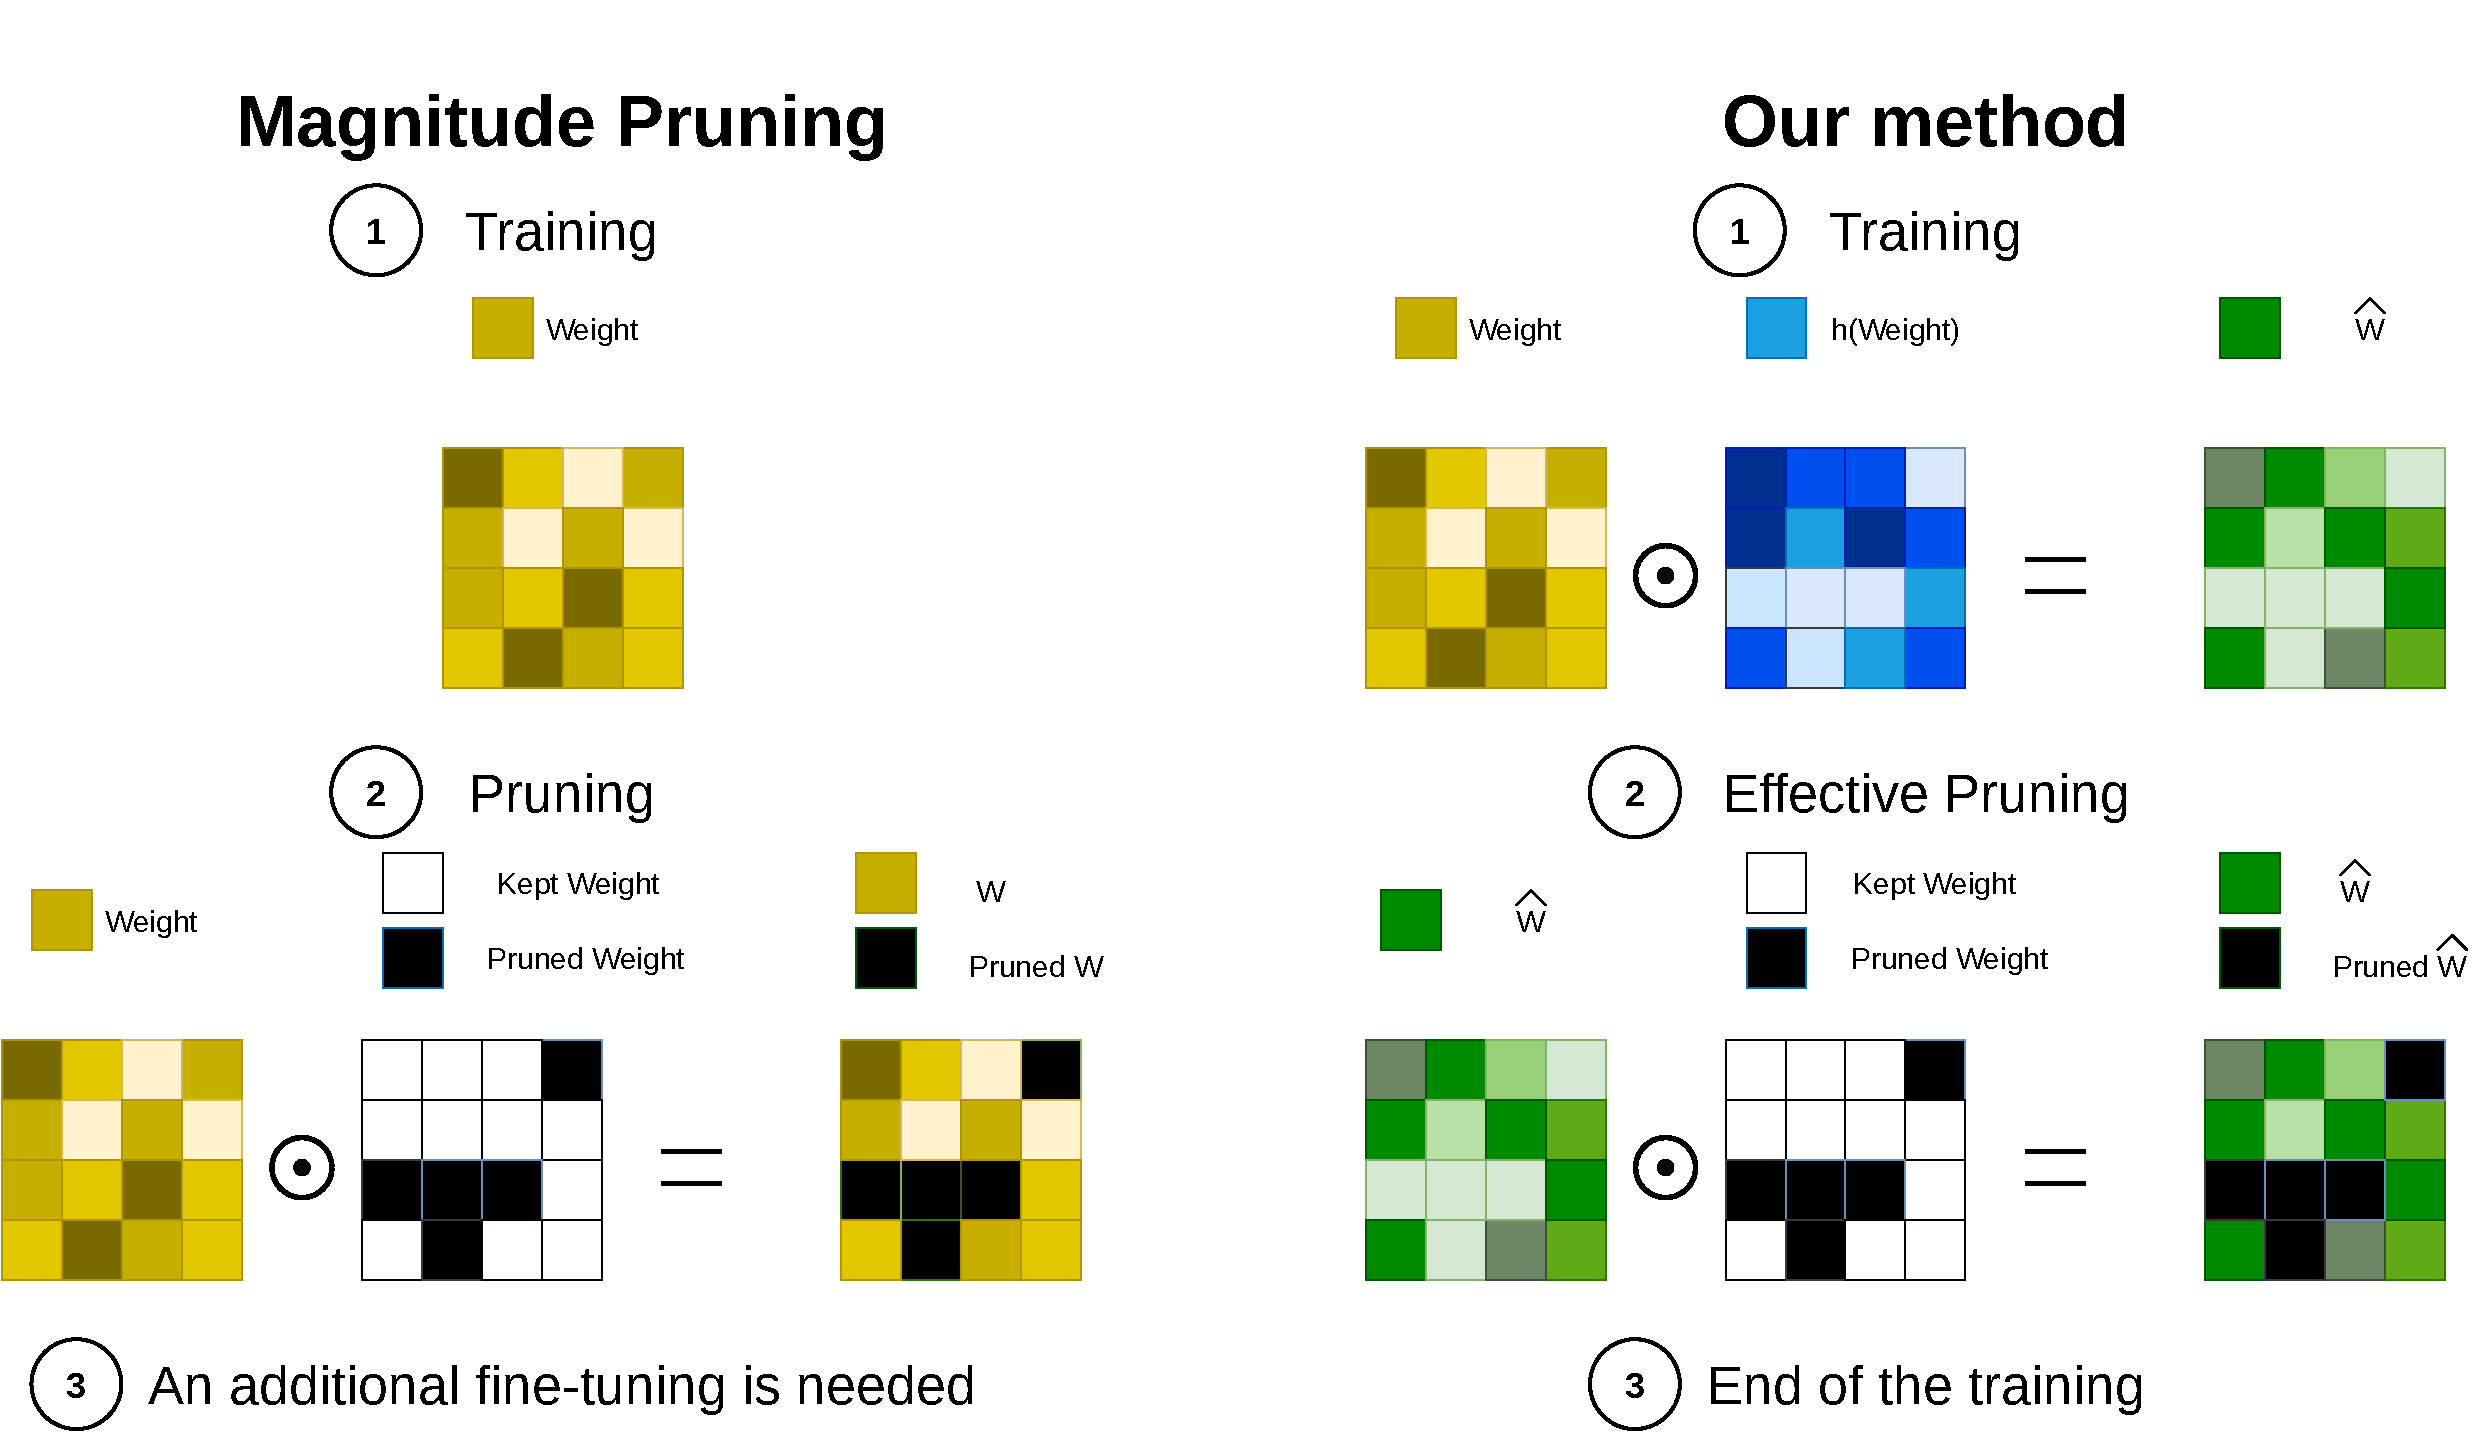
\includegraphics[width=12.5cm]{chapter_1/assets/comparison_reparam_vs_mag_pruning.pdf}}
  \caption{Comparison of our method and magnitude pruning. Magnitude pruning
  does not include any prior on weights during the initial training phase and
  needs an additional fine-tuning procedure. Our method embeds a saliency
  measure based on the weight magnitude in the reparametrisation and does not
  require fine-tuning. Best viewed in colour.}
  \label{fig:chap1:comparison_reparam_vs_mag_pruning}
\end{figure}


Our proposed framework allows for joint optimisation of the network weights and
topology. On the one hand, it prevents situations where, because of excessively
pruning a layer, the output from layer $\ell$ of the network is no longer
transmitted to layer $\ell+1$, a scenario we refer to as \emph{disconnections}.
These disconnections can lead to degenerate networks with an irrecoverable
performance drop. Due to these disconnections, the network output becomes
entirely uncorrelated with the input, and it becomes impossible to update the
weights located upstream of this disconnection. On the other hand, our framework
allows reaching a targeted pruning budget in a more convenient way than $\ell_1$
regularisation (see \cref{sec:chap1:impact_of_budget_loss}). Our
reparametrisation also helps minimising the performance drop between the
original and the pruned surrogate networks by maintaining competitive
performances without fine-tuning. Learning the weights values and the network
topology only requires one step that achieves pruning as a part of network
design. This step zeroes out the targeted number of connections by constraining
their reparametrised weights to vanish.

% endregion: introduction of method

\subsection{Weight Reparametrisation}
\label{sec:chap1:weight_reparam}
% region: weight reparam

We consider the original network $f$ as a stack of $L$ layers. The global
expression of $f$ can be recursively defined by the application of the layer
$\ell$ to the output of the layer $\ell-1$. Without a loss of generality, we
omit the bias for clarity. This expression is shown in
\cref{eqn:chap1:layer_eq_f}.
\begin{equation}
  \label{eqn:chap1:layer_eq_f}
  f(\mathbf{x}) = g_L \big(\mathbf{w}_L \cdot g_{L-1}(\mathbf{w}_{L-1} \cdot g_{L-2} \dots
  \mathbf{w}_2 \cdot g_1(\mathbf{w}_1 \cdot \mathbf{x}))\big),
\end{equation}
\noindent with $g_\ell$ being a nonlinear activation associated to $\ell \in
  \left\{ 1,\dots, L \right\}$ and $\left\{ \mathbf{w}_\ell \right\}_\ell$
denoting a set of weight tensors where each tensor is associated with a specific
layer $\ell$ in the network. Keeping the same topology but changing the values
of the weight, we now consider the surrogate network $\hat{f}$ with weights
$\{\mathbf{\hat{w}}_\ell\}_\ell$. \Cref{eqn:chap1:layer_eq_f} can be rewriten as
\cref{eqn:chap1:layer_eq_f_hat}. The activation function and the topology of $f$
and $\hat{f}$ are the same. Only the weights are updated.

\begin{equation}
  \label{eqn:chap1:layer_eq_f_hat}
  \hat{f}(\mathbf{x}) = g_L \big(\mathbf{\hat w}_L \cdot g_{L-1}(\mathbf{\hat w}_{L-1} \cdot g_{L-2}
  \dots\mathbf{\hat w}_2 \cdot g_1(\mathbf{\hat w}_1 \cdot \mathbf{x}))\big).
\end{equation}

\noindent In the above equation, $\mathbf{\hat w}_\ell$ is referred to as
\textit{apparent weight} tensor, which is a reparametrisation of
$\mathbf{w}_\ell$ that includes a prior on its saliency. An apparent weight
$\mathbf{\hat w}_\ell$ of $\hat{f}$ is derived from a \emph{latent weight}
$\mathbf{w}_\ell$ by applying the following reparametrisation:
\begin{equation}
  \label{eqn:chap1:reparam}
  \mathbf{\hat w}_\ell = \mathbf{w}_\ell  \odot h_t(\mathbf{w}_\ell),
\end{equation}
\noindent with $h_t$ being the reparametrisation function and $t$ its
temperature parameter (see \cref{eqn:chap1:h_star_expression}). Here, $\odot$
represents the Hadamard product. It means that it is element-wise, and every
single weight has its own reparametrisation. This reparametrisation function
enforces the prior that the smallest weights should be removed from the network
and acts as a surrogate $\ell_0$ norm for the budget loss (see
\cref{sec:chap1:budget_loss}). In order to achieve this objective, $h_t$ should
exhibit four properties: \\

\begin{enumerate}
  \item $\forall x \in \mathds{R},~~ 0 \leq h_t(x) \leq 1 $
  \item $h_t(x) \in C^1 \text{ on } \mathds{R}$
  \item $h_t(x) = h_t(-x)$
  \item $\forall a,\varepsilon \in\mathds{R}^{+\ast},~ \exists ~t
          \in\mathds{R}^{+\ast} ~ | ~ h_t(x) \leq \varepsilon, x \in [-a,a]$\\
\end{enumerate}

\noindent\textbf{First Property - Constrained Image} \\
\begin{equation}
  \centering
  \forall x \in \mathds{R},~~ 0 \leq h_t(x) \leq 1
  \label{eqn:chap1:reparam_prop1}
\end{equation}
\\
There should not be any co-adaptation between the weights and their
reparametrisation. In other words, the reparametrisation function should only
act as a means to select or not the weight. It should not act as a scaling
factor for the latent weight and scale it so that the apparent weight becomes
larger than the latent weight. Constraining the image prevents the value of the
weights from increasing rapidly to compensate for the removal of the smallest
weights. Finally, the apparent weights should have the same sign as the latent
weights. That is why the image of $\mathds{R}$ by $h_t$ should be the segment
$[0,1]$.\\

\noindent\textbf{Second Property - Differentiability} \\
\begin{equation}
  \centering
  h_t(x) \in C^1 \text{ on } \mathds{R}
  \label{eqn:chap1:reparam_prop2}
\end{equation}
\\
Our method should fit in the backpropagation framework \cite{rumelhart1986learning}. Since the optimisation will
be achieved by gradient descent, the reparametrisation function should be
differentiable to ensure a computable gradient.\\

\noindent\textbf{Third Property - Symmetry} \\

\begin{equation}
  \centering
  h_t(x) = h_t(-x)
  \label{eqn:chap1:reparam_prop3}
\end{equation}
\\
The reparametrisation function should not induce any bias toward the positive or
negative weights so that only their magnitudes matter. It implies that the
reparametrisation function should be symmetric.\\


\noindent\textbf{Fourth Property - Upper Bounded Segment} \\

\begin{equation}
  \centering
  \forall a,\varepsilon \in\mathds{R}^{+\ast},~ \exists ~t
  \in\mathds{R}^{+\ast} ~ | ~ h_t(x) \leq \varepsilon, x \in [-a,a]
  \label{eqn:chap1:reparam_prop4}
\end{equation}
\\
The last property ensures the existence of a temperature parameter $t$, which
allows upper-bounding the response of $h_t$ on any interval for any arbitrary
$\varepsilon$. More formally, for any arbitrarily large $a$ and arbitrarily
small $\varepsilon$, it exists a temperature $t$ which guarantees that $h_t(x)$
is smaller than $\varepsilon$, provided that $x$ is in the segment $[-a, a]$.
Hence, $h_t$ acts as a band-stop filter, eliminating the smallest weights where
the parameter $t$ controls the width of that filter.
\Cref{fig:chap1:reparam_funct_varying_t} shows the impact of $t$ on the shape of
the function, more precisely on the width of its pit, when the expression of
$h_t$ is set using \cref{eqn:chap1:stable_h_expression}.\\

\begin{figure}
  \centering
  \subfloat[$h_{t}$ with $t=1$ and varying $n$]{
    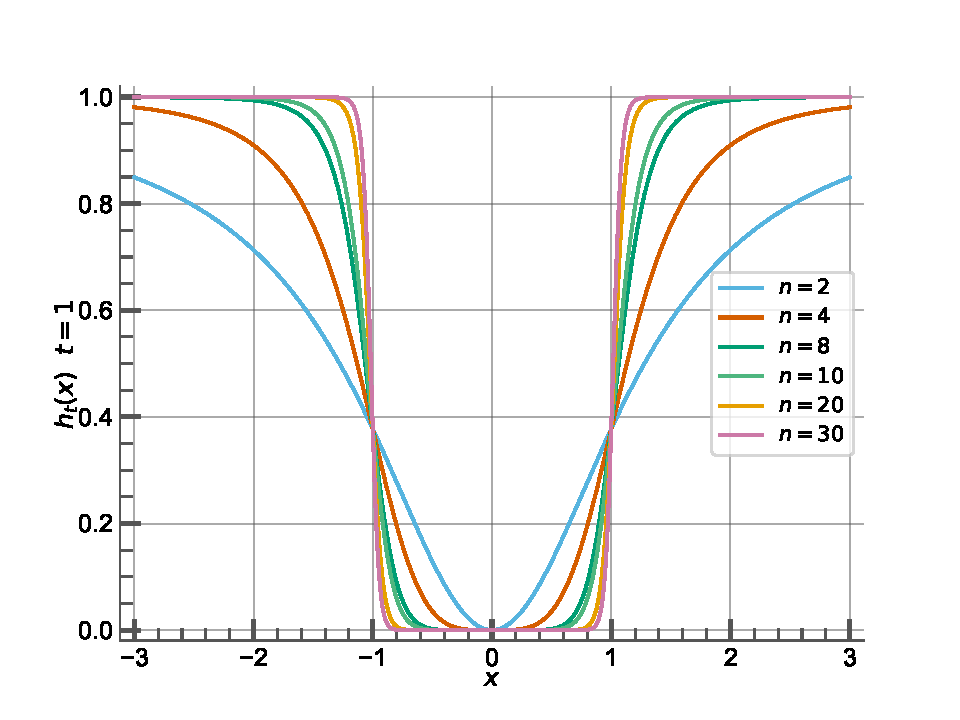
\includegraphics[width=0.49\linewidth]{chapter_1/assets/reparam_funct_varying_n.pdf}
    \label{fig:chap1:reparam_funct_varying_n}} \subfloat[$h_{t}$ with $n=2$
    and varying $t$]{
    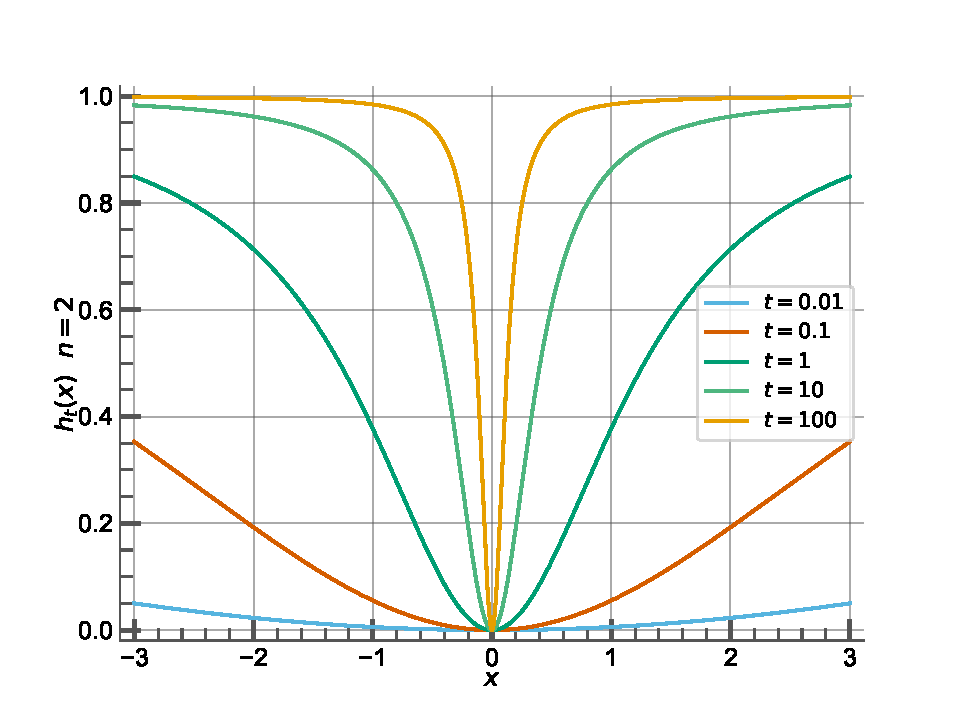
\includegraphics[width=0.49\linewidth]{chapter_1/assets/reparam_funct_varying_t.pdf}
    \label{fig:chap1:reparam_funct_varying_t}} \caption{
    Reparametrisation function $h_t$ with varying temperature parameter $t$ and
    power $n$. $t$ controls the width of the pit, and $n$ controls the steepness
    of the slope.}
  \label{fig:stopband}
\end{figure}

Weight distribution varies tremendously from one layer to another. In order to
match a specific budget (see \cref{sec:chap1:budget_loss}), the width of the
stopband, controlled by $t$, is tuned according to the weight distribution of
each layer. The manual setting of this parameter is non-trivial and cumbersome,
so in practice, $t$ is learned as a part of gradient descent on a layer-by-layer
basis.\\

Considering the aforementioned four properties of $h_t$, a simple choice of that
function is:
\begin{equation}
  \label{eqn:chap1:h_star_expression}
  \tilde{h}_t(x) = \exp\bigg\{{-\displaystyle\frac{1}{(tx)^n}}\bigg\}, ~ n\in 2\mathds{N},
\end{equation}
\noindent where $n$ controls the crispness of $\tilde{h}_t$. Here and in what
follows, $\tilde{h}_t$ denotes the expression of
\cref{eqn:chap1:h_star_expression} for the reparametrisation function. The
exponent $n$ is not considered as a parameter of $h_t$ (or $\tilde{h}_t$) since
we use a fixed value for our experiments (\cref{sec:chap1:experiments}), whereas
$t$ is a learnt parameter and varies from one layer to another.
\Cref{fig:chap1:reparam_funct_varying_n} shows the impact of n on the general
sharpness of the function. Although the function whose expression is given in
\cref{eqn:chap1:h_star_expression} satisfies the four above properties, in
practice, $\tilde{h}_t$ suffers from numerical instability as it generates
\ac{nan} outputs in most of the widely used deep learning frameworks. Due to the
way backpropagation works, a single \ac{nan} in a weight tensor makes the whole
optimisation process for the entire network no longer possible. We consider
instead a stabilised variant with similar behaviour, as
\cref{eqn:chap1:h_star_expression},  that still satisfies the four above
properties. This numerically stable variant is defined as:
\begin{equation}
  \label{eqn:chap1:stable_h_expression}
  h_t(x) = C_1 \biggl( \text{exp} \bigg\{-\displaystyle\frac{1}{(tx)^n +1}\bigg\} - C_2 \biggr),
\end{equation}
\noindent with $C_1=\frac{1}{1-e^{-1}}$ and $C_2 = e^{-1}$. In what follows, we
use the expression of \cref{eqn:chap1:stable_h_expression} for the
reparametrisation function $h_t$, whereas $\tilde{h}_t$ refers to the expression
of \cref{eqn:chap1:h_star_expression}, which is its numerically unstable
version.\\

The addition of the scalar value 1 at the denominator in
\cref{eqn:chap1:stable_h_expression} is a way to achieve numerical stability. In
\cref{eqn:chap1:h_star_expression}, the denominator $(tx)^n$ has the potential
to approach very small values that result in numerical instabilities, leading to
\ac{nan} outputs. The addition of 1 to the denominator makes the function
numerically stable and avoids producing \ac{nan} outputs. This solution is
favoured over adding a small value, such as an arbitrarily small $\varepsilon$,
as the latter requires careful consideration of its magnitude and may result in
either dramatic alterations to the shape of the function or continued numerical
instability if not carefully chosen. The addition of the value 1 to the
denominator provides a straightforward and sufficient mean to stabilise the
function. Constants $C_1$ and $C_2$ are introduced to compensate for the slight
alterations to the shape of the function caused by the addition of 1 to the
denominator, and thus, to ensure that the first property
(\cref{eqn:chap1:reparam_prop1}) is satisfied. Although both $\tilde{h}_t$ and $h_t$
satisfy the four properties, they do not have the exact same shapes, as
illustrated in figure (\ref{fig:chap1:h_stable_vs_unstable}).\\

In the next sections, the application of function $h_t$ to a multi-dimensional
tensor is element-wise. Consequently $h_t(\mathbf{z})$ denotes the tensor whose
entries are the result of applying $h_t$ to each one of the corresponding
entries of $\mathbf{z}$.\\

\begin{figure}
  \centering
  \centerline{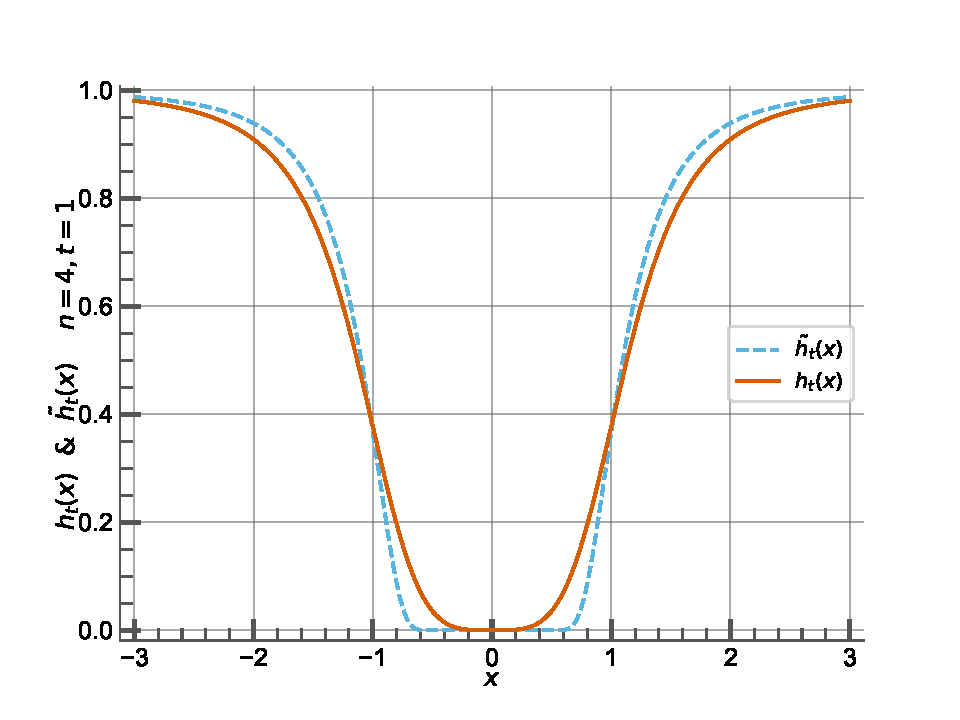
\includegraphics[width=0.49\linewidth]{chapter_1/assets/h_stable_vs_unstable.pdf}}
  \caption{ The unstable reparametrisation function $\tilde{h}_t$ and its
    stable alternative $h_t$, with $t=1$ and $n=4$ for both functions.}
  \label{fig:chap1:h_stable_vs_unstable}
\end{figure}
% endregion: weight reparam

\subsection{Budget Loss}
\label{sec:chap1:budget_loss}
% region: budget loss
Most of the traditional pruning methods in deep learning do not explicitly
incorporate the targeted weight budget during optimisation. The amount of
weights pruned is typically enforced post-training, which may lead to suboptimal
results compared to methods that consider the weight budget during optimisation.
Our method introduces a budget loss, in addition to the main task loss, that
drives the network to match and satisfy a given weight budget during the
training process. Consequently, the trained network can be pruned to the desired
pruning rate with a marginal loss in performance without fine-tuning.\\


The considered budget is weight-based and should quantify the targeted fraction
of active connections in the network. To build the budget loss, we first
introduce a cost function that quantifies the number of active connections in
the network. Let $C(\{\mathbf{w}_1,\dots, \mathbf{w}_L\})$ be the {\em observed}
cost associated to a neural network and $C_\text{target}$ the {\em targeted}
one. $C_\text{target}$ is the number of connections that should be active at the
end of the training procedure. The budget loss is defined as \\

\begin{equation}
  \label{eqn:chap1:simple_budget}
  {\cal L}_\text{budget} = \bigl( C(\{\mathbf{w}_1,\dots, \mathbf{w}_L\}) - C_\text{target} \bigr)^2.
\end{equation} \\


\noindent This budget loss is combined with the main task loss (a classification
loss in our experiments - see \cref{sec:chap1:experiments}). The budget loss $
  {\cal L}_\text{budget}$ is quadratic in order to ensure the minimisation of the
difference between the {\em observed} and the {\em targeted} costs. For better
conditioning of this combination, we normalise the budget loss by
$C_\text{initial}$. The latter corresponds to the cost of the original unpruned
network, which is set in practice to the number of its parameters (see also
\cref{sec:chap1:experiments}). Hence, \cref{eqn:chap1:simple_budget} is updated
as:\\

\begin{equation}
  \label{eqn:chap1:real_budget}
  {\cal L}_\text{budget} = \biggl( \displaystyle\frac{C(\{\mathbf{w}_1,\dots, \mathbf{w}_L\}) - C_\text{target}}{C_\text{initial}} \biggr)^2.
\end{equation}\\

Finally, the two losses are combined together via a strictly positive mixing
hyperparameter $\lambda$ that controls the relative importance of the budget loss
${\cal L}_\text{budget}$ compared to the main task loss ${\cal L}_\text{task}$,
leading to\\

\begin{equation}
  \label{eqn:chap1:globalloss}
  {\cal L} =  {\cal L}_\text{task} + \lambda \cdot {\cal L}_\text{budget}.
\end{equation} \\

Ideally, the budget of a neural network could be evaluated as the number of
multiply-add operations, often referred to as \acp{FLOP} or
\acp{MAC}\footnote{The number of \ac{MAC} operations  or \acp{FLOP} for a layer
  cannot be fully determined by its number of parameters since it is heavily
  dependent on the input size. More details are given in
  \cref{sec:appendix:macs}}, needed for a forward pass or through the $\ell_0$
norm of its weights. However, neither are known to be differentiable and,
therefore, cannot be used in a gradient-based optimisation. In order to
circumvent these limitations, we use our weight reparametrisation as a surrogate
measure of $\ell_0$, and we define the cost function as in
\cref{eqn:chap1:cost_function}.\\

\begin{equation}
  \label{eqn:chap1:cost_function}
  C(\{\mathbf{w}_1,\dots, \mathbf{w}_L\}) = \displaystyle \sum_{\ell=1}^{L} \sum_{i=1}^{\nu_\ell} h_t(\mathbf{w}_{\ell i}).
\end{equation} \\


\begin{figure}
  \centering
  \subfloat[Number of parameters]{
    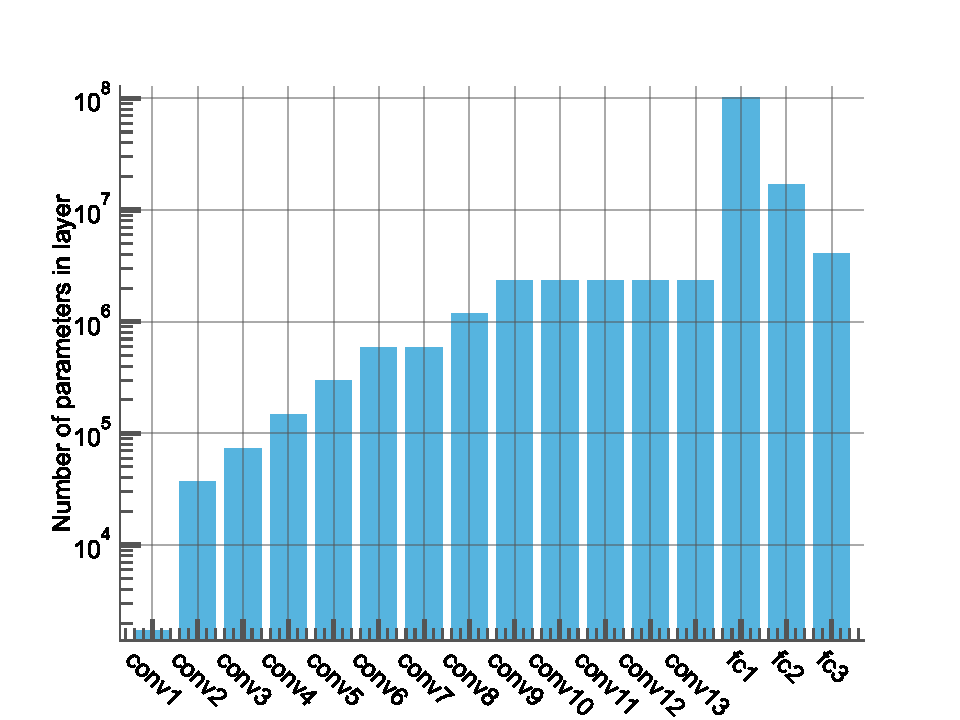
\includegraphics[width=0.49\linewidth]{chapter_1/assets/vgg16_num_params_per_layer.pdf}
    \label{fig:chap1:num_parap_vgg16}} \subfloat[Normalisation factor]{
    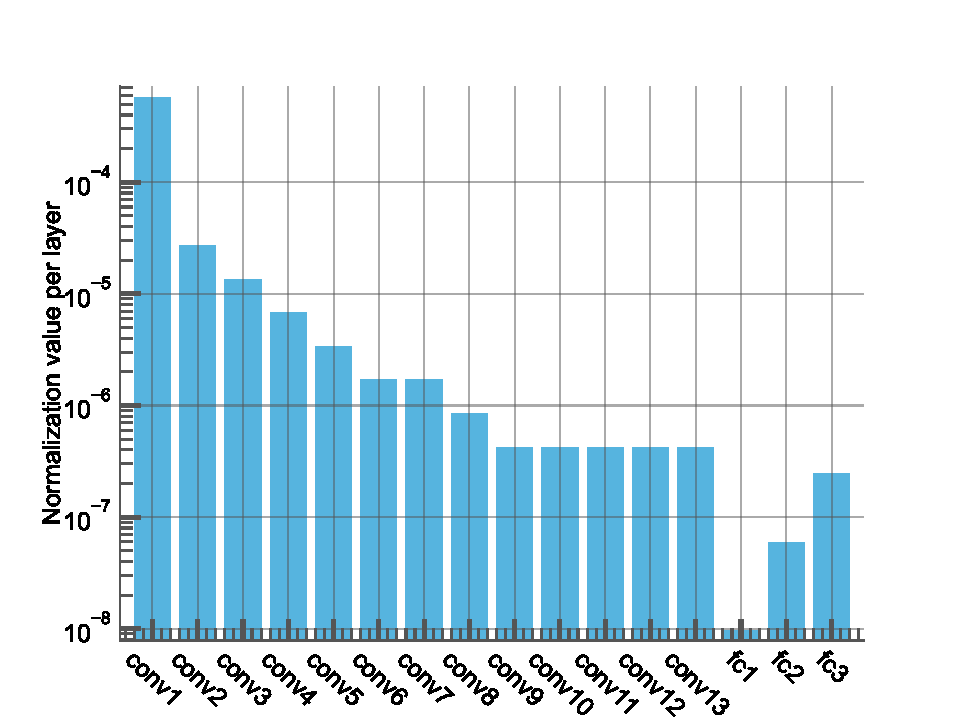
\includegraphics[width=0.49\linewidth]{chapter_1/assets/vgg16_normalization_factor_per_layer.pdf}
    \label{fig:chap1:norm_factor_vgg16}} \caption{ Log-scale plot of
    number of parameters and normalisation factor per layer for a VGG16
    network. The significant differences in terms of the number of parameters
    yields dramatically different normalisation factors. Some of them are 4
    orders of magnitude apart, and all of them are vanishingly small compared
    to a common main task loss value.}
  \label{fig:chap1:vgg16_per_layer_param_and_norm_factor}
\end{figure}

One may argue that the cost should be normalised layer-wise and, therefore,
that the right-hand term of \cref{eqn:chap1:cost_function} should be written as

$$\displaystyle\sum_{\ell=1}^{L}\frac{\displaystyle \sum_{i=1}^{\nu_\ell}
    h_t(\mathbf{w}_{\ell i})}{\nu_\ell}$$

However, the number of elements in a layer greatly varies from one to another
(as displayed in \cref{fig:chap1:vgg16_per_layer_param_and_norm_factor}). As a
result,  the budget loss relative importance would vary from one layer to
another. More importantly, the optimisation process would have less incentive to
introduce sparsity in larger layers since their normalisation factor would make
the budget loss negligible compared to other layers or the main task loss. This
is critical since the large layers are generally the ones where the highest
pruning rates can be achieved \cite{DBLP:journals/corr/abs-2202-12002}.
Regarding the aforementioned reasons, a better alternative is to normalise by
the initial cost $C_\text{initial}$, as done in \cref{eqn:chap1:real_budget}.\\

% endregion : budget loss

\section{Method and Algorithm Overview}
\label{sec:chap1:overview}
% region : overview 
Our method is a combination of a weight reparametrisation and a budget loss,
both described in the previous sections. The two are combined in a global method
that can be used in a standard training procedure using gradient descent. Once
the neural network trained using the method detailed in
\cref{sec:chap1:pruning}, we proceed to prune the smallest weights, w.r.t. their
magnitude, to match and enforce the predetermined targeted budget. During this
stage, we set the smallest weights to zero until the budget requirement is met.
This process is referred to as \textit{effective pruning}.\\

In
\cref{sec:chap1:performances,sec:chap1:impact_of_lambda,sec:chap1:impact_of_reparametrisation,sec:chap1:impact_of_budget_loss}
our results are obtained after following this procedure, which is described in
\cref{alg:chap1:training_pruning}. In other words, the network is first trained
with our reparametrisation and our budget loss, then the \textit{effective
  pruning} step is applied, and finally, the performance is evaluated. In
\cref{sec:chap1:impact_of_fine_tuning}, we assess the performance of our method
with an already trained and pruned initalisation. In this precise setup, since
the initialisation is already pruned to match the targeted budget, the
\emph{effective pruning} step is not needed and thus not applied.\\

\begin{algorithm}
  \caption{Our training procedure}
  \label{alg:chap1:training_pruning}
  \begin{algorithmic}
    \REQUIRE Dataset $\mathcal{D} \subset \mathcal{X} \times \mathcal{Y}$, network $f$,
    weights $\theta$, number of epochs $E$, mixing coefficient $\lambda$, learning
    rate $\eta$, pruning rate $p$
    \FOR{$t = 1$ to $E$}
    \FOR{each $(X,y) \in \mathcal{D}$}
    % \STATE $f(X; \theta_t)$ \COMMENT{Compute the output of the network}
    \STATE $\mathcal{L}= \mathcal{L}_{task}(y, f(X, \theta_t)) + \lambda \cdot
      \mathcal{L}^{p}_{budget}(\theta_t )$ \COMMENT{Compute the loss: task loss
      and budget loss}
    \STATE $\theta_{t+1} = \theta_t - \eta \nabla_{\theta} \mathcal{L}$ \COMMENT{Backpropagate the loss and update the weights}
    \ENDFOR
    \ENDFOR
    \RETURN Trained network $f$
    \STATE Perform \emph{effective pruning} on the weights $\theta$: set to 0 the
    smallest $p$\% of the weights $w\in\theta$
    \RETURN Trained and pruned network $f$
  \end{algorithmic}
\end{algorithm}


The reader can grasp a better understanding of the key differences of our method
compared to the standard pruning pipeline that applies to most pruning methods,
not only magnitude pruning method, by looking at
\cref{fig:chap1:pruning_pipeline_comparison}. It highlights the fact that the
targeted pruning rate is taken into account from the beginning thanks to the
budget loss, and therefore, the network does not need a fine-tuning step after
the \emph{effective pruning} step. On the contrary, the standard pruning
pipeline applies the \emph{pruning criterion} and the \emph{effective pruning}
after the initial training. This results in a drop in performance that needs to
be compensated for with fine-tuning. \\

\begin{figure}
  \centering
  \subfloat[Our Pipeline\label{fig:chjap1:our_pipeline}]{
    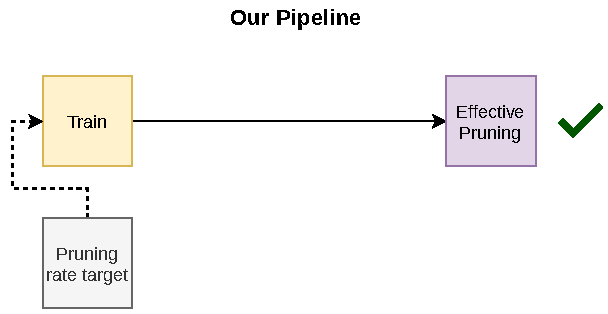
\includegraphics[width=0.49\textwidth]{chapter_1/assets/pipeline_comparison_with_pruning_reparam_pr.pdf}}
    \subfloat[Standard Pruning
    Pipeline\label{fig:chap1:standard_pruning_pipeline}]{
    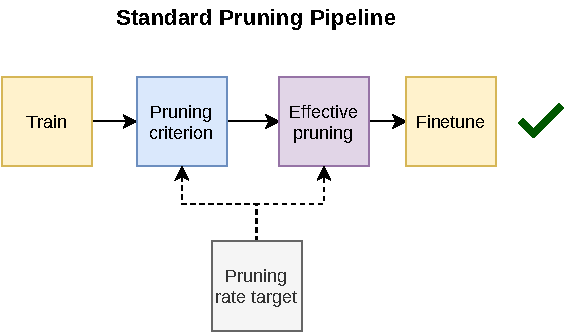
\includegraphics[width=0.49\textwidth]{chapter_1/assets/pipeline_comparison_with_pruning_mag_pr.pdf}}
    \caption{ Principle scheme of our pruning pipeline and the standard pruning
    pipeline. With our pruning pipeline, the targeted pruning rate that will be
    enforced during the \emph{effective pruning} step, is taken into account
    from the beginning. Thus, our method does not need a fine-tuning step. In
    contrary, the standard pruning pipeline applies the \DIFdelbeginFL \emph{\DIFdelFL{pruing criterion}}
    %DIFAUXCMD
\DIFdelendFL \DIFaddbeginFL \emph{\DIFaddFL{pruning criterion}}
    \DIFaddendFL and the \emph{effective pruning} after the initial training. This results in
    a drop in performance that needs to be compensated for with fine-tuning.}
  \label{fig:chap1:pruning_pipeline_comparison}
\end{figure}

% endregion: overview

\section{Experiments}\label{sec:chap1:experiments}

% region : experiments
% region: introduction of the experiments
In this section, we will study the effectiveness of our method for compressing
\aclp{CNN} image classification models, as well as its impact on accuracy. To
that extent, we will review the impact of both our reparametrisation and our
budget loss. \DIFdelbegin \DIFdel{To that extent}\DIFdelend \DIFaddbegin \DIFadd{For this purpose}\DIFaddend , we use three reference databases in the field of
computer vision: CIFAR-10 \cite{CIFARdataset}, CIFAR-100 \cite{CIFARdataset},
and TinyImageNet \cite{TinyImageNet}, \DIFdelbegin \DIFdel{presentend }\DIFdelend \DIFaddbegin \DIFadd{presented }\DIFaddend in \cref{sec:dlo:datasets}. We
will evaluate the impact of our method on several neural network architectures:
VGG16 \cite{DBLP:journals/corr/SimonyanZ14a}, Conv4
\cite{DBLP:conf/iclr/FrankleC19}, ResNet18, and ResNet20
\cite{DBLP:conf/cvpr/HeZRS16}, introduced in
\cref{sec:dlo:architectures_used}.\\

% endregion: introduction of the experiments

\subsection{Experimental Setup}\label{sec:chap1:experimental_setup}

Performances of our method are evaluated on CIFAR-10 and CIFAR-100 with Conv4,
VGG16 and ResNet20. On TinyImageNet, we evaluate our method on ResNet18. We
compare our method against magnitude pruning \cite{DBLP:conf/nips/HanPTD15}. The
key differences between our method and magnitude pruning are the following:
$(i)$ our method uses a budget loss to encourage sparsity, which takes into
account the final pruning rate from the beginning of the training process and
$(ii)$ our method does not require fine-tuning after pruning. Because of the
latter, we compare our method against magnitude pruning with and without
fine-tuning. Both methods share the following setup: networks are trained during
300 epochs with an initial learning rate of $0.1$. A \emph{Reduce On Plateau}
policy is applied to the learning rate: if the validation accuracy is not
improving for 10 epochs in a row, then the learning rate is decreased by a
factor of $0.3$. A weight decay is applied on the weights with a penalisation
factor of $5\times10^{−5}$. This value is lower than the more conventional value
of $1\times10^{-4}$, because we want some weights to be able to drift away from
the origin, and therefore, escape from the pit of $h_t$. An Early Stopping
policy was used to stop the training prematurely if no improvement in the test
accuracy is observed in 60 epochs. To keep the comparison fair, for magnitude
pruning, the 300 epochs are split into two phases: the first 150 epochs are
dedicated to the training of the network, and the last 150 epochs are used for
fine-tuning the pruned network. In the fine-tuning phase, the learning rate is
divided by 100 for better convergence. \\


\subsection{Performances}\label{sec:chap1:performances}
% region: performances

Results are reported on
\cref{fig:chap1:reparam_vs_mpft_conv4,fig:chap1:reparam_vs_mpft_resnet20,fig:chap1:reparam_vs_mpft_vgg16}.
In these figures, our method (denoted \emph{Ours}) is compared to magnitude
pruning with and without fine-tuning (denoted \emph{MP w/ FT} and \emph{MP w/o
  FT}, respectively). All three methods are evaluated on the test set of the
dataset once the network has been pruned up to the pruning rate indicated on the
\emph{x-axis}. The test accuracy is reported on the \emph{y-axis} as a float
between 0 and 1 (0 being all images wrongly classified and 1 being all images
correctly classified). Each solid line representing a method is the mean of 5
independent runs. The coloured area surrounding the solid line represents the
standard deviation. In addition to the three methods, the dashed lines represent
the performances of an unpruned network trained without weight reparametrisation
and budget loss (denoted \emph{baseline}) and the accuracy of our method before
the effective pruning (denoted \emph{Ours (pre pruning)}), i.e. before we set
the smallest weight, w.r.t. their magnitude, to zero. Sub-figures (c) and (d) of
\cref{fig:chap1:reparam_vs_mpft_conv4,fig:chap1:reparam_vs_mpft_resnet20,fig:chap1:reparam_vs_mpft_vgg16}.
represents the number of epochs (\emph{y-axis}) needed to obtain the best model
for each method, depending on the pruning rate (\emph{x-axis}).\\


Overall, our method performs consistently better than magnitude pruning without
fine-tuning (\emph{MP w/o FT}) and, for almost all pruning rates, better than
magnitude pruning with fine-tuning (\emph{MP w/ FT}) on the CIFAR-10 and
CIFAR-100 datasets. In particular, our method significantly outperforms
magnitude pruning in both setups (with and without fine-tuning) for Conv4
networks (cf. \cref{fig:chap1:reparam_vs_mpft_conv4_cifar10}). For the VGG16
network, we observe the same trend, although the difference is less significant.
For ResNet20, magnitude pruning slightly overtakes our method on CIFAR-100 for
high pruning rates (more than 90\%).
\Cref{fig:chap1:reparam_vs_mpft_conv4_cifar10_epochs,fig:chap1:reparam_vs_mpft_conv4_cifar100_epochs,fig:chap1:reparam_vs_mpft_vgg16_cifar10_epochs,fig:chap1:reparam_vs_mpft_vgg16_cifar100_epochs,fig:chap1:reparam_vs_mpft_resnet20_cifar10_epochs,fig:chap1:reparam_vs_mpft_resnet20_cifar100_epochs}
show that our method requires an equivalent number of epochs compared to
magnitude pruning for a higher level of performance (\textit{i.e.} a higher test
accuracy). Magnitude pruning requires fewer epochs than our method, only at high
pruning rates (more than 90\%). On TinyImageNet
(\cref{fig:chap1:reparam_vs_mpft_resnet18}), our method outperforms magnitude
pruning with and without fine-tuning including at very high pruning rates
(95\%). In all scenarios
(\cref{fig:chap1:reparam_vs_mpft_conv4,fig:chap1:reparam_vs_mpft_vgg16,fig:chap1:reparam_vs_mpft_resnet20,fig:chap1:reparam_vs_mpft_resnet18}),
our method produces much more stable results, and variations from one run to
another are significantly smaller than the ones in magnitude pruning. Indeed,
the combination of the reparametrisation and the budget loss \DIFdelbegin \DIFdel{act}\DIFdelend \DIFaddbegin \DIFadd{acts}\DIFaddend , on the one
hand, as a regulariser and, on the other hand, helps to prepare the network for
the effective pruning step.\\

% region: perfs_figures
\begin{figure}
  \centering
  \subfloat[Conv4 - CIFAR-10]{
    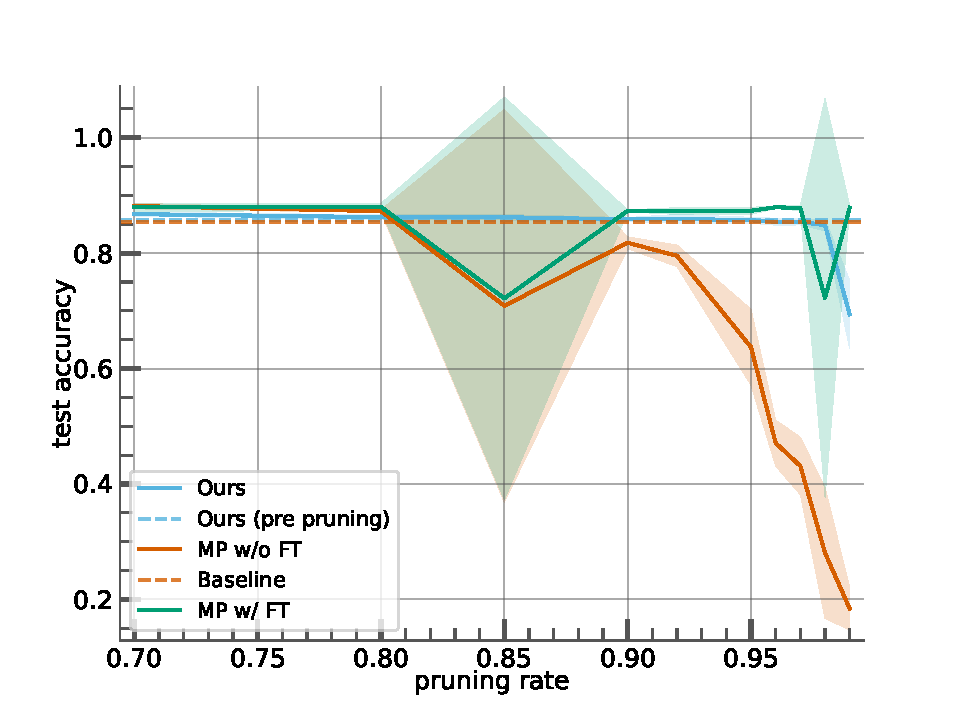
\includegraphics[width=0.49\linewidth]{chapter_1/assets/reparam_vs_mpft_Conv4_cifar10.pdf}
    \label{fig:chap1:reparam_vs_mpft_conv4_cifar10}}
  \subfloat[Conv4 - CIFAR-100]{
    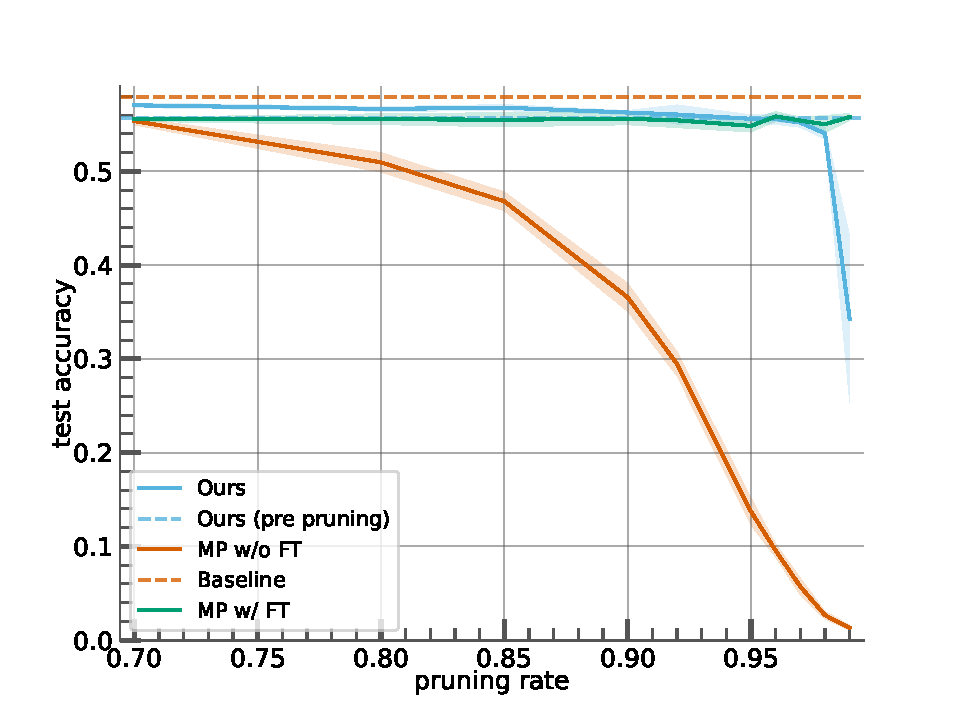
\includegraphics[width=0.49\linewidth]{chapter_1/assets/reparam_vs_mpft_Conv4_cifar100.pdf}
    \label{fig:chap1:reparam_vs_mpft_conv4_cifar100}}
  \\
  \subfloat[Conv4 - CIFAR-10 (Number of Epochs)\label{fig:chap1:reparam_vs_mpft_conv4_cifar10_epochs}]{
    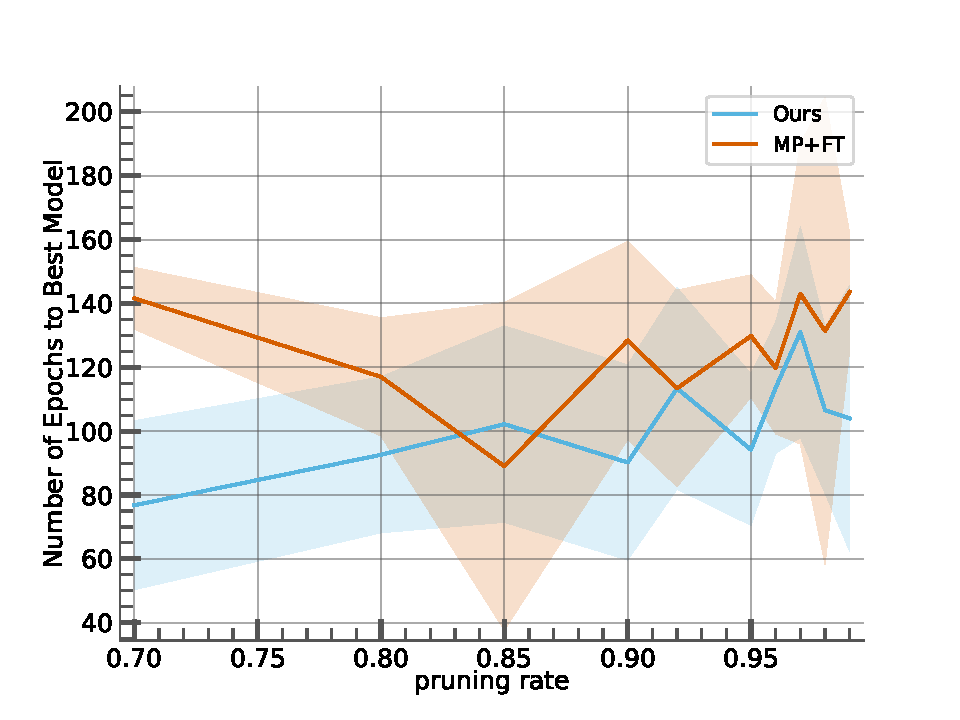
\includegraphics[width=0.49\linewidth]{chapter_1/assets/reparam_vs_mpft_training_time_Conv4_cifar10.pdf}}
  \subfloat[Conv4 - CIFAR-100 (Number of Epochs)\label{fig:chap1:reparam_vs_mpft_conv4_cifar100_epochs}]{
    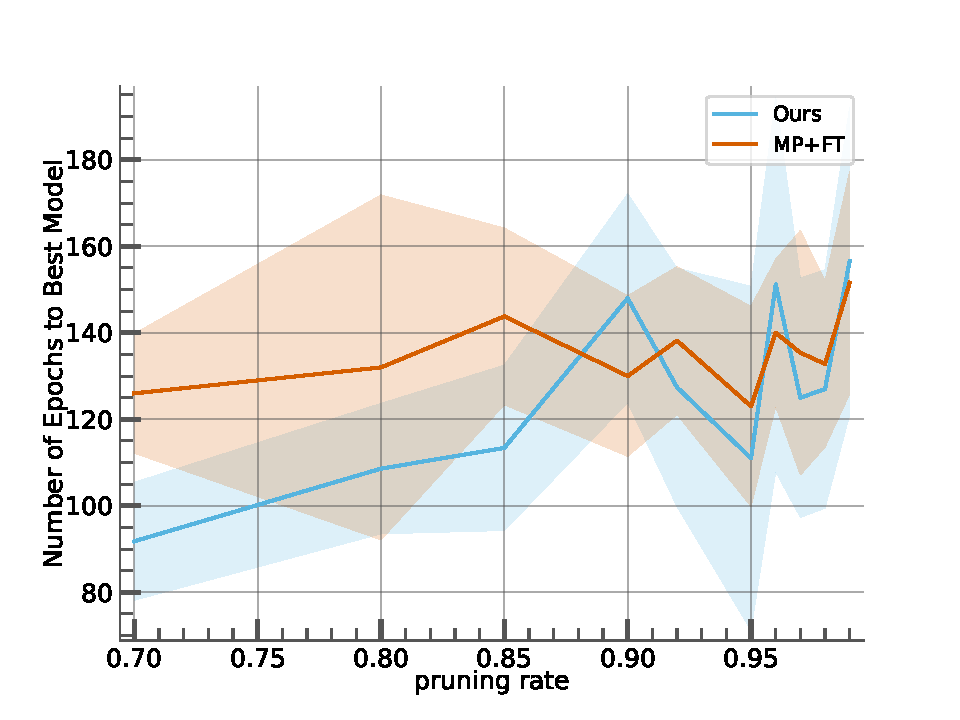
\includegraphics[width=0.49\linewidth]{chapter_1/assets/reparam_vs_mpft_training_time_Conv4_cifar100.pdf}}
  \caption{ Performances comparison of our method {\em(Ours)} against
  magnitude pruning without {\em(MP w/o FT)} and with fine-tuning {\em(MP w/ FT)} with a Conv4 network on
  CIFAR-10 and CIFAR-100 datasets, for different pruning rates.
  \Cref{fig:chap1:reparam_vs_mpft_conv4_cifar10} and
  \cref{fig:chap1:reparam_vs_mpft_conv4_cifar100} show the testing accuracy of
  the model and \cref{fig:chap1:reparam_vs_mpft_conv4_cifar10_epochs} and
  \cref{fig:chap1:reparam_vs_mpft_conv4_cifar100_epochs} the number of epochs
  needed to obtain the best model. Best viewed in colours.}
  \label{fig:chap1:reparam_vs_mpft_conv4}
\end{figure}

\begin{figure}
  \centering
  \subfloat[VGG16 - CIFAR-10]{
    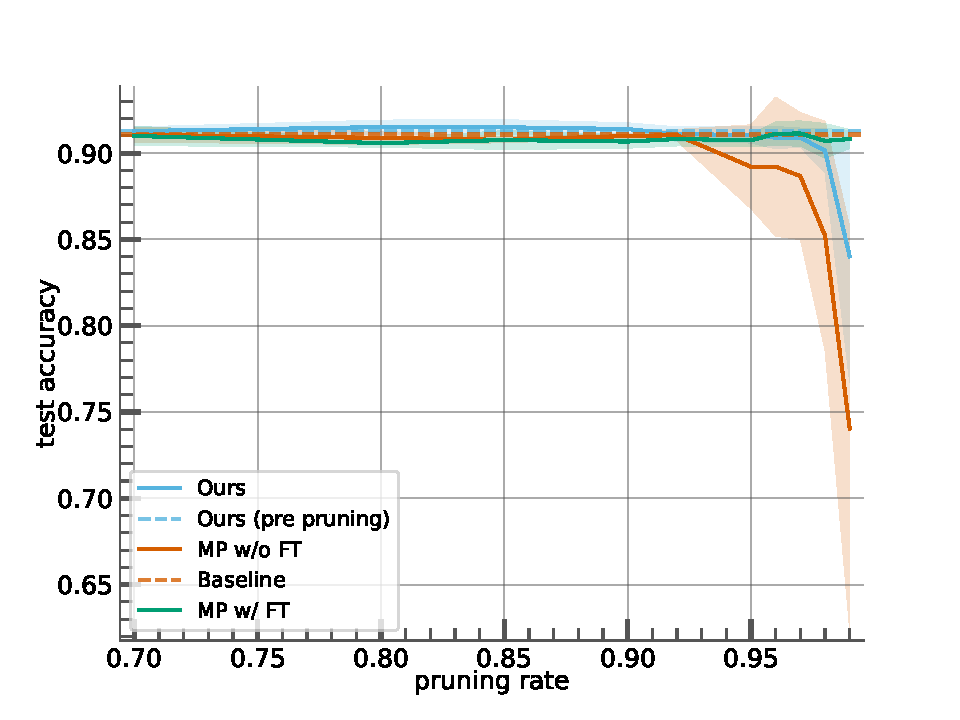
\includegraphics[width=0.49\linewidth]{chapter_1/assets/reparam_vs_mpft_PrunableVGG16_cifar10.pdf}
    \label{fig:chap1:reparam_vs_mpft_vgg16_cifar10}}
  \subfloat[VGG16 - CIFAR-100]{
    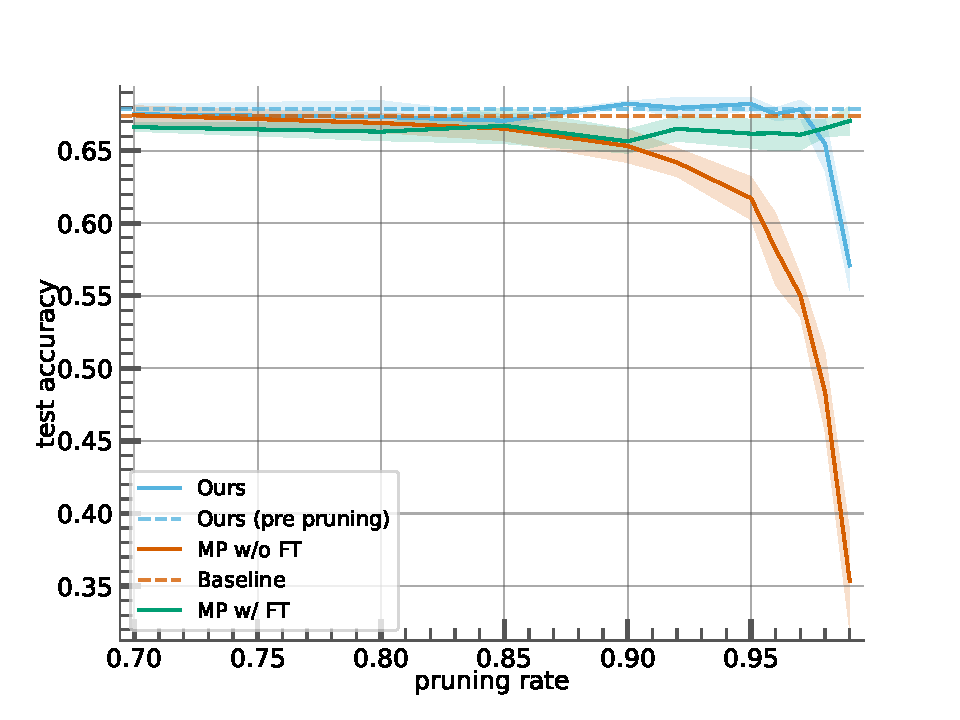
\includegraphics[width=0.49\linewidth]{chapter_1/assets/reparam_vs_mpft_PrunableVGG16_cifar100.pdf}
    \label{fig:chap1:reparam_vs_mpft_vgg16_cifar100}}
  \\
  \subfloat[VGG16 - CIFAR-10 (Number of Epochs)\label{fig:chap1:reparam_vs_mpft_vgg16_cifar10_epochs}]{
    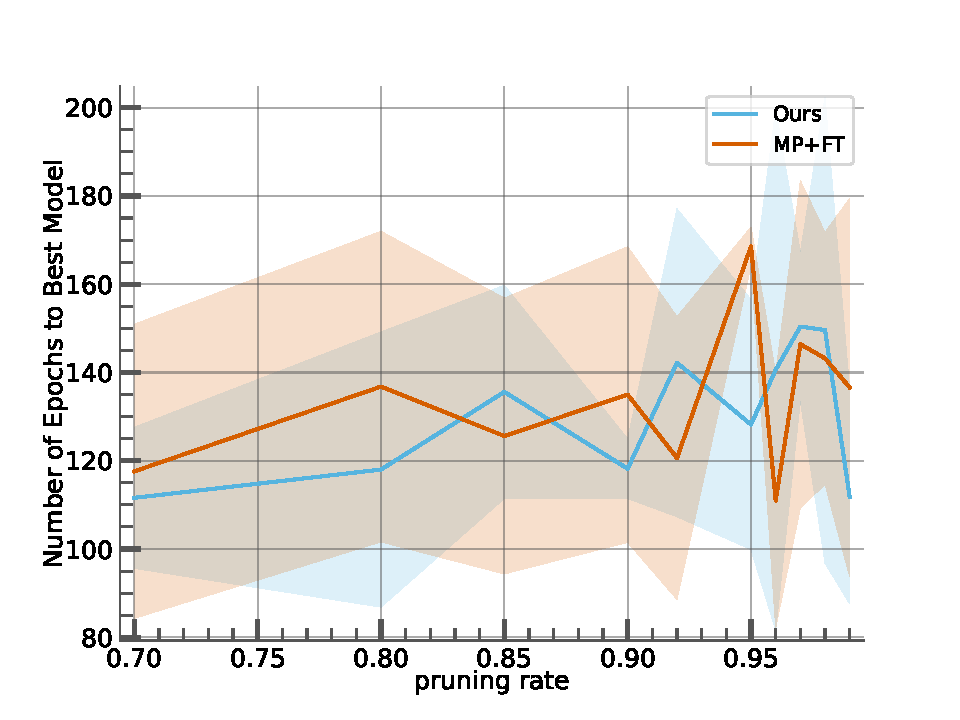
\includegraphics[width=0.49\linewidth]{chapter_1/assets/reparam_vs_mpft_training_time_PrunableVGG16_cifar10.pdf}}
  \subfloat[VGG16 - CIFAR-100 (Number of Epochs)\label{fig:chap1:reparam_vs_mpft_vgg16_cifar100_epochs}]{
    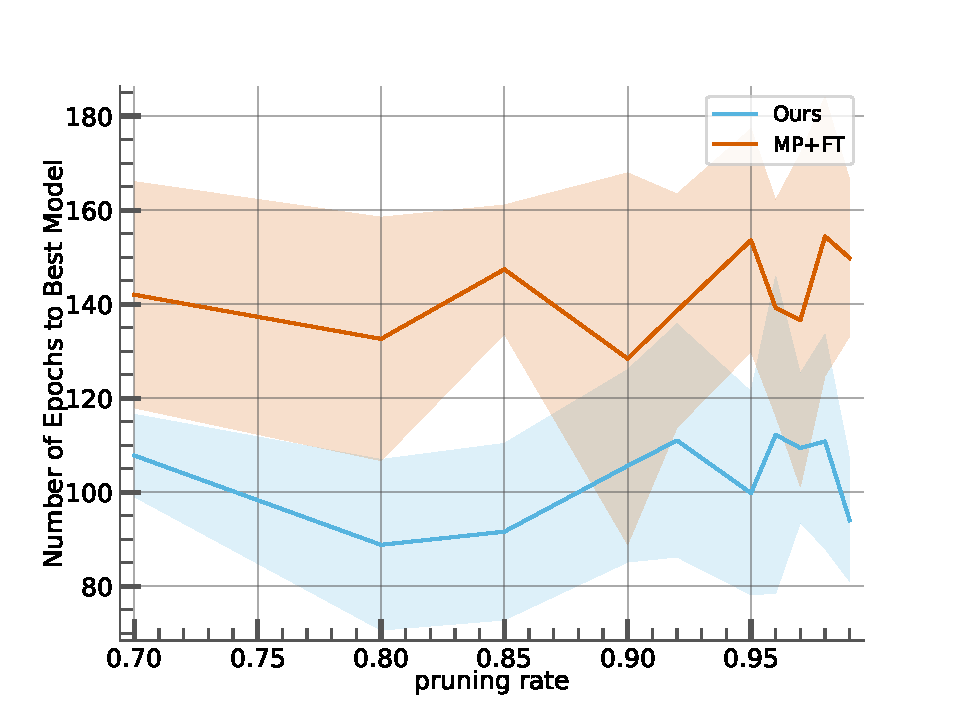
\includegraphics[width=0.49\linewidth]{chapter_1/assets/reparam_vs_mpft_training_time_PrunableVGG16_cifar100.pdf}}


  \caption{ Performances comparison of our method \em{(Ours)} against
    magnitude pruning with fine-tuning \em{(MP+FT)} with a VGG16 network on
    CIFAR-10 and CIFAR-100 datasets, for different pruning rates.
    \Cref{fig:chap1:reparam_vs_mpft_vgg16_cifar10} and
    \cref{fig:chap1:reparam_vs_mpft_vgg16_cifar100} show the testing accuracy of
    the model and \cref{fig:chap1:reparam_vs_mpft_vgg16_cifar10_epochs} and
    \cref{fig:chap1:reparam_vs_mpft_vgg16_cifar100_epochs} the
    number of epochs needed to obtain the best model. Best viewed in colours.}
  \label{fig:chap1:reparam_vs_mpft_vgg16}
\end{figure}

\begin{figure}
  \centering
  \subfloat[ResNet20 - CIFAR-10\label{fig:chap1:reparam_vs_mpft_resnet20_cifar10}]{
    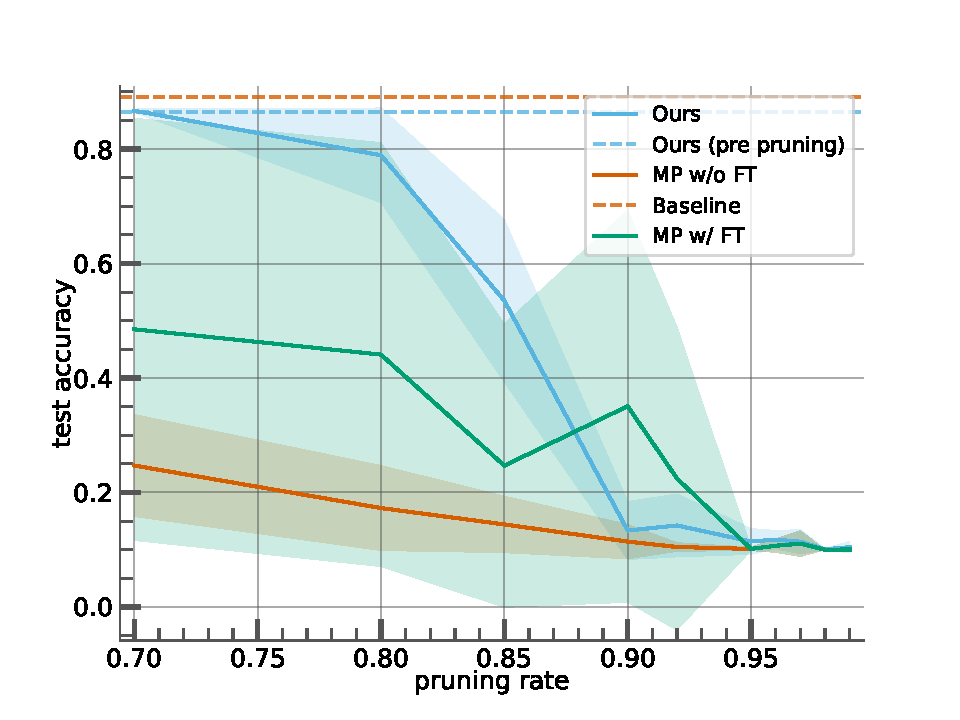
\includegraphics[width=0.49\linewidth]{chapter_1/assets/reparam_vs_mpft_PrunableResNet20_cifar10.pdf}}
  \subfloat[ResNet20 - CIFAR-100\label{fig:chap1:reparam_vs_mpft_resnet20_cifar100}]{
    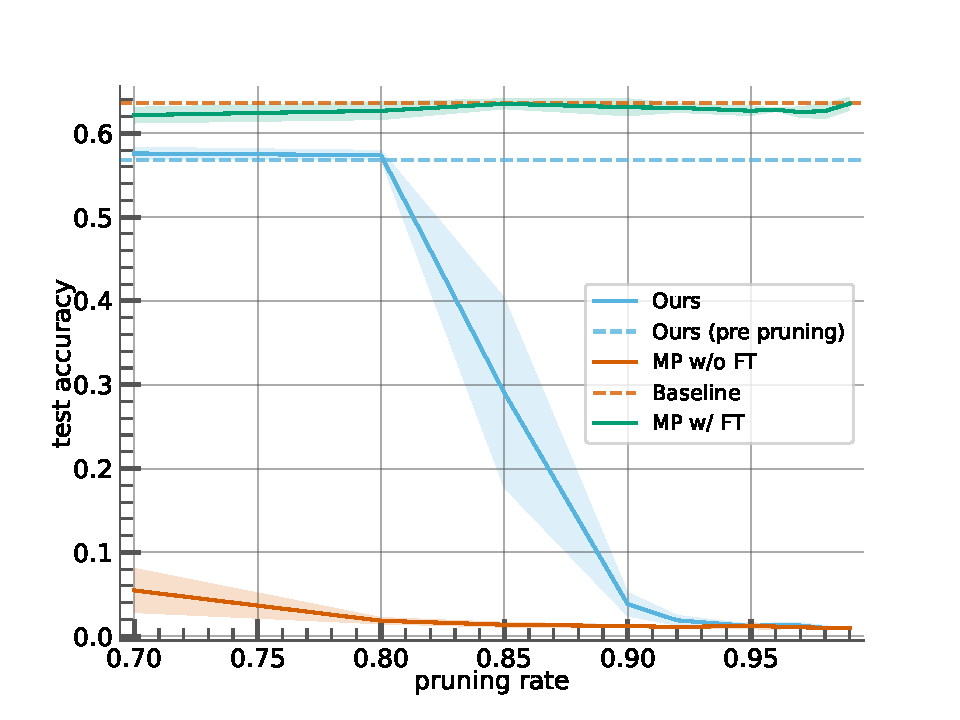
\includegraphics[width=0.49\linewidth]{chapter_1/assets/reparam_vs_mpft_PrunableResNet20_cifar100.pdf}}
  \\
  \subfloat[ResNet20 - CIFAR-10 (Number of Epochs)\label{fig:chap1:reparam_vs_mpft_resnet20_cifar10_epochs}  ]{
    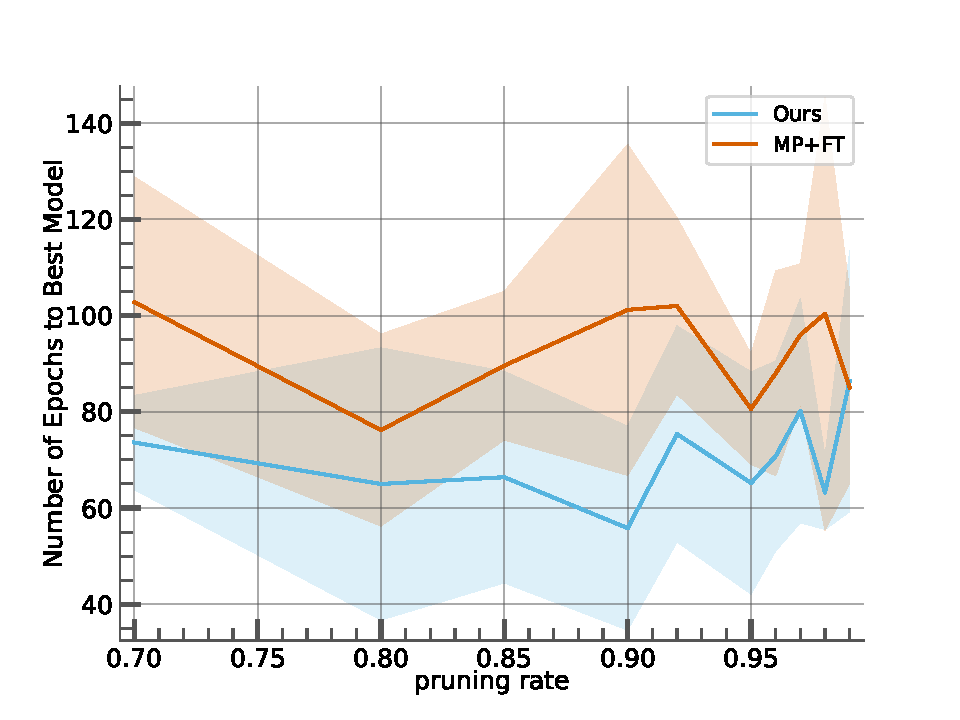
\includegraphics[width=0.49\linewidth]{chapter_1/assets/reparam_vs_mpft_training_time_PrunableResNet20_cifar10.pdf}}
  \subfloat[ResNet20 - CIFAR-100 (Number of Epochs)\label{fig:chap1:reparam_vs_mpft_resnet20_cifar100_epochs}]{
    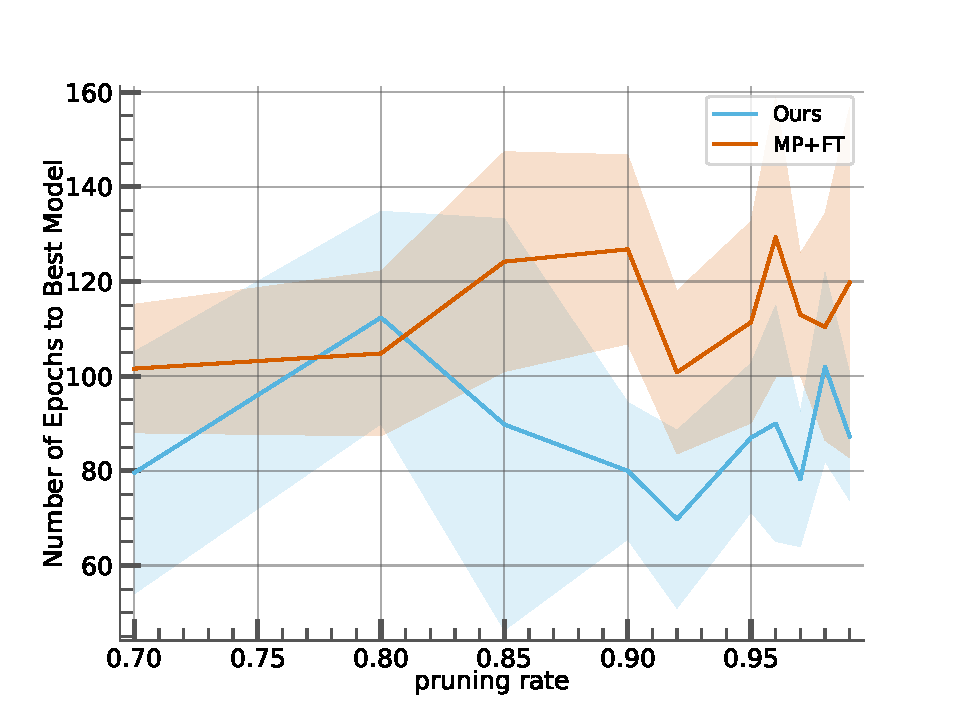
\includegraphics[width=0.49\linewidth]{chapter_1/assets/reparam_vs_mpft_training_time_PrunableResNet20_cifar100.pdf}}
  \caption{ Performances comparison of our method \em{(Ours)} against
    magnitude pruning with fine-tuning \em{(MP+FT)} with a ResNet20 network on
    CIFAR-10 and CIFAR-100 datasets, for different pruning rates.
    \Cref{fig:chap1:reparam_vs_mpft_resnet20_cifar10} and
    \cref{fig:chap1:reparam_vs_mpft_resnet20_cifar100} show the
    testing accuracy of the model and
    \cref{fig:chap1:reparam_vs_mpft_resnet20_cifar10_epochs} and
    \cref{fig:chap1:reparam_vs_mpft_resnet20_cifar100_epochs}
    the number of epochs needed to obtain the best model. Best viewed in colours.}
  \label{fig:chap1:reparam_vs_mpft_resnet20}
\end{figure}


\begin{figure}
  \centering
  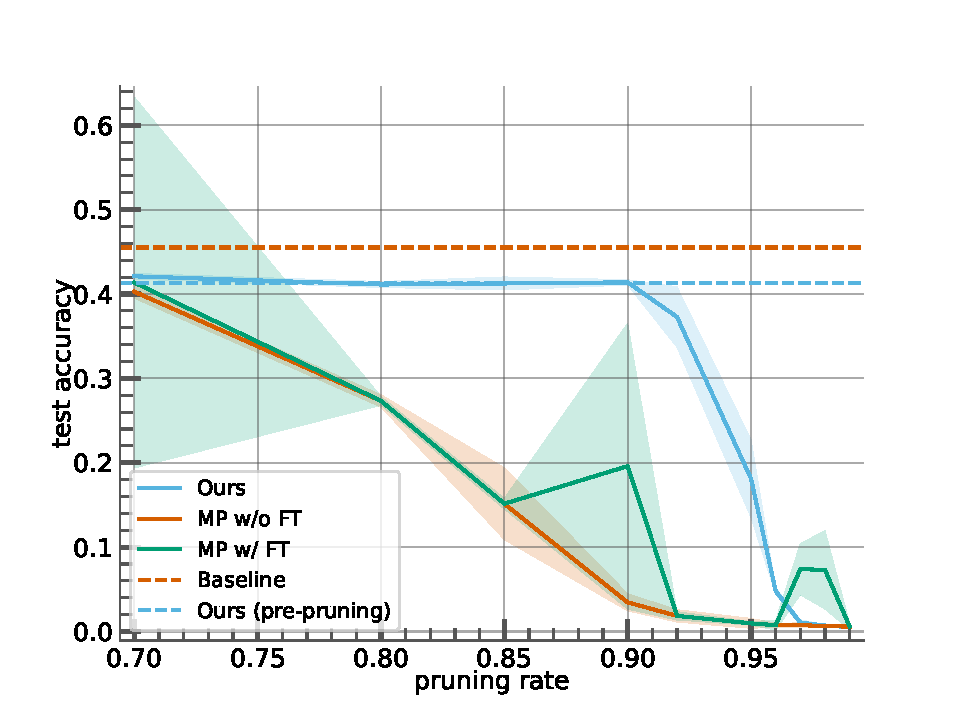
\includegraphics[width=0.49\textwidth]{chapter_1/assets/reparam_vs_mpft_PrunableResNet18_tinyimagenet.pdf}
  \caption{Performances comparison of our method \em{(Ours)} against
    magnitude pruning with fine-tuning \em{(MP+FT)} with a ResNet18 network on
    TinyImageNet dataset, for different pruning rates.}
  \label{fig:chap1:reparam_vs_mpft_resnet18}
\end{figure}

% endregion: perfs_figures

% endregion: performances

\subsection{Optimal Value of \texorpdfstring{$\lambda$}{Lambda}}
\label{sec:chap1:impact_of_lambda}

% region: lambda value

Our method relies on a budget loss whose relative importance compared to the
main task loss is controlled by a parameter $\lambda$ (cf.
\cref{eqn:chap1:globalloss}). The choice of this parameter is crucial to ensure
a good tradeoff between \emph{(i)} adhering to the budget constraint, which
ensures that the weights set to zero during the effective pruning step are
already vanishingly small if the constraint is satisfied. This implies that
zeroing these weights will have a minimal impact on performance; and \emph{(ii)}
the optimisation of the main task loss, which directly impacts the final
performance. The achieved budget as a function of the parameter $\lambda$ is
shown for different pruning rates in
\cref{fig:chap1:lambda_impact_pruning_90,fig:chap1:lambda_impact_pruning_95,fig:chap1:lambda_impact_pruning_99}.
In these figures, the achieved budget is computed as the sum of the weight
reparametrisations divided by the number of weights in the original network.\\

For low pruning rates (\cref{fig:chap1:lambda_impact_pruning_90}), a relatively
low value of $\lambda$ does not guarantee adherence to the budget constraint and
the final network has a smaller achieved budget than the targeted one.
Similarly, for higher pruning rates (\cref{fig:chap1:lambda_impact_pruning_99}),
a low value of $\lambda$ results in a budget in excess compared to the targeted
one. In both cases, the performances of networks trained with a low value of
$\lambda$ are subpar compared to higher values, as reported in
\cref{tab:chap1:lambda_impact}. In contrast to low values of $\lambda$, high
values might lay too much emphasis on the budget loss, and the network
performances are negatively impacted, even though the budget is satisfied or
almost satisfied. This is especially the case for a pruning rate of 95\%
associated with $\lambda=500$ and also for a pruning rate of 99\% for values of
$\lambda \geq 50$. Following the abovementioned observations, we set the value
of $\lambda$ to 5 for all the experiments. This value strikes the best balance
between the two objectives: budget loss and main task loss. Note that various
scheduling for $\lambda$ have been considered, but they do not significantly
improve performance (see \cref{sec:appendix:annihilation}).

% region: lambda_impact_figures

\begin{figure}
  \centering
  \subfloat[Pruning 90\% of the weights\label{fig:chap1:lambda_impact_pruning_90}]{
    
\includegraphics[width=0.49\linewidth]{chapter_1/assets/lambda_impact_pr_90_C4_CIFAR10.pdf}}
  \subfloat[Pruning 95\% of the weights\label{fig:chap1:lambda_impact_pruning_95}]{
    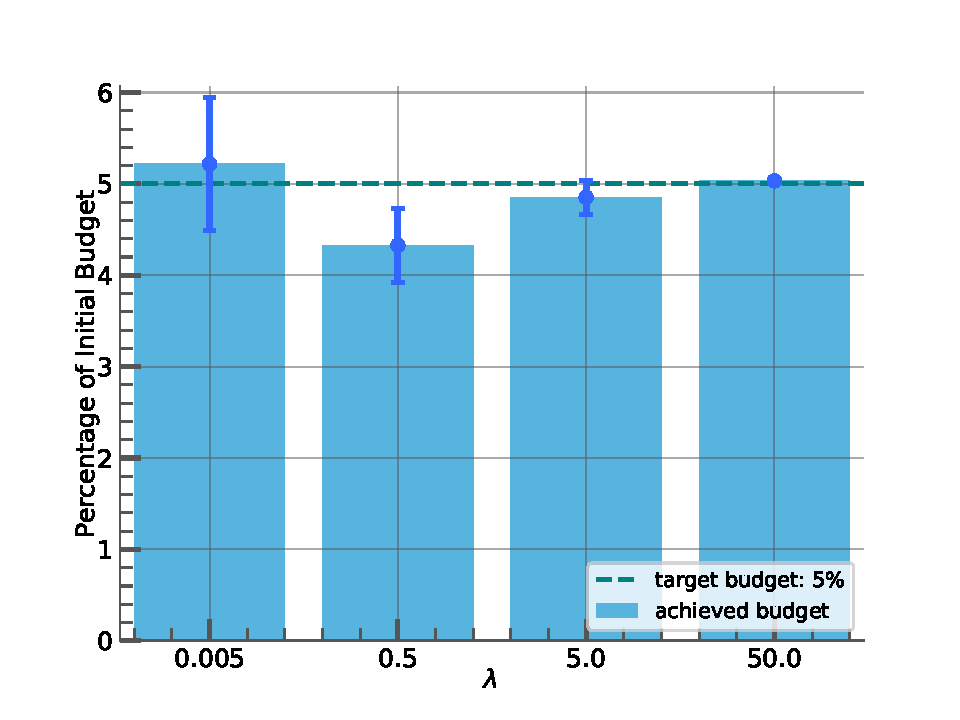
\includegraphics[width=0.49\linewidth]{chapter_1/assets/lambda_impact_pr_95_C4_CIFAR10.pdf}}
  \\
  \subfloat[Pruning 99\% of the weights\label{fig:chap1:lambda_impact_pruning_99}]{
    
\includegraphics[width=0.49\linewidth]{chapter_1/assets/lambda_impact_pr_99_C4_CIFAR10.pdf}}
  \caption{ Impact of the parameter $\lambda$ on the achieved final
    budget for a Conv4 network on CIFAR-10 dataset, for various pruning rates. A
    too-small value of $\lambda$ does not make the actual budget match the desired
    budget. The actual budget is either too small
    (\cref{fig:chap1:lambda_impact_pruning_90}) or too high
    (\cref{fig:chap1:lambda_impact_pruning_99}) compared to the target, depending
    on the applied pruning rate.}
  \label{fig:chap1:lambda_impact}
\end{figure}


\begin{table}[tbp]
  \centering
  \begin{center}
    \begin{tabular}{llcc}
      \toprule
      \textbf{Pruning Rate} (\%) & \textbf{$\lambda$}                         & \textbf{Achieved Budget} (\%)
                                 & \textbf{Test Accuracy (post pruning)} (\%)                                                             \\
      \midrule
      \multirow{5}{*}{90}        & 0.005                                      & 5.25 $\pm$ 0.69               & 85.83 $\pm$ 0.83          \\
                                 & 0.5                                        & 8.06 $\pm$ 0.19               & 86.34 $\pm$ 0.64          \\
                                 & 5                                          & 9.93 $\pm$ 0.03               & 85.82 $\pm$ 0.74          \\
                                 & 50                                         & \textbf{10.00 $\pm$ 0.01}     & \textbf{86.52 $\pm$ 0.46} \\
                                 & 500                                        & 10.03 $\pm$ 0.00              & 85.55 $\pm$ 0.49          \\
      \midrule
      \multirow{5}{*}{95}        & 0.005                                      & 5.22 $\pm$ 0.73               & \textbf{86.27 $\pm$ 0.32} \\
                                 & 0.5                                        & 4.33 $\pm$ 0.41               & 85.66 $\pm$ 0.74          \\
                                 & 5                                          & 4.85 $\pm$ 0.19               & 86.11 $\pm$ 0.48          \\
                                 & 50                                         & 5.03 $\pm$ 0.02               & 85.37 $\pm$ 0.37          \\
                                 & 500                                        & \textbf{5.00 $\pm$ 0.00}      & 10.00 $\pm$ 0.00          \\
      \midrule
      \multirow{5}{*}{99}        & 0.005                                      & 4.60 $\pm$ 0.29               & 40.52 $\pm$ 5.27          \\
                                 & 0.5                                        & 3.69 $\pm$ 0.38               & 42.45 $\pm$ 9.02          \\
                                 & 5                                          & 1.89 $\pm$ 0.45               & \textbf{76.85 $\pm$ 6.34} \\
                                 & 50                                         & \textbf{2.09 $\pm$ 0.15}      & 10.00 $\pm$ 0.00          \\
                                 & 500                                        & 2.28 $\pm$ 0.01               & 10.00 $\pm$ 0.00          \\
      \bottomrule
    \end{tabular}
  \end{center}
  \caption{
    Impact of the parameter $\lambda$ on the achieved budget and the post-pruning test accuracy of the model for a Conv4 network on the CIFAR-10 dataset
    for various pruning rates. Although a high value of $\lambda$ ensures
    the targeted budget is reached, it also leads to a lower test accuracy when
    the pruning rate increases.}
  \label{tab:chap1:lambda_impact}
\end{table}

% endregion: lambda_impact_figures

% endregion: lambda value

\subsection{Validation of the Budget Loss}
\label{sec:chap1:impact_of_budget_loss}

% region: budget impact

In order to establish the importance and the effectiveness of the budget loss in our
method, we present in this section the results of a comparative experimental
analysis with alternative variants.  Specifically, we investigated the impact of
the budget loss by comparing it with two other variants: \emph{(i)} a variant
where the budget loss is removed, and \emph{(ii)} a variant where the budget
loss is replaced with a regularisation loss based on the $\ell_1$ norm of the
network weights. In order to remove the budget loss, the value of $\lambda$ is set to
zero 0 in \cref{eqn:chap1:globalloss}. In the second variant, we varied the
mixing coefficient $\lambda$ between 0.1 and 100. Considering the same issue of
loss conditioning as in \cref{sec:chap1:budget_loss}, the $\ell_1$ norm is divided
by the total number of parameters, denoted $N$, before being added to the global loss. This
specific global loss is expressed as:

\begin{equation}
  \label{eqn:chap1:globalloss_l1}
  \mathcal{L} = \mathcal{L}_{task} + \lambda \cdot \frac{1}{N} \sum_{\ell=1}^{L} || \mathbf{w}_\ell ||_1
\end{equation}

Where $||~.~||_1$ represents the $\ell_1$. Values of $N$ for most of the used
architectures are reported in \cref{tab:dlo:networks_size}.\\

In both variants, the reparametrisation is kept in order to isolate the impact
of the budget loss. We evaluated the performance of our approach and the two
variants on the CIFAR-10 and CIFAR-100 datasets using Conv4, VGG16, and ResNet20
networks. The results are presented in
\cref{fig:chap1:no_budget_conv4,fig:chap1:no_budget_resnet20,fig:chap1:no_budget_vgg16}.
In the figures mentioned above, the variant without the budget loss is denoted
\emph{w/o budget}, and the variant with a $\ell_1$ regularisation loss is
referred to as \emph{$\ell_1$ reg.}. The results denoted \emph{w/ budget}
represents our method in the same setup as in \cref{sec:chap1:performances}.\\

Removing the budget loss (variant \emph{(i)} - \emph{w/o budget}) negatively
impacts the network performances. The test accuracy is systematically lower than
the one obtained with the budget loss. This is particularly visible in
\cref{fig:chap1:no_budget_conv4_cifar100,fig:chap1:no_budget_vgg16_cifar100}.
Removing the budget loss does not push the optimisation to introduce sparsity,
let alone to respect the targeted budget. Since sparsity was not introduced
beforehand, the effective pruning step has a negative impact on the network
performance. Indeed, the latter was not trained with a prior on either targeted
sparsity or targeted budget, embedded in the loss.\\


Replacing the budget loss with a $\ell_1$ regularisation loss (variant
\emph{(ii)} - \emph{$\ell_1$ reg.}) also impacts negatively the performance,
with the exception of the ResNet20 network
(\cref{fig:chap1:no_budget_resnet20}). Although performances are generally worse
than our method (\emph{w/ budget}), results indicate that the mixing coefficient
$\lambda$ has major importance. Indeed, the $\ell_1$ regularisation does not
target a precise budget, however, it still helps optimisation to introduce
sparsity in the network. Thus, for certain pruning rates, the variant
\emph{(ii)} can exhibit better results than our method (especially visible on
\cref{fig:chap1:no_budget_resnet20_cifar10,fig:chap1:no_budget_resnet20_cifar100}).
Nevertheless, the choice of $\lambda$ is critical and not trivial. Because of
the absence of a budget loss, the optimisation does not take any targeted level
of sparsity into account. The tradeoff between optimising the main task loss and
the $\ell_1$ regularisation loss is controlled only by the parameter $\lambda$,
which makes it difficult to find a single value suited for a large range of
pruning rates, networks and datasets. Since variant \emph{(ii)} does not target
any specific sparsity, in
\cref{fig:chap1:no_budget_conv4,fig:chap1:no_budget_vgg16,fig:chap1:no_budget_resnet20},
we vary the pruning rate to examine the performance of trained networks at
various sparsity levels.\\

In contrast, our method is able to achieve good performance across multiple and
diverse conditions, without the need to try different \DIFdelbegin \DIFdel{value }\DIFdelend \DIFaddbegin \DIFadd{values }\DIFaddend of $\lambda$.
Experiments presented in this section reveal that the budget loss is a critical
component of the method to train networks and prune them while introducing a
minimal impact on the performance if no fine-tuning is applied. While the
$\ell_1$ regularisation loss may achieve superior performance in certain cases,
our method is simpler to implement since it does need to search for a value of
$\lambda$ per architecture, and more robust in its applicability across various
scenarios.\\

% region: no budget
\begin{figure}
  \centering
  \subfloat[Conv4 CIFAR-10\label{fig:chap1:no_budget_conv4_cifar10}]{
    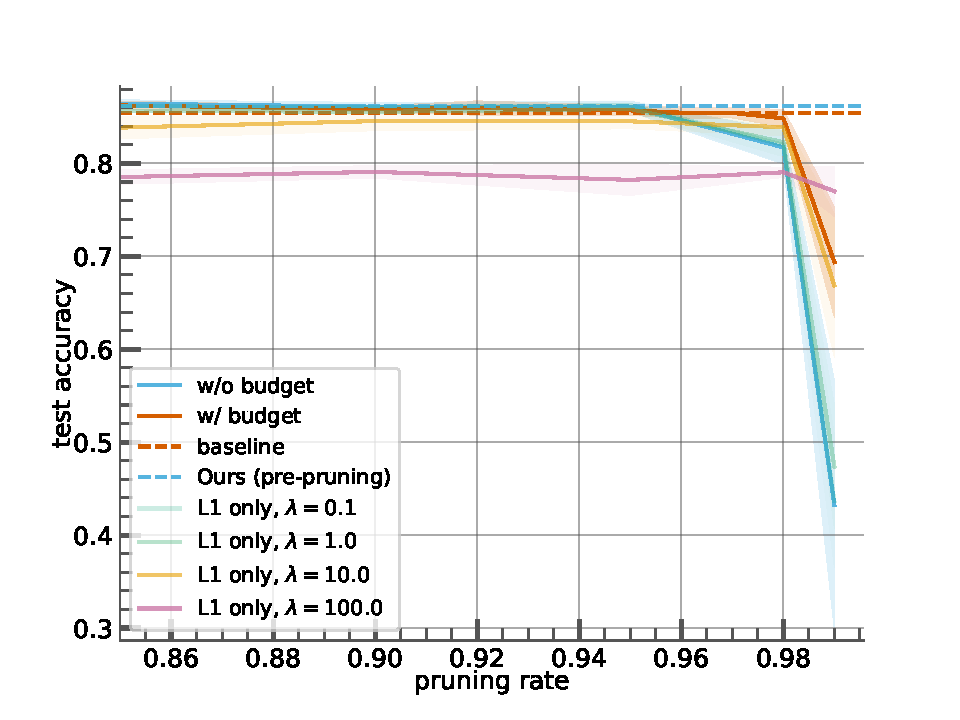
\includegraphics[width=0.49\textwidth]{chapter_1/assets/ours_vs_no_lambda_vs_l1_only_cifar10_Conv4.pdf}}
    \subfloat[Conv4 CIFAR-100\label{fig:chap1:no_budget_conv4_cifar100}]{
    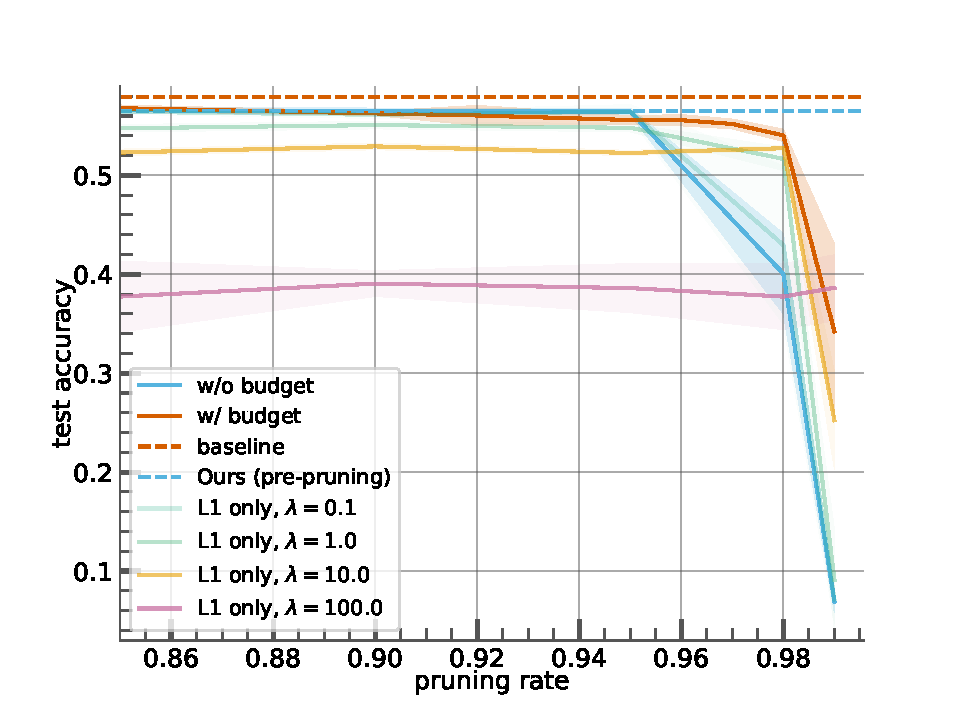
\includegraphics[width=0.49\textwidth]{chapter_1/assets/ours_vs_no_lambda_vs_l1_only_cifar100_Conv4.pdf}}
    \caption{ Comparison of our method and its variant without the budget loss.
    The experimental results are referred to as \emph{$\ell_1$ reg.}, wherein
    the budget loss is replaced by a $\ell_1$ regularisation loss on the network
    weights. The mixing coefficient $\lambda$ is varied from 0.1 to 100,
    depending on the experiment. \emph{w/o budget} corresponds to the absence of
    the budget loss (this is equivalent to $\lambda = 0$). On the other hand,
    \emph{w/ budget} corresponds to our method, with the same setup as described
    in \cref{sec:chap1:performances}. Results are presented for a Conv4 network,
    trained on CIFAR-10 (\cref{fig:chap1:no_budget_conv4_cifar10}) and CIFAR-100
    (\cref{fig:chap1:no_budget_conv4_cifar100}). Best viewed in colours.}
  \label{fig:chap1:no_budget_conv4}
\end{figure}



\begin{figure}
  \centering
  \subfloat[ResNet20 CIFAR-10\label{fig:chap1:no_budget_resnet20_cifar10}]{
    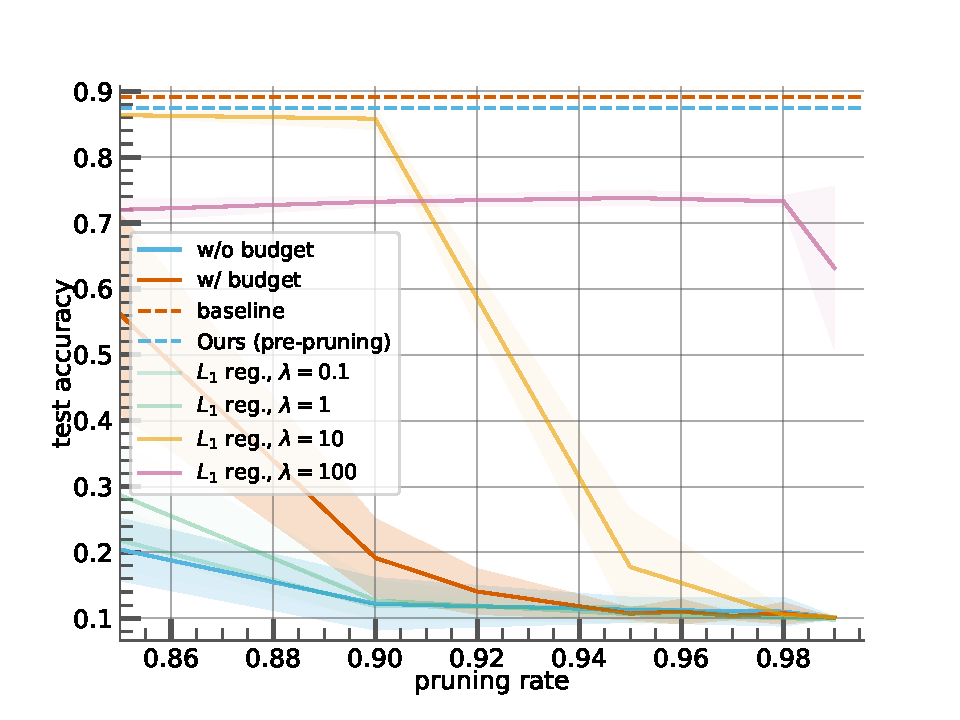
\includegraphics[width=0.49\textwidth]{chapter_1/assets/ours_vs_no_lambda_vs_l1_only_cifar10_PrunableResNet20.pdf}}
    \subfloat[ResNet20 CIFAR-100\label{fig:chap1:no_budget_resnet20_cifar100}]{
    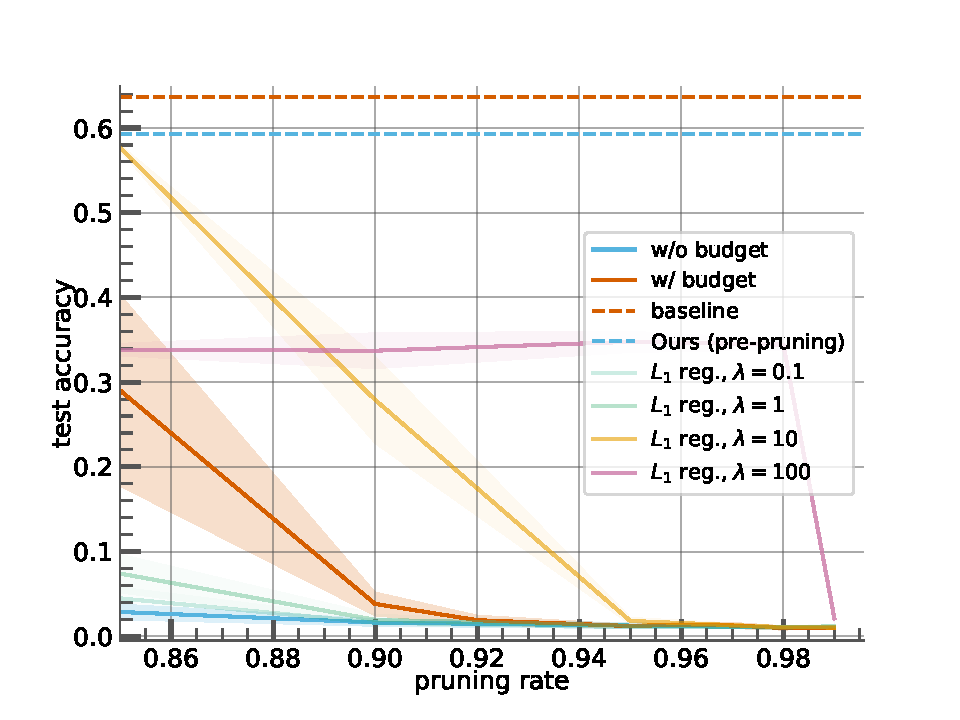
\includegraphics[width=0.49\textwidth]{chapter_1/assets/ours_vs_no_lambda_vs_l1_only_cifar100_PrunableResNet20.pdf}}
    \caption{ Comparison of our method and its variant without the budget loss.
    The experimental results are referred to as \emph{$\ell_1$ reg.}, wherein
    the budget loss is replaced by a $\ell_1$ regularisation loss on the network
    weights. The mixing coefficient $\lambda$ is varied from 0.1 to 100,
    depending on the experiment. \emph{w/o budget} corresponds to the absence of
    the budget loss (this is equivalent to $\lambda = 0$). On the other hand,
    \emph{w/ budget} corresponds to our method, with the same setup as described
    in \cref{sec:chap1:performances}. Results are presented for a ResNet20
    network, trained on CIFAR-10 (\cref{fig:chap1:no_budget_resnet20_cifar10})
    and CIFAR-100 (\cref{fig:chap1:no_budget_resnet20_cifar100}). Best viewed in
    colours.}
  \label{fig:chap1:no_budget_resnet20}
\end{figure}



\begin{figure}
  \centering
  \subfloat[VGG16 CIFAR-10\label{fig:chap1:no_budget_vgg16_cifar10}]{
    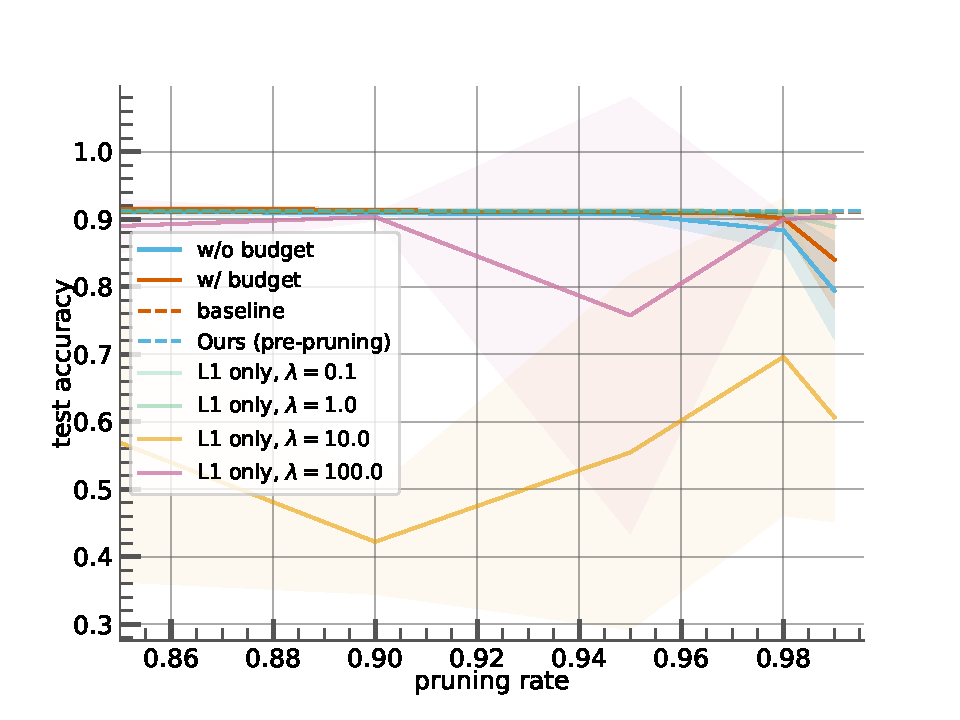
\includegraphics[width=0.49\textwidth]{chapter_1/assets/ours_vs_no_lambda_vs_l1_only_cifar10_PrunableVGG16.pdf}}
    \subfloat[VGG16 CIFAR-100\label{fig:chap1:no_budget_vgg16_cifar100}]{
    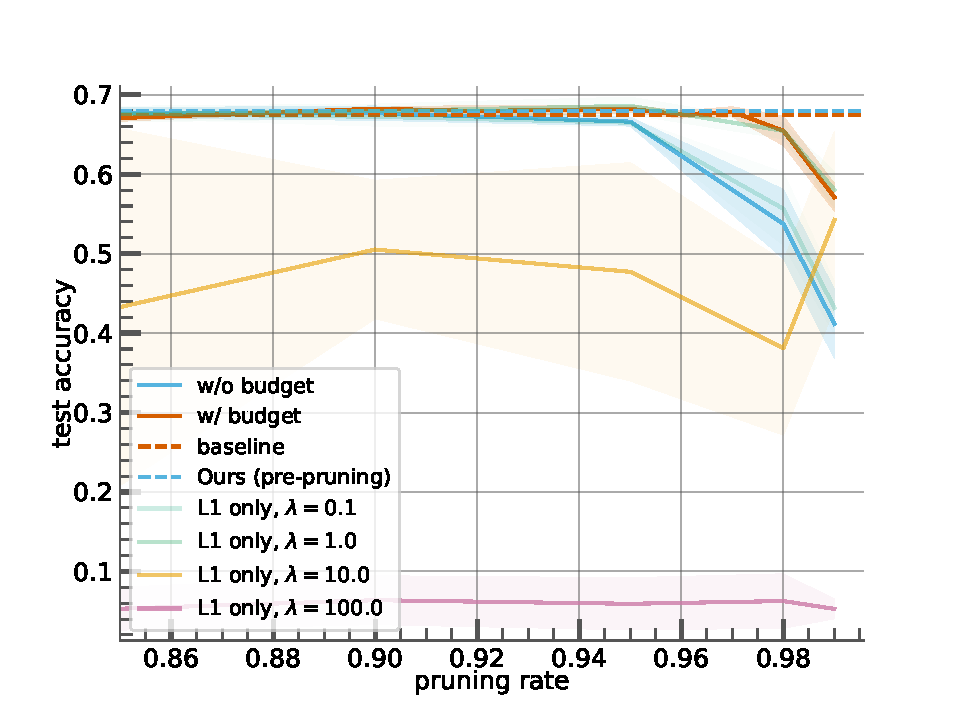
\includegraphics[width=0.49\textwidth]{chapter_1/assets/ours_vs_no_lambda_vs_l1_only_cifar100_PrunableVGG16.pdf}}
    \caption{ Comparison of our method and its variant without the budget loss.
    The experimental results are referred to as \emph{$\ell_1$ reg.}, wherein
    the budget loss is replaced by a $\ell_1$ regularisation loss on the network
    weights. The mixing coefficient $\lambda$ is varied from 0.1 to 100,
    depending on the experiment. \emph{w/o budget} corresponds to the absence of
    the budget loss (this is equivalent to $\lambda = 0$). On the other hand,
    \emph{w/ budget} corresponds to our method, with the same setup as described
    in \cref{sec:chap1:performances}. Results are presented for a VGG16 network,
    trained on CIFAR-10 (\cref{fig:chap1:no_budget_vgg16_cifar10}) and CIFAR-100
    (\cref{fig:chap1:no_budget_vgg16_cifar100}). Best viewed in colours.}
  \label{fig:chap1:no_budget_vgg16}
\end{figure}

% endregion: no budget

% endregion: budget impact

\subsection{Validation of the Reparametrisation}
\label{sec:chap1:impact_of_reparametrisation}

% region: reparam impact

The proposed method comprises two primary components: budget loss and weight
reparametrization. The previous section establishes the significance of the
budget loss in achieving optimal performance. In this section, we study the
impact of incorporating weight reparametrisation. To establish the necessity of
weight reparametrisation, we compare our approach with a variant where the
budget loss is applied but the weight reparametrisation is not. This variant is
denoted \emph{budget only} in the following. The objective of this variant and
the comparison is to isolate the impact of weight reparametrization. The budget
loss is evaluated in the same way as described in \cref{sec:chap1:budget_loss}.
Note that in the \emph{budget only} variant the budget evaluation uses our
reparametrisation function as a surrogate $\ell_0$ norm but the weights used to
poduce the network output are the standard weights $\mathbf{w}$, not the
reparametrised weights $\mathbf{\hat{w}}$.\\

We evaluate the performance of our method and the \emph{budget only} variant on
Conv4, ResNet20, and VGG16 networks using CIFAR-10 and CIFAR-100 datasets (see
\cref{fig:chap1:budget_only_conv4,fig:chap1:budget_only_resnet20,fig:chap1:budget_only_vgg16}).
Both the proposed approach and \emph{budget only} variant are trained with the
same hyperparameters, namely, the learning rate, weight decay, number of epochs
and the \emph{Reduce on Plateau} policy for the learning rate. For the
\textit{budget only} variant,  we perform experiments by varying the mixing
coefficient $\lambda$ from 0.5 to 500. The performances did not vary
significantly w.r.t. $\lambda$, suggesting that the mixing coefficient does not
have a significant impact on the performance. Therefore, in order to ensure the
clarity of
\cref{fig:chap1:budget_only_conv4,fig:chap1:budget_only_resnet20,fig:chap1:budget_only_vgg16},
we only display the results for $\lambda = 5$.\\

\Cref{fig:chap1:budget_only_conv4,fig:chap1:budget_only_resnet20,fig:chap1:budget_only_vgg16}
present the results of the performance comparison. Our method is referred to as
\emph{budget + reparam} and is evaluated after pruning, whereas the \emph{budget
only} variant results are presented both before and after pruning. On Conv4 and
VGG16 (\cref{fig:chap1:budget_only_conv4,fig:chap1:budget_only_vgg16},
respectively), our method performs on par with the \emph{budget only} variant
before pruning while being already pruned, up to very high pruning rates (more
than 98\%). On the contrary, and even for ResNet20, the \emph{budget only}
post-pruning variant performs poorly. The \emph{budget only} variant performance
is massively impaired by the \emph{effective pruning} step, even though the
budget is thoroughly respected (\cref{tab:chap1:impact_of_reparametrisation}).
In comparison, our method performs much better than the latter when
\textit{effective pruning} is applied to both methods. The budget loss alone
enforces a stricter adherence to the targeted budget
(\cref{tab:chap1:impact_of_reparametrisation}), however, the lack of
reparametrisation fails to prepare the network for the \emph{effective pruning}
step. Indeed, weights are not soft-pruned and the network is not prepared for
sparsity.\\

% region: table budget only
\begin{table}
  \centering
  \begin{tabular}{lllc}
    \toprule
    \textbf{Dataset}          & \textbf{Network}          & \textbf{Pruning Rate} (\%) &
    \textbf{Achieved Budget} (\%)                                                                         \\
    \midrule
    \multirow{9}{*}{CIFAR-10}  & \multirow{3}{*}{Conv4}    & 90                         & 9.99 $\pm$ 0.00  \\
                              &                           & 95                         & 4.97 $\pm$ 0.01  \\
                              &                           & 99                         & 0.98 $\pm$ 0.00  \\
    \cline{2-4}
                              & \multirow{3}{*}{ResNet20} & 90                         & 9.83 $\pm$ 0.02  \\
                              &                           & 95                         & 4.88 $\pm$ 0.01  \\
                              &                           & 99                         & 0.98 $\pm$ 0.00  \\
    \cline{2-4}

                              & \multirow{3}{*}{VGG16}    & 90                         & 10.00 $\pm$ 0.00 \\
                              &                           & 95                         & 5.00 $\pm$ 0.00  \\
                              &                           & 99                         & 1.00 $\pm$ 0.00  \\
    \midrule
    \multirow{9}{*}{CIFAR-100} & \multirow{3}{*}{Conv4}    & 90                         & 9.94 $\pm$ 0.02  \\
                              &                           & 95                         & 4.91 $\pm$ 0.02  \\
                              &                           & 99                         & 0.98 $\pm$ 0.00  \\
    \cline{2-4}

                              & \multirow{3}{*}{ResNet20} & 90                         & 9.84 $\pm$ 0.02  \\
                              &                           & 95                         & 4.91 $\pm$ 0.01  \\
                              &                           & 99                         & 1.00 $\pm$ 0.00  \\
    \cline{2-4}

                              & \multirow{3}{*}{VGG16}    & 90                         & 10.00 $\pm$ 0.00 \\
                              &                           & 95                         & 5.00 $\pm$ 0.00  \\
                              &                           & 99                         & 1.00 $\pm$ 0.00  \\
    \bottomrule
  \end{tabular}
  \caption{Achieved budget for the \emph{budget only} variant. Results are
    presented for $\lambda=5$. Across all experiments, the achieved budget matches
    closely the targeted budget, which is computed as $1-$pruning
    rate.}
  \label{tab:chap1:impact_of_reparametrisation}
\end{table}


% endregion: table budget only

The results presented in this comparison and the one of
\cref{sec:chap1:budget_loss} show that both components of our method are of
crucial importance. In particular, the reparametrization allows for a
considerably better generalization of the network after pruning, thus enabling a
much higher level of performance.
\Cref{sec:chap1:impact_of_budget_loss,sec:chap1:impact_of_reparametrisation}
provide empirical evidence that no component of our method can be removed
without significant impairment of the performance, and therefore, they
function in synergy.

% region: budget only

\begin{figure}
  \centering
  \subfloat[Conv4 CIFAR-10\label{fig:chap1:budget_only_conv4_cifar10}]{
    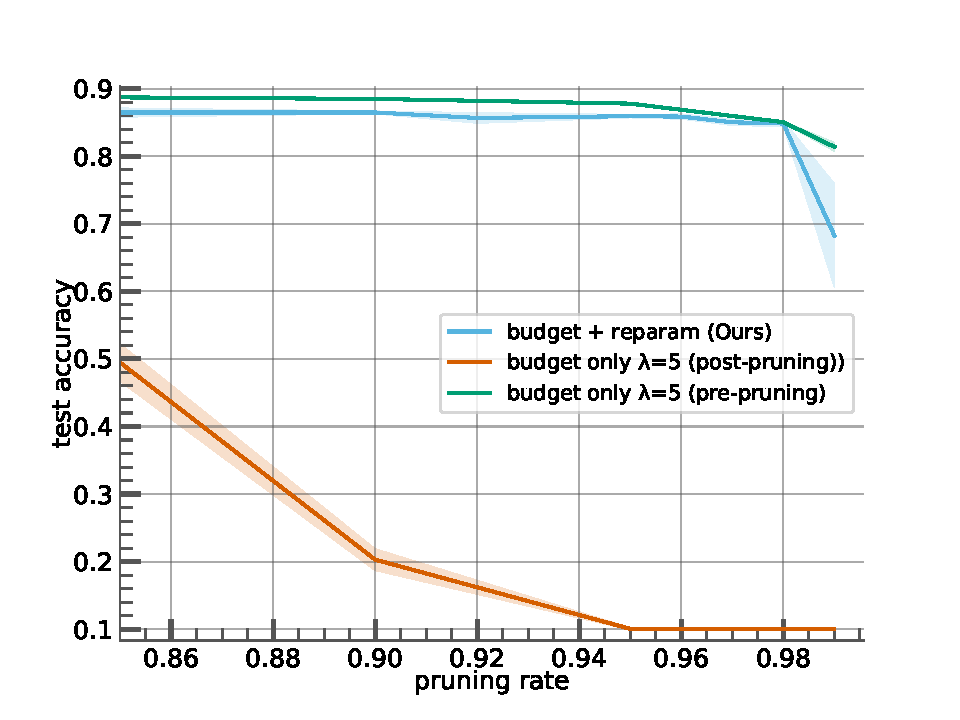
\includegraphics[width=0.49\textwidth]{chapter_1/assets/budget_only_cifar10_Conv4.pdf}}
  \subfloat[Conv4 CIFAR-100\label{fig:chap1:budget_only_conv4_cifar100}]{
    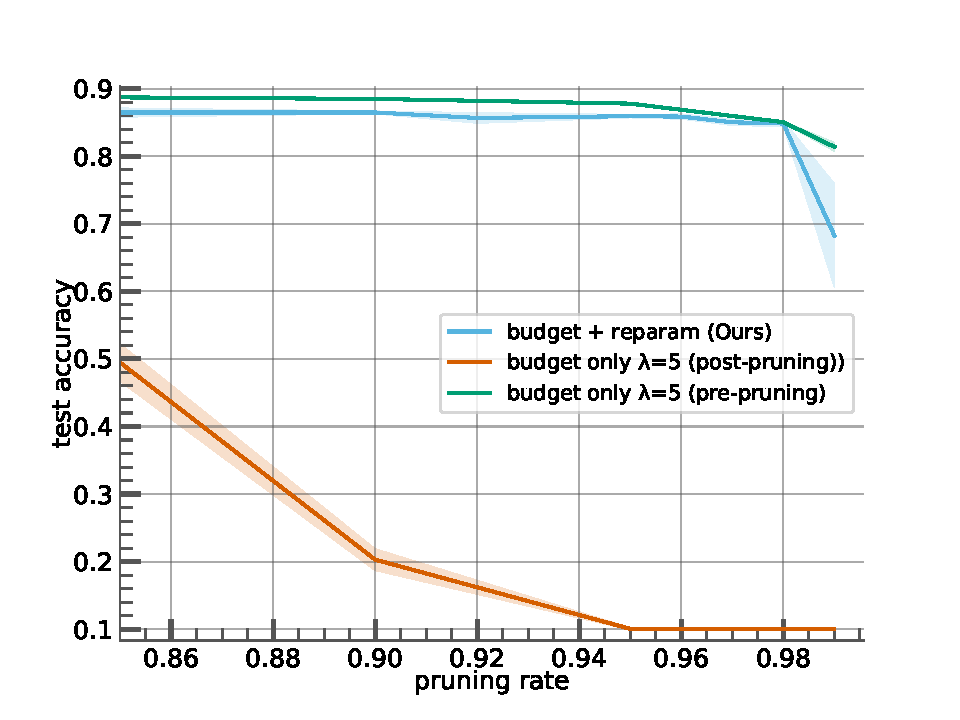
\includegraphics[width=0.49\textwidth]{chapter_1/assets/budget_only_cifar10_Conv4.pdf}}
  \caption{Comparison of our method and its variant without the
    reparametrization on Conv4, evaluated on CIFAR-10 and CIFAR-100. Our method
    (\emph{budget + reparam}) has similar performance to the \emph{budget only}
    variant before pruning, whereas our method, is already pruned. Once pruned,
    the \emph{budget only} variant is significantly impaired.}
  \label{fig:chap1:budget_only_conv4}
\end{figure}

\begin{figure}
  \centering
  \subfloat[ResNet20 CIFAR-10\label{fig:chap1:budget_only_resnet20_cifar10}]{
    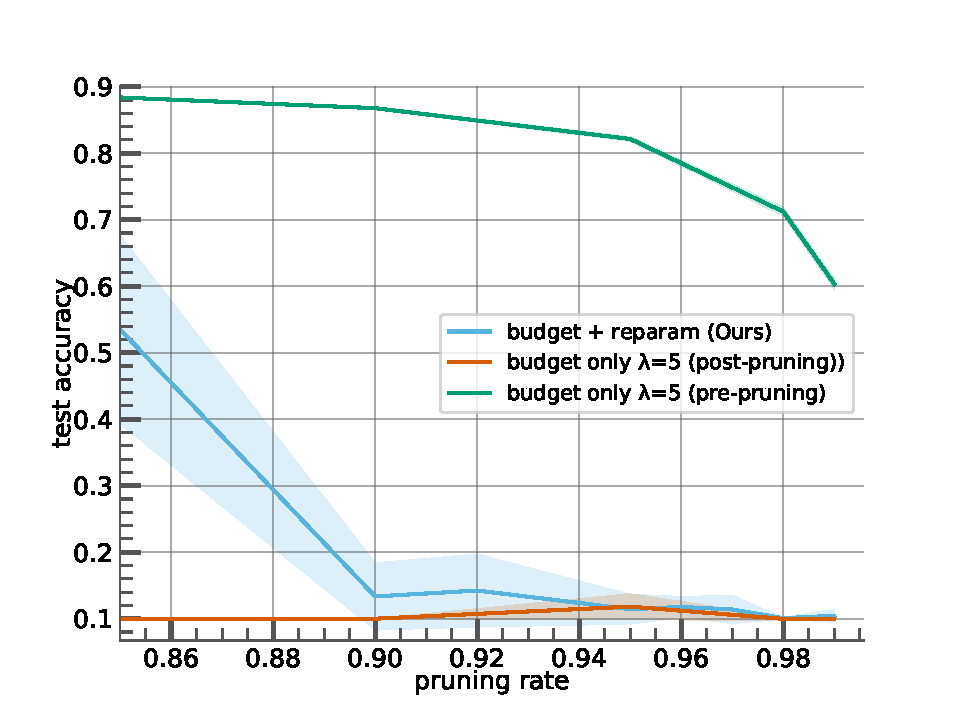
\includegraphics[width=0.49\textwidth]{chapter_1/assets/budget_only_cifar10_PrunableResNet20.pdf}}
  \subfloat[ResNet20 CIFAR-100\label{fig:chap1:budget_only_resnet20_cifar100}]{
    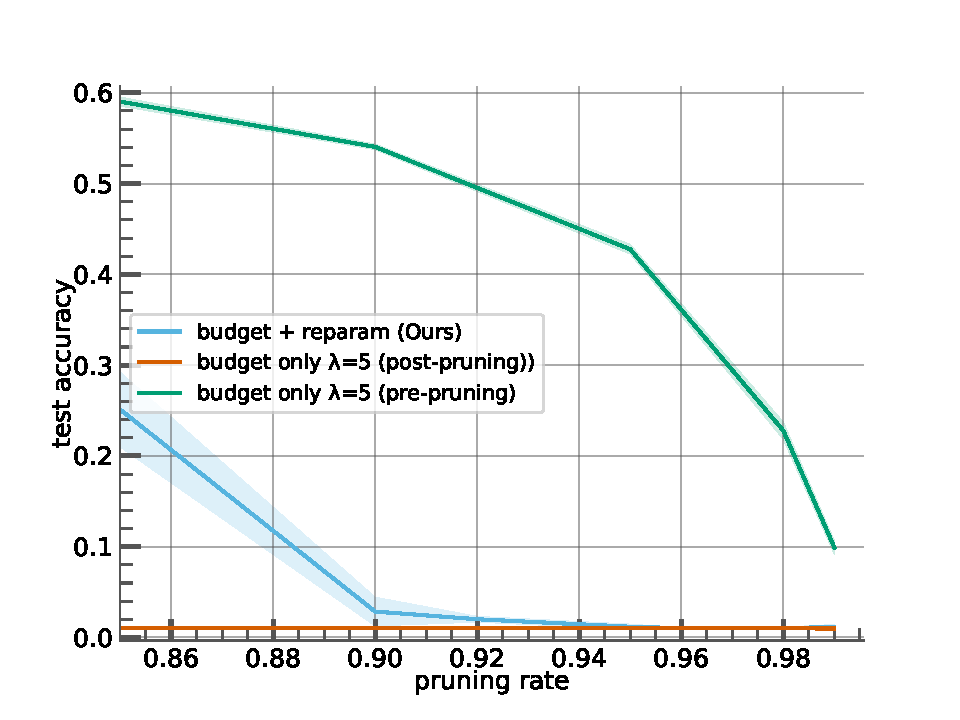
\includegraphics[width=0.49\textwidth]{chapter_1/assets/budget_only_cifar100_PrunableResNet20.pdf}}
  \caption{Comparison of our method and its variant without the
    reparametrization on ResNet20, evaluated on CIFAR-10 and CIFAR-100. Due to the
    small size of the network (see \cref{tab:dlo:networks_size}), the pruned
    version of our method (\emph{budget + reparam}) and the \emph{budget only}
    variant cannot keep up with the unpruned version. Nevertheless, if considering
    the pruned versions, our method scores better, thanks to the addition of the
    reparametrization.}
  \label{fig:chap1:budget_only_resnet20}
\end{figure}

\begin{figure}
  \centering
  \subfloat[VGG16 CIFAR-10\label{fig:chap1:budget_only_vgg6_cifar10}]{
    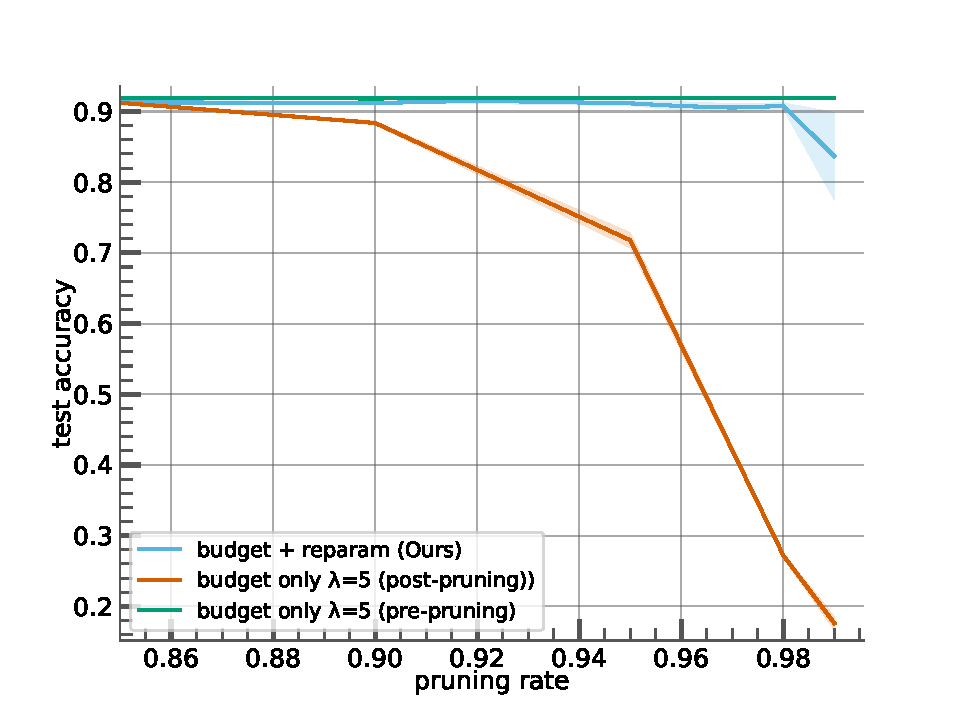
\includegraphics[width=0.49\textwidth]{chapter_1/assets/budget_only_cifar10_PrunableVGG16.pdf}}
  \subfloat[VGG16 CIFAR-100\label{fig:chap1:budget_only_vgg6_cifar100}]{
    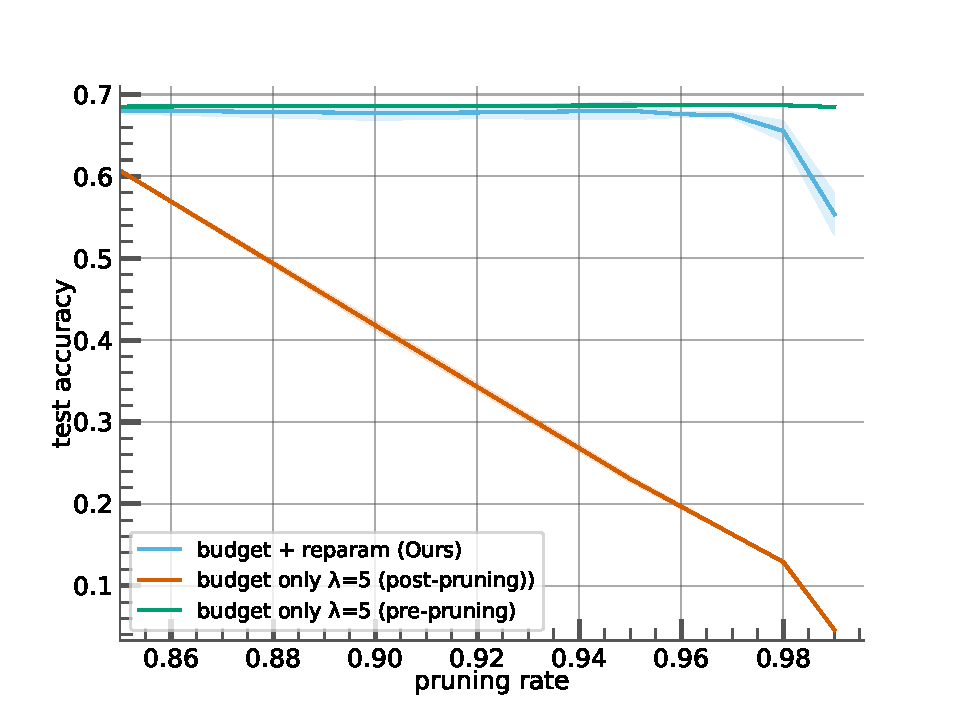
\includegraphics[width=0.49\textwidth]{chapter_1/assets/budget_only_cifar100_PrunableVGG16.pdf}}
  \caption{Comparison of our method and its variant without the
    reparametrizationn VGG16, evaluated on CIFAR-10 and CIFAR-100. Our method
    (\emph{budget + reparam}) has similar performance to the \emph{budget only}
    variant before pruning, whereas our method, is already pruned. Once pruned,
    the \emph{budget only} variant is significantly impaired.}
  \label{fig:chap1:budget_only_vgg16}
\end{figure}

% endregion: budget only

% endregion: reparam impact

\subsection{Tuned Initialisation}\label{sec:chap1:impact_of_fine_tuning}

% region : finetuning 

% Although the method presented in this chapter was designed to circumvent the
% need for fine-tuning, it can be used to fine-tune a network trained
% conventionally. 

In the previous sections, weights were initialised with the standard Kaiming
initialisation scheme \cite{DBLP:conf/iccv/HeZRS15} (see
\cref{sec:appendix:xavier_init}). In this section we study an alternative
initialisation scheme: we initialise the weights of the network with trained
and pruned weights. These weights are obtained by training the network in its
standard configuration (\emph{i.e.} without reparametrisation and budget loss)
up to convergence and then the weights are pruned with magnitude pruning at a
specified pruning rate. In other words, our method is used to fine-tune the
weights of a trained and pruned network. This \DIFdelbegin \DIFdel{fine-tunign }\DIFdelend \DIFaddbegin \DIFadd{fine-tuning }\DIFaddend setup is of particular
interest since the major deep learning frameworks
\cite{DBLP:conf/nips/PaszkeGMLBCKLGA19,DBLP:journals/corr/AbadiABBCCCDDDG16}
provides pretrained weights for various architectures \cite{pytorch_vision} but
it is up to the end user to prune and fine-tune them according to their needs.\\

We compare the performances of a network trained in a standard way, then pruned
with magnitude pruning and finally fine-tuned with two methods: Our method and
standard fine-tuning \cite{DBLP:conf/nips/HanPTD15}. Put simply, this section
describes a process where the initial weights of the network are not randomly
initialised, but are trained and pruned weights. Note that the pruning
\DIFdelbegin \DIFdel{definitly
}\DIFdelend \DIFaddbegin \DIFadd{definitely }\DIFaddend zeroes out the smallest magnitude weights and they are not
reactivated during the fine-tuning. The latter only \DIFdelbegin \DIFdel{tune }\DIFdelend \DIFaddbegin \DIFadd{tunes }\DIFaddend the remaining unpruned
weights. This setup is evaluated on Conv4, ResNet20 and VGG16 for both CIFAR-10
and CIFAR-100. The results are shown in
\cref{fig:chap1:finetuning_impact_conv4,fig:chap1:finetuning_impact_resnet20,fig:chap1:finetuning_impact_vgg6}.
First, a network is trained for 150 epochs on the main classification task. Then
it is pruned up to a specified pruning rate. The pruning criterion used is the
magnitude of the weights where weights with the smallest absolute \DIFdelbegin \DIFdel{value }\DIFdelend \DIFaddbegin \DIFadd{values }\DIFaddend are
removed in an unstructured way. The pruned network is then fine-tuned for 300
epochs with an early stopping criterion based on the validation accuracy. The
training is stopped prematurely if the validation accuracy does not improve for
30 epochs. When fine-tuned with our methods, the pruned network is treated as
the original network. The initial latent weights of our method ($\mathbf{w}$)
are the ones of the trained and pruned network. They are reparametrised as in
\ref{sec:chap1:weight_reparam}.\\

Except for results with the Conv4 networks, fine-tuning a network with our
method overperforms the conventional fine-tuning method by a comfortable margin
on ResNet20 across all pruning rates
(\cref{fig:chap1:finetuning_impact_resnet20}) and VGG16
(\cref{fig:chap1:finetuning_impact_vgg6}) for pruning rates higher than 96\%. At
initialisation, the weights of the network are already pruned to the targeted
pruning rate. With the enforcement of the budget through budget loss, the
remaining unpruned weights cannot dwindle to zero, hence preserving them during
the fine-tuning process. In contrast, in the absence of budget loss, the
remaining weight values are not restricted, allowing them to possibly vanish,
resulting in further a drop of network capacity with weights of vanishingly
small magnitude. This behaviour is highlighted by the following additional
experimental results displayed in
\cref{fig:chap1:finetuning_with_init_not_pruned}. This experiment involves a
comparison between two initial setups: one where the initial weights are only
fine-tuned and another where they are fine-tuned and then pruned. The outcomes
demonstrate that initialising a network with weights that are fine-tuned and
then pruned beforehand yields significantly superior results. Moreover, the
networks produced by fine-tuning with our method are much more consistent from
one run to another. This is illustrated by the standard deviation being so small
that the colored area around the solid line is barely visible on the graphs.
This is not the case for the conventional fine-tuning where performances vary
greatly from one run to another. This is especially visible in
\cref{fig:chap1:finetuning_impact_conv4_cifar10}.\\

Although the method proposed in this chapter was not initially intended for
fine-tuning networks, it demonstrates superior performance compared to
widely-used standard fine-tuning techniques. Notably, it exhibits enhanced
recovery from the performance decline that occurs following pruning.
Furthermore, the performance consistency of networks fine-tuned with our method
is significantly higher across multiple runs in comparison to networks generated
by traditional fine-tuning methods. The slight variation observed in the results
indicates increased robustness against the inherent randomness of the
optimization process. Consequently, the final performance is less dependent on
specific initializations, batch orders, or data augmentation seeds than with
standard fine-tuning approaches.\\

% region: fine-tuning figs

\begin{figure}
  \centering
  \subfloat[Conv4 CIFAR-10\label{fig:chap1:finetuning_impact_conv4_cifar10}]{
    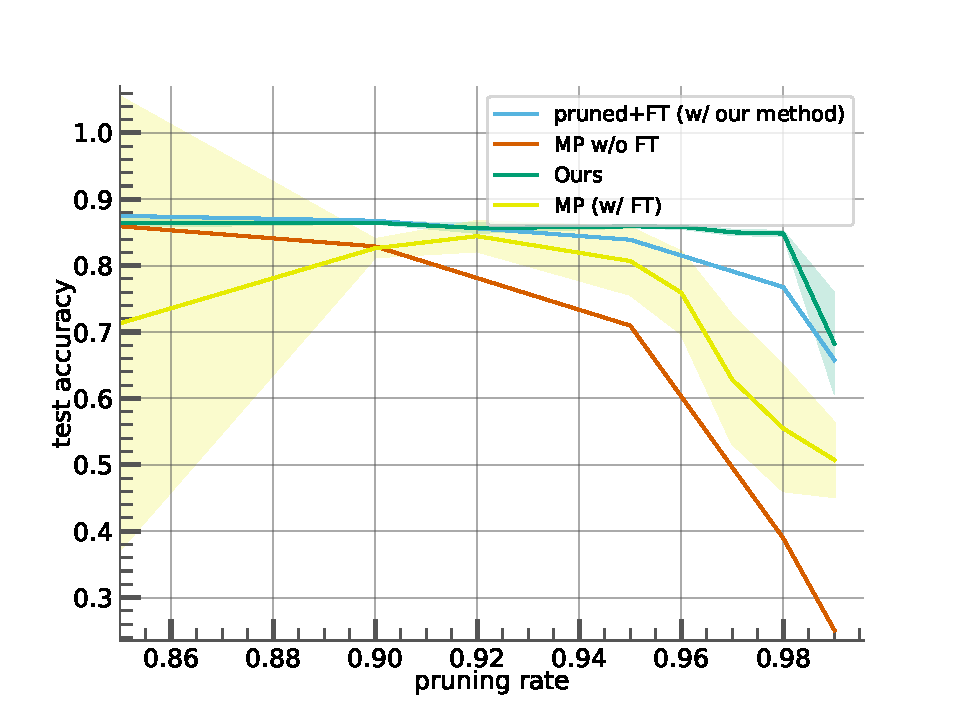
\includegraphics[width=0.49\textwidth]{chapter_1/assets/finetuning_cifar10_Conv4.pdf}}
  \subfloat[Conv4 CIFAR-100\label{fig:chap1:finetuning_impact_conv4_cifar100}]{
    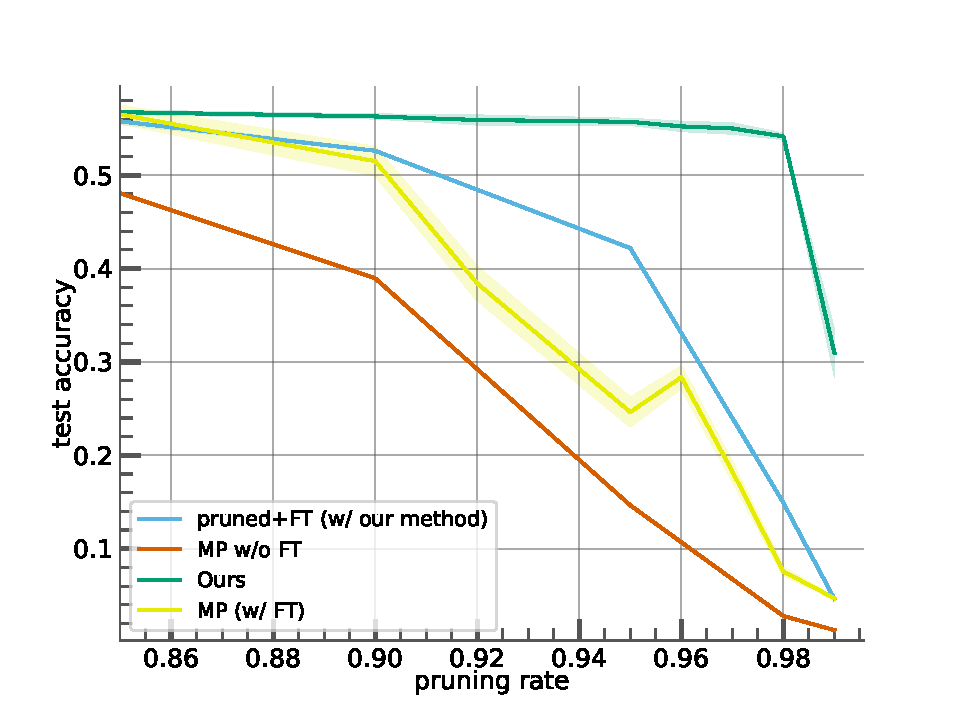
\includegraphics[width=0.49\textwidth]{chapter_1/assets/finetuning_cifar100_Conv4.pdf}}
  \caption{ Fine-tuning of a Conv4 network pruned by magnitude pruning (\emph{MP
      w/o FT}) on the CIFAR-10 and CIFAR-100 datasets for various pruning rates.
    Conventional (\emph{MP w/ FT}) fine-tuning is compared to fine-tuning with our
    method (\emph{pruned+FT (w/ our method)}). Our method, described in
    \cref{sec:chap1:overview}, is shown for comparison purposes (\emph{Ours}). On
    this network, our method performs better than other approaches. Fine-tuning
    the network with our method provides better results than fine-tuning it with a
    conventional method.}
  \label{fig:chap1:finetuning_impact_conv4}
\end{figure}


\begin{figure}
  \centering
  \subfloat[ResNet20
    CIFAR-10\label{fig:chap1:finetuning_impact_resnet20_cifar10}]{
    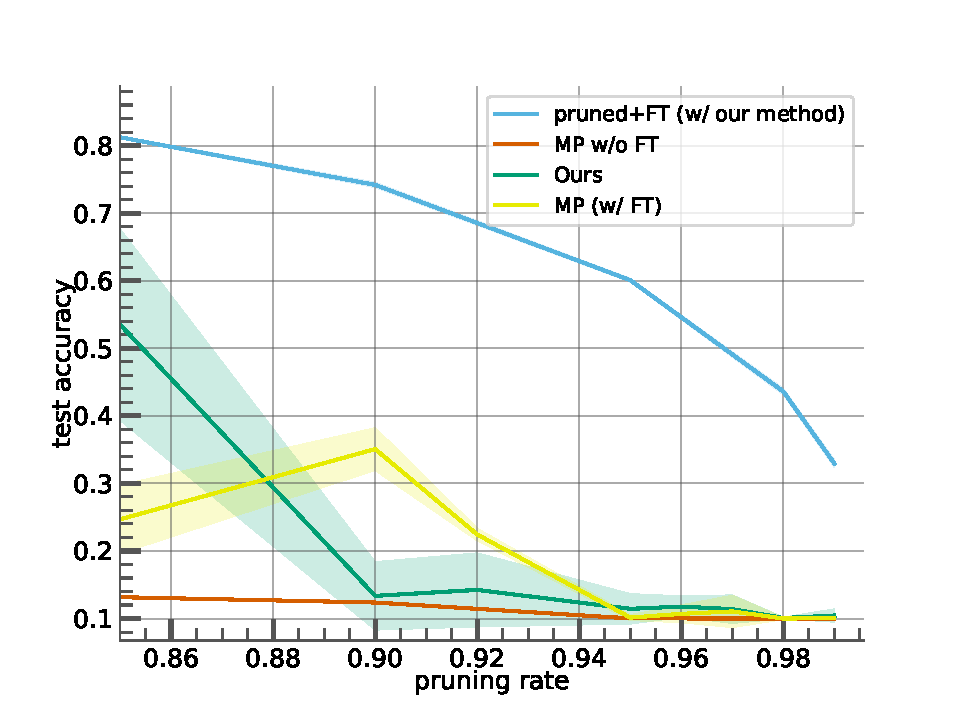
\includegraphics[width=0.49\textwidth]{chapter_1/assets/finetuning_cifar10_PrunableResNet20.pdf}}
    \subfloat[ResNet20
    CIFAR-100\label{fig:chap1:finetuning_impact_resnet20_cifar100}]{
    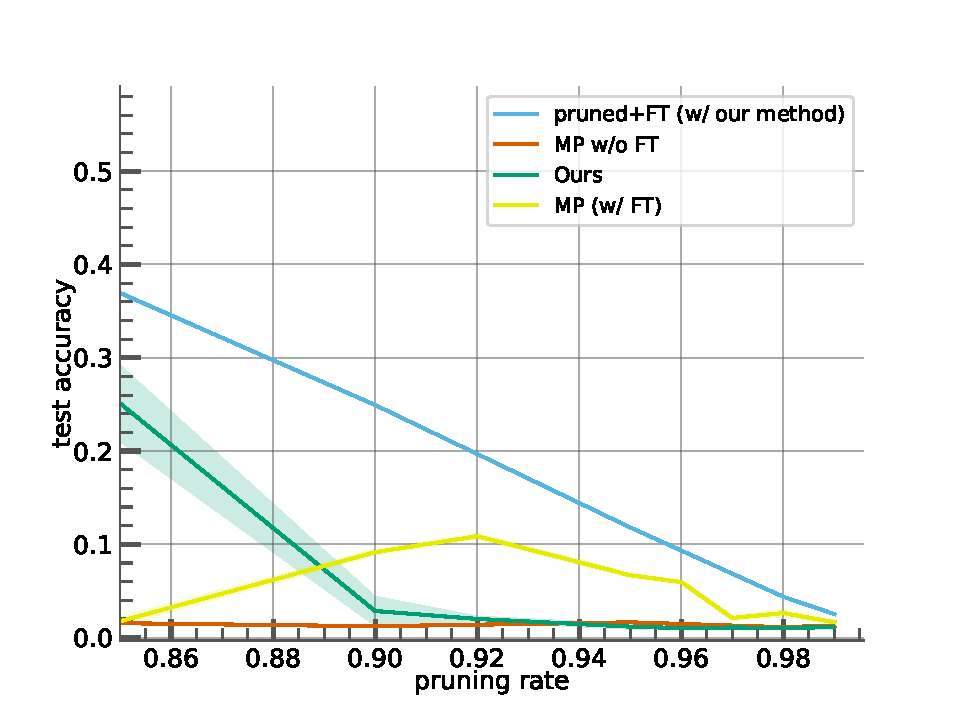
\includegraphics[width=0.49\textwidth]{chapter_1/assets/finetuning_cifar100_PrunableResNet20.pdf}}
    \caption{ Fine-tuning of a ResNet20 network pruned by magnitude pruning
    (\emph{MP w/o FT}) on the CIFAR-10 and CIFAR-100 datasets with various
    pruning rates. Conventional (\emph{MP w/ FT}) fine-tuning is compared to
    fine-tuning with our method (\emph{pruned+FT (w/ our method)}). Our method,
    described in \cref{sec:chap1:overview}, is shown for comparison purposes
    (\emph{Ours}). On this network, fine-tuning with our method considerably
    outperforms other approaches.}
  \label{fig:chap1:finetuning_impact_resnet20}
\end{figure}


\begin{figure}
  \centering
  \subfloat[VGG16 CIFAR-10\label{fig:chap1:finetuning_impact_vgg16_cifar10}]{
    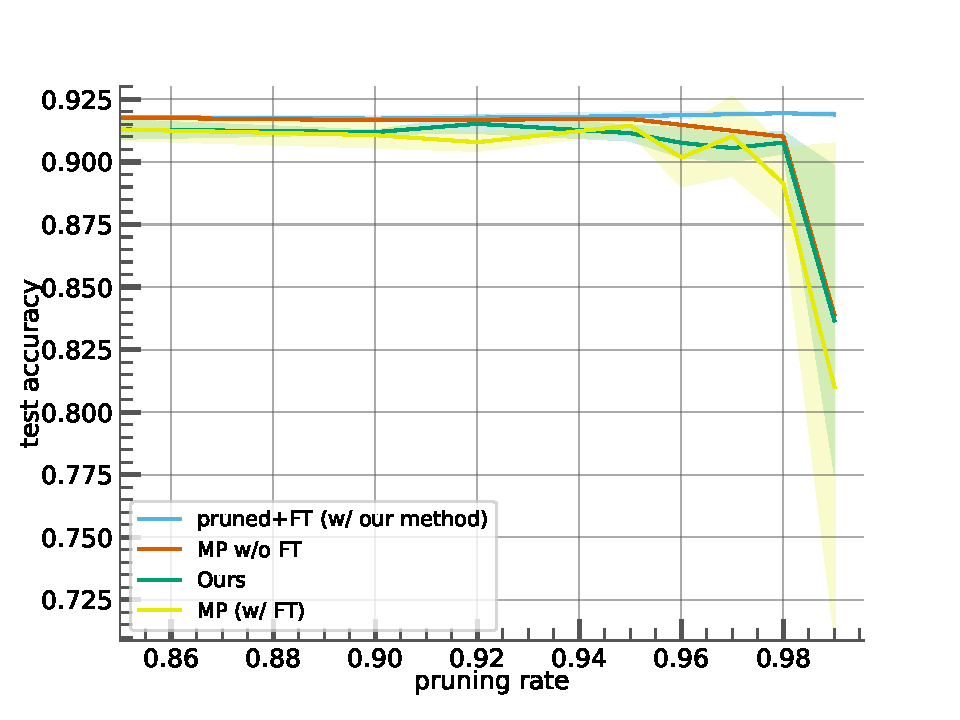
\includegraphics[width=0.49\textwidth]{chapter_1/assets/finetuning_cifar10_PrunableVGG16.pdf}}
  \subfloat[VGG16 CIFAR-100\label{fig:chap1:finetuning_impact_vgg16_cifar100}]{
    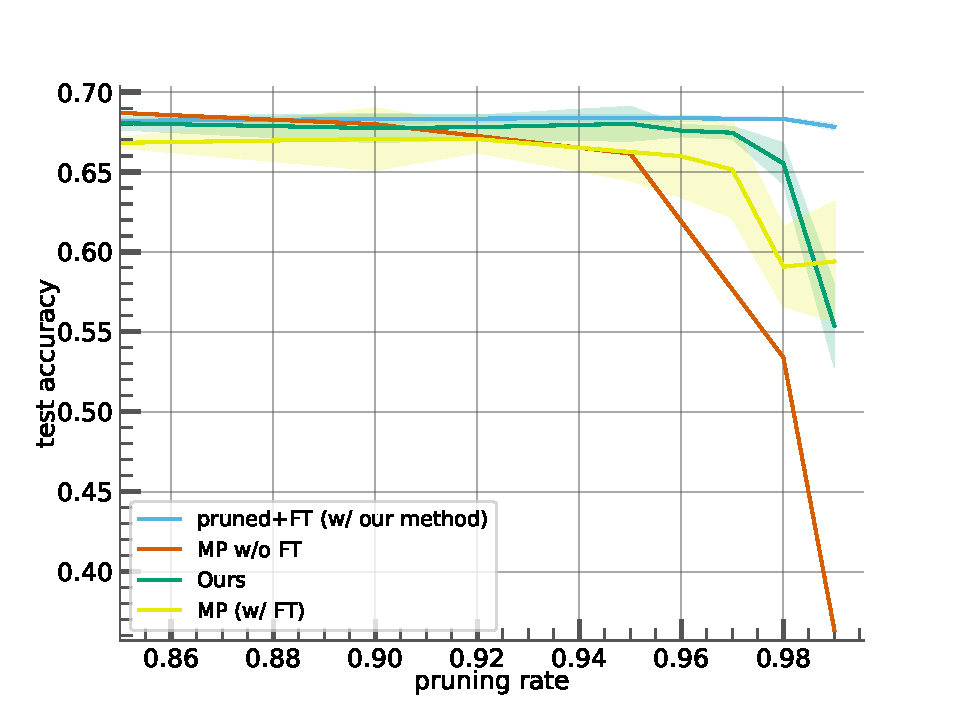
\includegraphics[width=0.49\textwidth]{chapter_1/assets/finetuning_cifar100_PrunableVGG16.pdf}}
  \caption{ Fine-tuning of a ResNet20 network pruned by magnitude pruning
    (\emph{MP w/o FT}) on the CIFAR-10 and CIFAR-100 datasets with various pruning
    rates. Conventional (\emph{MP w/ FT}) fine-tuning is compared to fine-tuning
    with our method (\emph{pruned+FT (w/ our method)}). Our method, described in
    \cref{sec:chap1:overview}, is shown for comparison purposes (\emph{Ours}). On
    this network, fine-tuning with our method performs on par with other methods
    up to 95\% of pruning. For higher pruning rates, it outperforms other
    approaches.}
  \label{fig:chap1:finetuning_impact_vgg6}
\end{figure}


\begin{figure}
  \centering
  \subfloat[Conv4 - CIFAR-10\label{fig:chap1:init_no_pruning_C4_C10}]{
    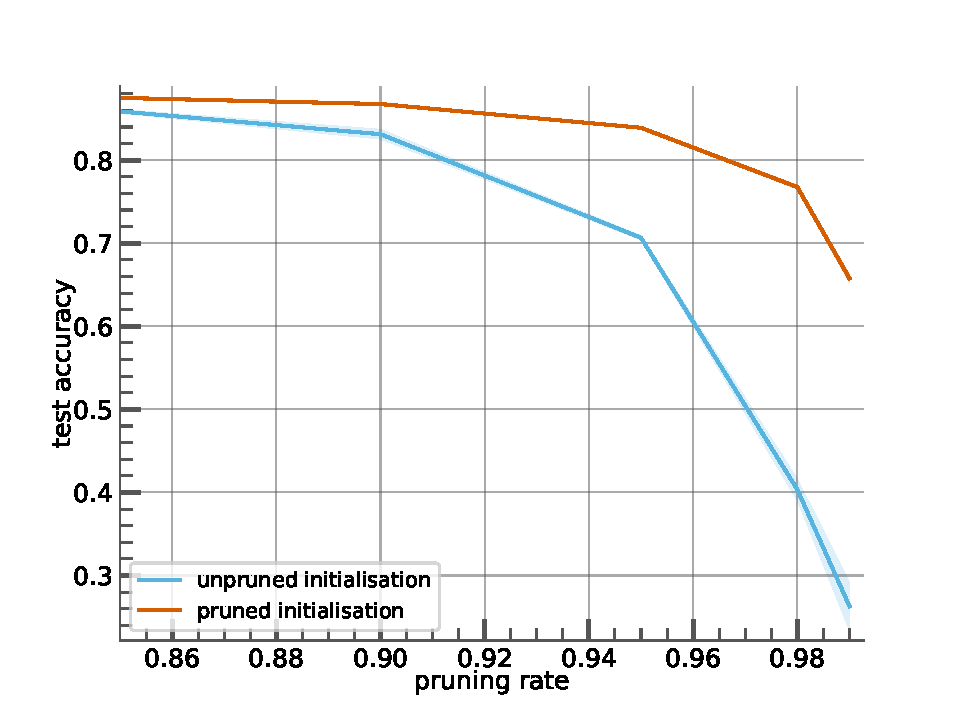
\includegraphics[width=0.4\textwidth]{chapter_1/assets/finetuning_init_not_pruned_cifar10_Conv4.pdf}}
  \subfloat[Conv4 - CIFAR-100\label{fig:chap1:init_no_pruning_C4_C100}]{
    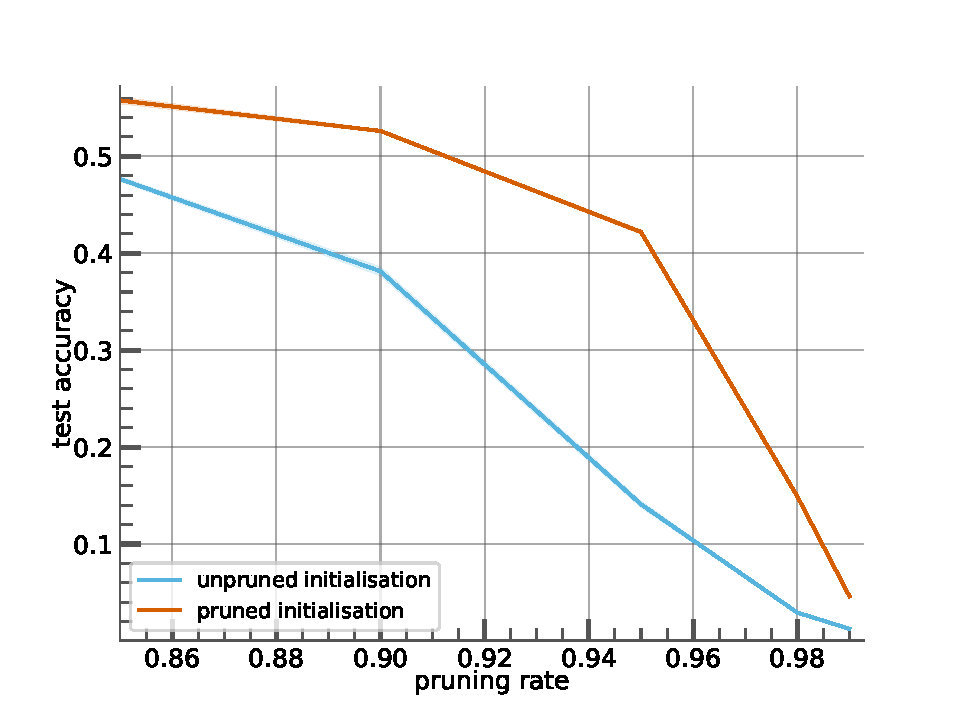
\includegraphics[width=0.4\textwidth]{chapter_1/assets/finetuning_init_not_pruned_cifar100_Conv4.pdf}}\\

  \subfloat[ResNet20 - CIFAR-10\label{fig:chap1:init_no_pruning_R20_C10}]{
    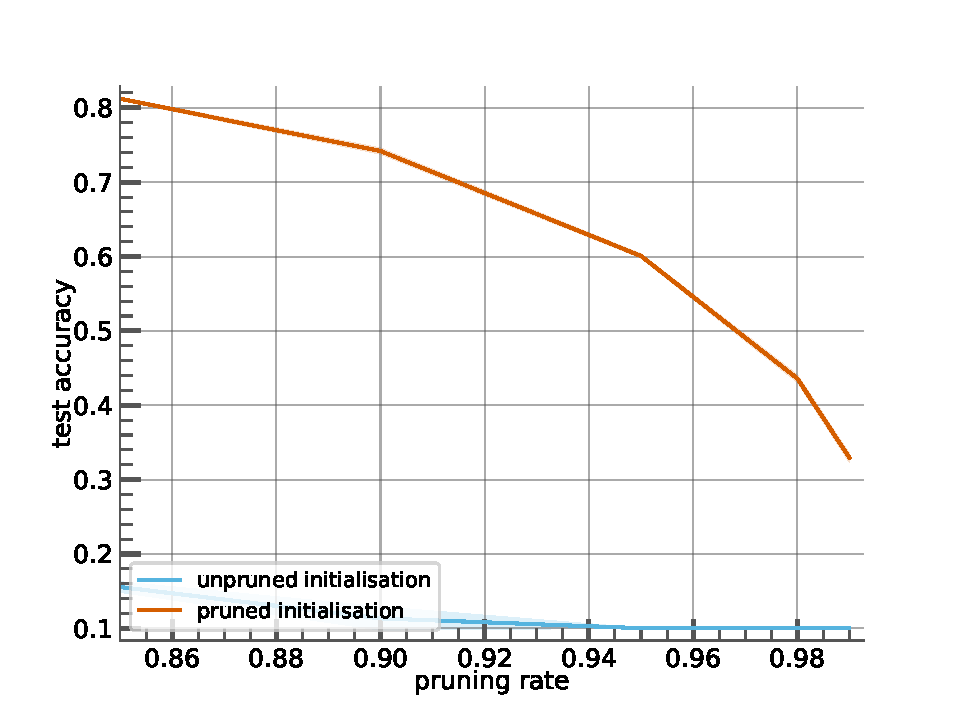
\includegraphics[width=0.4\textwidth]{chapter_1/assets/finetuning_init_not_pruned_cifar10_PrunableResNet20.pdf}}
  \subfloat[ResNet20 - CIFAR-100\label{fig:chap1:init_no_pruning_R20_C100}]{
    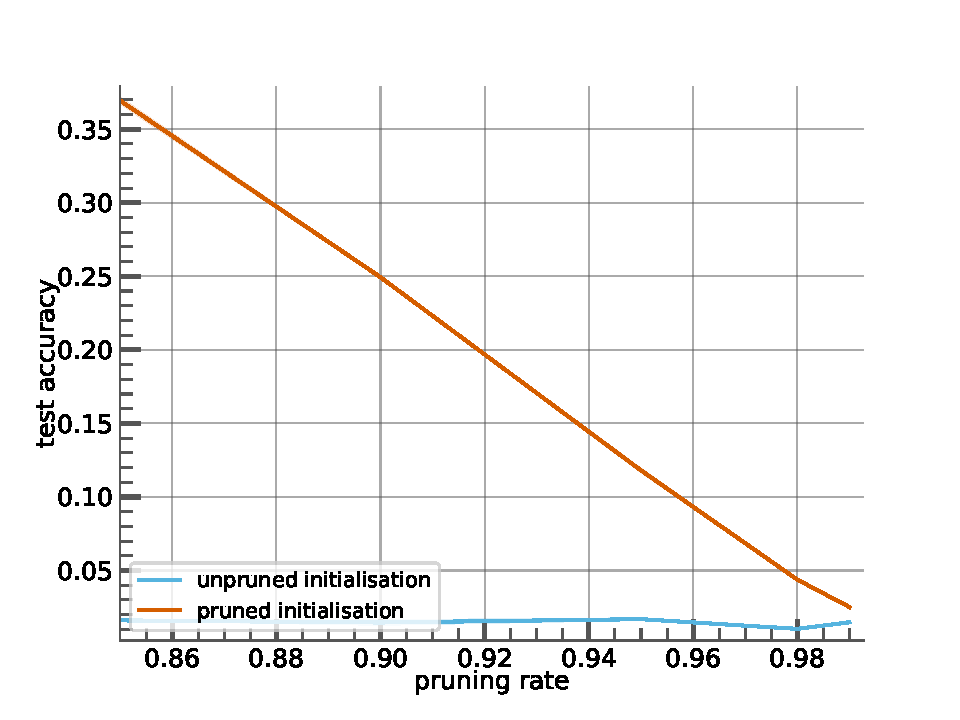
\includegraphics[width=0.4\textwidth]{chapter_1/assets/finetuning_init_not_pruned_cifar100_PrunableResNet20.pdf}}\\

  \subfloat[VGG16 - CIFAR-10\label{fig:chap1:init_no_pruning_VGG16_C10}]{
    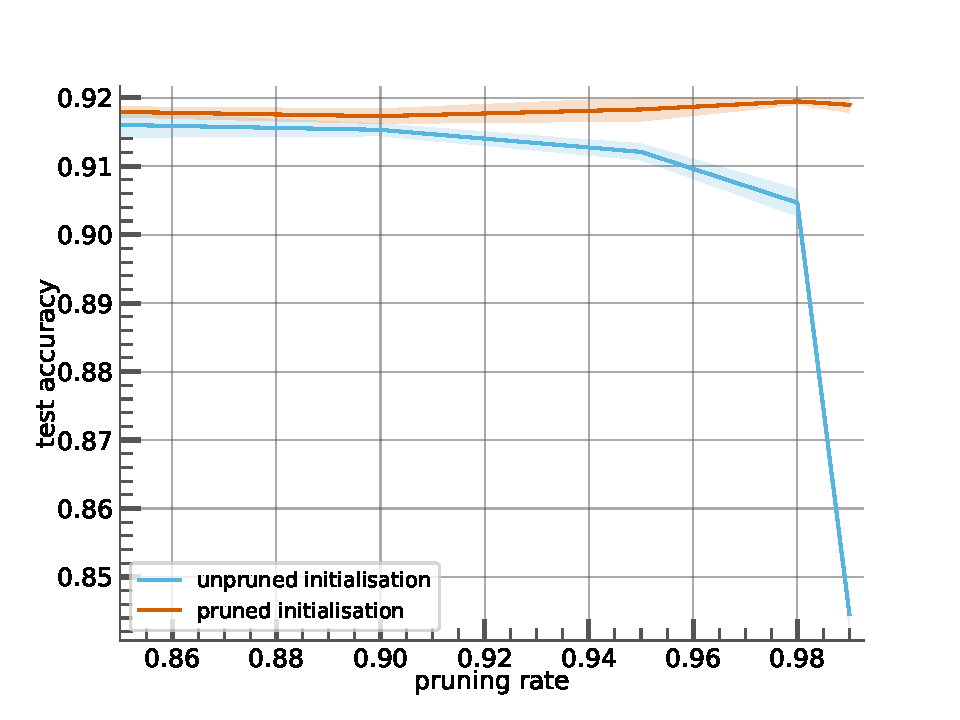
\includegraphics[width=0.4\textwidth]{chapter_1/assets/finetuning_init_not_pruned_cifar10_PrunableVGG16.pdf}}
  \subfloat[VGG16 - CIFAR-100\label{fig:chap1:init_no_pruning_VGG16_C100}]{
    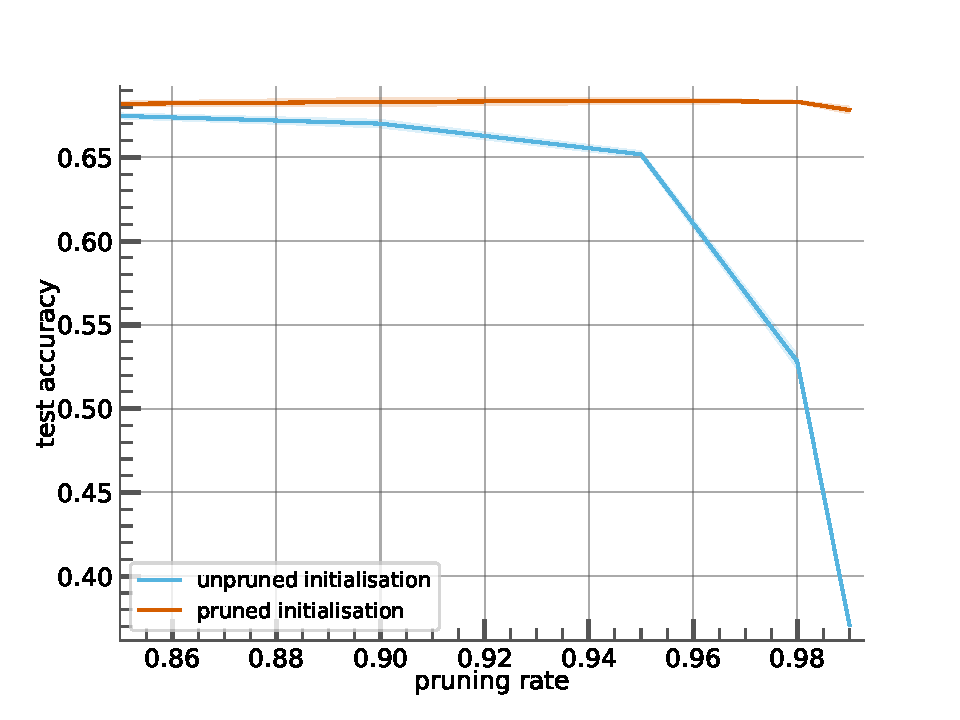
\includegraphics[width=0.4\textwidth]{chapter_1/assets/finetuning_init_not_pruned_cifar100_PrunableVGG16.pdf}}
  \caption{ Comparison of fine-tuning a network whose initialisation has been
    trained from scratch (denoted \emph{unpruned initialisation}) or trained from
    scratch and pruned with magnitude pruning (denoted \emph{pruned
      initialisation}). Fine-tuning a pruned initialisation always outperforms
    fine-tuning an unpruned initalisation in the tested configurations.}
  \label{fig:chap1:finetuning_with_init_not_pruned}

\end{figure}

% endregion: fine-tuning figs

% endregion: finetuning


\section{Conclusion}
\label{sec:chap1:conclusion}

% region: conclusion

This chapter introduces a novel approach for pruning neural networks, which
addresses the limitations of conventional pruning pipelines. The latter usually
apply a pruning criterion and prune networks after an initial training phase
without taking into account the target pruning rate. This often requires a
fine-tuning phase to restore the accuracy loss that follows pruning and the
subsequent topology alteration. In contrast, the proposed method does not
require fine-tuning to achieve superior performance compared to state-of-the-art
magnitude pruning methods. Experimental evaluations conducted on various
datasets and networks commonly used for image classification benchmarking
validate this claim.\\

Our approach described in this chapter consists of two key components: a budget
loss and a weight reparametrisation function. Comparative analyses demonstrate
the importance of both components, as variants without either the budget loss or
the reparametrisation, result in inferior performance compared to the
full-fledged method. While the proposed method is designed to avoid
computationally intensive fine-tuning, it can still be used for fine-tuning and
performs comparatively better than standard fine-tuning.\\

The proposed method of this chapter focuses on weight reparametrisation with
budget loss to enhance the network robustness to pruning: compared to a network
trained in the absence of such strategies, our use of reparametrisation and
budget loss substantially mitigates the performance degradation typically
induced by pruning. This forces less useful weights to take small values,
binding the weight value to the network topology. As such, the optimisation
process learns both the weights and topology under the hypothesis that weights
with smaller magnitudes will be removed. This method highlights the importance
of determining the optimal topology in addition to the optimal weights, achieved
in this chapter with the prior that magnitude is a saliency factor for weight
relevance in the topology.\\

Notwithstanding the improved performance of the proposed method compared to
magnitude pruning, it still suffers from some limitations. Namely, the value of
the weight saliency is bound to the reparametrisation which is in turn bound to
the weight value. As a consequence, the weight saliency is only determined by
the latter. The resulting limitation is that the current method cannot treat
weights with the same value (or similar values) differently. Put simply, the
topology is bound to the magnitude of the weights, but not their position in the
network.\\

In the next chapter, the introduced approach seeks to determine the optimal
topology without training the weights and without binding their saliency (or
relevance) to their magnitude. The saliency of the initial weights is determined
by a trained mask. In other words, the next method aims at determining the best
topology, given a set of fixed weights.\\

% endregion: conclusion